%Pre-amble to import suitable modules for a report
%\documentclass[draft]{article}
\documentclass[12pt]{article}
\usepackage[utf8]{inputenc}
%\usepackage[]{geometry}
\usepackage[a4paper, left=15mm, right=15mm, top=20mm, bottom=20mm]{geometry}
\usepackage[]{csvsimple}
\usepackage{graphicx}
\usepackage{enumitem}% http://ctan.org/pkg/enumitem
\setlist[itemize]{itemsep=-0.5ex,after=\vspace{\baselineskip}, topsep=-0.5ex} % requires enumitem package 
\setlist[enumerate]{itemsep=-0.5ex,after=\vspace{\baselineskip}, topsep=-0.5ex} % requires enumitem package 
\usepackage{xcolor} % allows defining your own colours
\usepackage[]{float}
\usepackage[]{caption}
\usepackage[titletoc]{appendix}
\usepackage{chngcntr}
\usepackage{tocbibind}
\usepackage{tabularx}
\usepackage{longtable}
\usepackage[]{multirow}
\usepackage{array} % to allow vertical alignment in tables
\usepackage{booktabs}
\usepackage{pgfplots}
\usepackage{pgfplotstable,filecontents} % enable import of csv files
\pgfplotsset{compat=1.8} % supress a warning or something
\usepackage{wrapfig} % allows figures to have text flow around it
\usepackage{subcaption}
\usepackage{amsmath} % le math
\usepackage{amsmath,amssymb,amsfonts,mathrsfs}
\allowdisplaybreaks
%\usepackage{lscape}
\usepackage{pdflscape} % enables insertion of pdf in landscape
\usepackage{color, colortbl}
	\definecolor{myPink}{cmyk}{0, 0.62, 0.47, 0}
    \definecolor{myRed1}{cmyk}{0, 0.89, 0.54, 0}    \definecolor{myRed2}{cmyk}{0, 0.89, 0.89, 0}
%\usepackage{hyperref} % uncomment after document is finished to hyperlink everything
%\hypersetup{
%    colorlinks,
%    linkcolor={red!50!black},
%    citecolor={green!30!black},
%    urlcolor={blue!80!black}
%}
\usepackage[export]{adjustbox} % enables setting figure height/width dimensions

%Change these dependent on report - including the main details - this will change the details in titlepage2.tex
\newcommand{\reporttitle}{Coursework}
\newcommand{\reportsupervisor}{Prof. Danilo P. Mandic}
\newcommand{\reporttype}{EE4-13 Adaptive Signal Processing and Machine Intelligence (2018-2019)}
\newcommand{\wordcount}{0}
\date{April 2019}

\renewcommand\thesection{\arabic{section}} % Define alphabetical numeration vs. arabic numbering
\renewcommand\thesubsection{\thesection.\arabic{subsection}}
\renewcommand\thesubsubsection{\thesubsection.\alph{subsubsection}}

% Expectation & Variance symbol
\DeclareMathOperator*{\E}{\mathbb{E}}
\DeclareMathOperator*{\Var}{\mathbb{V}}
% Correlation
\DeclareMathOperator{\Corr}{Corr}

\begin{document}
% Last modification: 2018-03-30 (Adel Haddad)
\begin{titlepage}

\newcommand{\HRule}{\rule{\linewidth}{0.5mm}} % Defines a new command for the horizontal lines, change thickness here


%----------------------------------------------------------------------------------------
%	LOGO SECTION
%----------------------------------------------------------------------------------------


\includegraphics[width = 4cm, keepaspectratio]{imperial.pdf}\\
\vspace{0.25cm}

\begin{center} % Center remainder of the page

%----------------------------------------------------------------------------------------
%	HEADING SECTIONS
%----------------------------------------------------------------------------------------
\textsc{\LARGE \reporttype}\\[0.5cm] 
\textsc{\Large Imperial College London}\\[0.25cm] 
\textsc{\large Department of Electrical and Electronic Engineering}\\[0.5cm] 
%----------------------------------------------------------------------------------------
%	TITLE SECTION
%----------------------------------------------------------------------------------------

\HRule \\[0.4cm]
{ \huge \bfseries \reporttitle}\\ % Title of your document
\HRule \\[1.5cm]
\end{center}
%----------------------------------------------------------------------------------------
%	AUTHOR SECTION
%----------------------------------------------------------------------------------------

%\begin{minipage}{0.4\hsize}

\begin{flushleft} \large

\begin{tabbing} 
\hspace{55mm} \= \hspace{10pt} \=\\
\textit{Authors:} \> \> {CID}\\
\hspace{2mm} Adel Haddad		\>  01060023 \\
\end{tabbing} 

% Your name
\vspace{5mm}

\textit{Supervisor:}\\
\hspace{2mm} \reportsupervisor
\end{flushleft}
\vspace{6mm}
\makeatletter
Date: \@date\\
Word Count: \wordcount

\vspace*{\fill} % Fill the rest of the page with whitespace, vertically centering whatever is inside
{
\begin{center}
	\vspace{1.5cm}
	
\includegraphics[width = 4.5cm]{ICL-crest.pdf}\\
\end{center}

}
\vspace*{\fill} 
\clearpage % make sure the text afterwards is not centered in anyway


\makeatother


\end{titlepage}



%\maketitle

\newpage
\tableofcontents

\newpage
\section{Classical and Modern Spectrum Estimation}
	\subsection{Properties of Power Spectral Density (PSD)} \label{sec: 1-1-prop-PSD}
	
	\subsubsection{Approximation in the Definition of PSD} \label{sec: 1-1a-prop-PSD}
	Starting with the equation provided, (\ref{proof: periodogram:starter}), we: use the relationship between modulus and complex conjugate for complex numbers, we move out the summation terms from the expectation operator, we factor out the exponential terms - as they are independent of the random variable $x$ and we finally use the property that the expectation of a complex conjugate is .........
	\begin{align}
		P(\omega)   & =\lim_{N\to\infty} \E \bigg\{ \frac{1}{N} \bigg| \sum_{n=0}^{N-1} x(n) e^{-j\omega n} \bigg|^{2} \bigg\}
		\label{proof: periodogram:starter}\\
		& = \lim_{N\to\infty} \E \bigg\{\frac{1}{N}
		\sum_{m=0}^{N-1} x(m) e^{-j\omega m} \sum_{k=0}^{N-1} x^{*}(k) e^{j\omega k} \bigg\}\nonumber\\
		& = \lim_{N\to\infty} \frac{1}{N}
		\sum_{m=0}^{N-1} \sum_{k=0}^{N-1} \E \bigg\{ x(m) e^{-j\omega m} x^{*}(k) e^{j\omega k} \bigg\}\nonumber\\
		& = \lim_{N\to\infty} \frac{1}{N}
		\sum_{m=0}^{N-1} \sum_{k=0}^{N-1} \E \bigg\{ x(m) x^{*}(k) \bigg\} e^{-j\omega(m-k)} \nonumber\\
		& = \lim_{N\to\infty} \frac{1}{N}
		\sum_{m=0}^{N-1} \sum_{k=0}^{N-1} r_{xx}(m-k) e^{-j\omega(m-k)}
		= \lim_{N\to\infty} \frac{1}{N}
		\sum_{m=0}^{N-1} \sum_{k=0}^{N-1} g(m-k)
		\label{proof: periodogram}
	\end{align}
	
	where $g(\tau) = r_{xx}(\tau) e^{-j\omega\tau}$
	\newline
	We can convert the double summation into a single summation using:
	
	\begin{equation}
		\sum_{m=-N}^{N} \sum_{k=-N}^{N} g(m-k) = \sum_{\tau=-2N}^{2N}(2N + 1 - |\tau|)g(\tau)
		\label{proof: periodogram:helper}
	\end{equation}
	\newline
	(\ref{proof: periodogram}) can then be written as:
	\vspace{-\baselineskip}
	\begin{align}
		P(\omega)    & =         \lim_{N\to\infty} \frac{1}{N} \sum_{\tau=-(N-1)}^{N-1}(N - |\tau|)r_{xx}(\tau) e^{-j\omega\tau}\nonumber\\
		& =         \lim_{N\to\infty} \sum_{\tau=-(N-1)}^{N-1} r_{xx}(\tau) e^{-j\omega\tau} -
		\lim_{N\to\infty} \frac{1}{N} |\tau| \sum_{\tau=-(N-1)}^{N-1} r_{xx}(\tau) e^{-j\omega\tau}\nonumber\\
		& \approx   \sum_{\tau=-\infty}^{\infty} r_{xx}(\tau) e^{-j\omega\tau}
		\label{proof: periodogram:shown}
	\end{align}
	
	\subsubsection{Simulation of the Limiting Case} \label{sec: 1-1b-prop-PSD}
	
	
	\subsection{Periodogram-based Methods Applied to Real–World Data} \label{sec: 1-2-PSD-real-world}
	\subsubsection{The SunSpot Dataset}
	I am putting some text

	\begin{figure}[H]
		\centering
		\begin{subfigure}{0.49\textwidth}
			\centering
			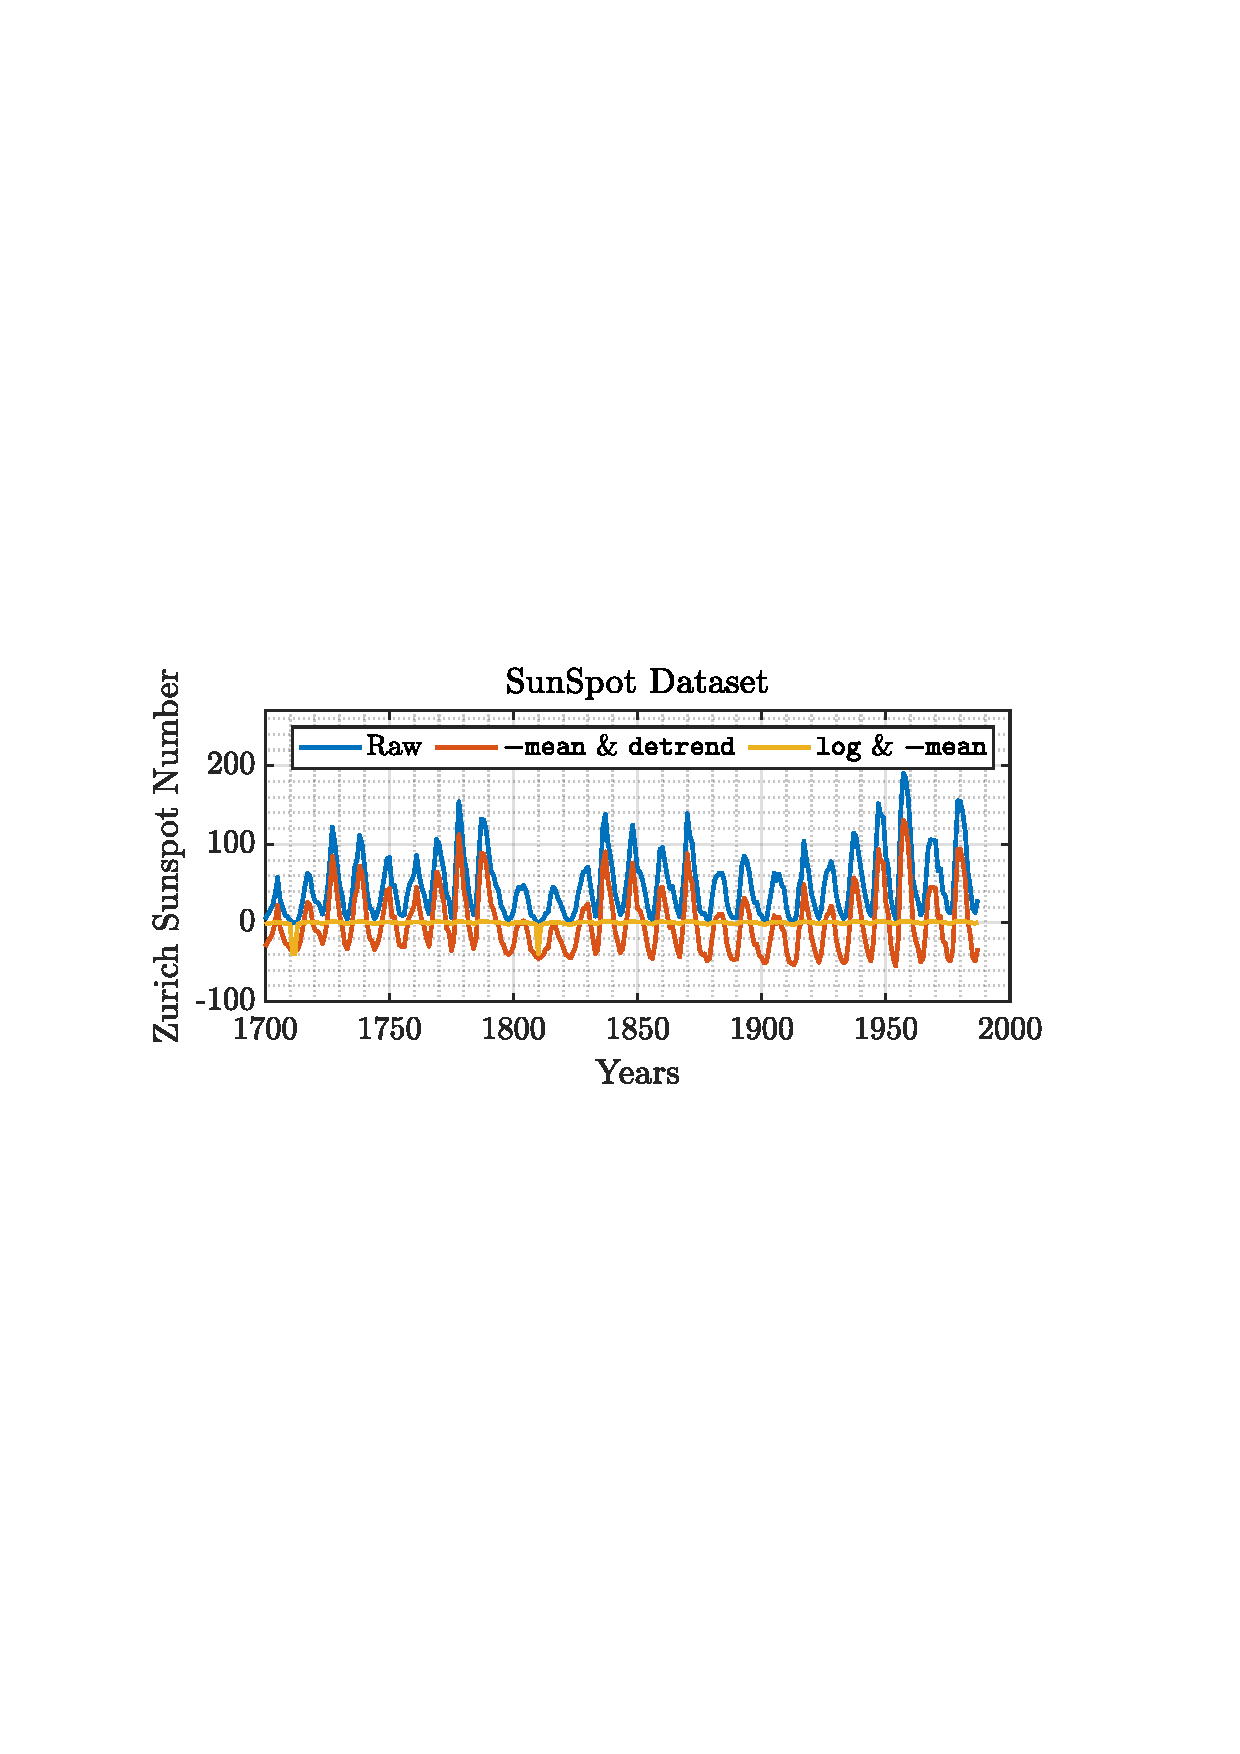
\includegraphics[trim={2.2cm 11.2cm 3.15cm  11.2cm}, clip, width=\textwidth]{../MATLAB/figures/q1_2a_fig01.pdf} 
			\captionsetup{justification=centering}
			\caption{Raw and its preprocessed datas}
		\end{subfigure}
%		~ % forces onto the same row
		\begin{subfigure}{0.49\textwidth}
			\centering
			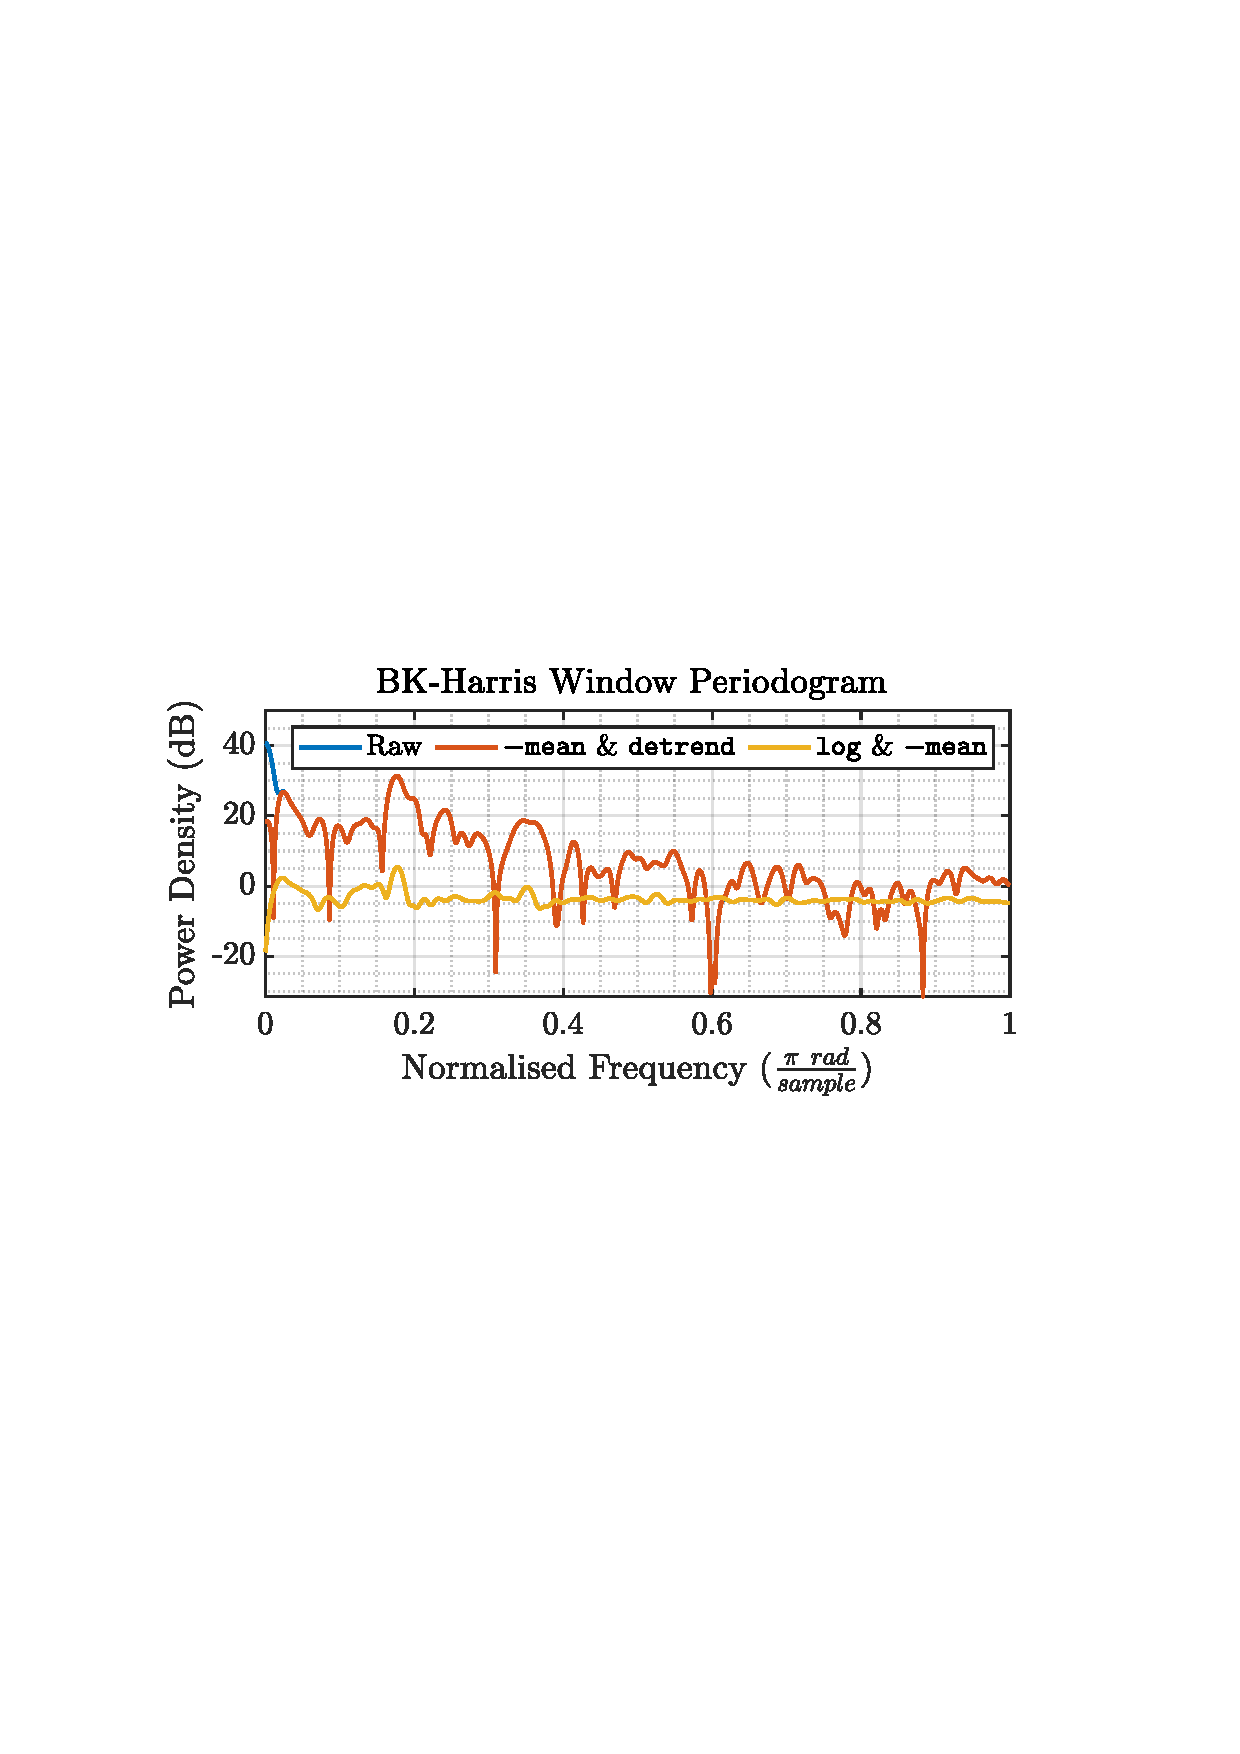
\includegraphics[trim={2.2cm 11.2cm 3.15cm  11.2cm}, clip, width=\textwidth]{../MATLAB/figures/q1_2a_fig02.pdf} 
			\captionsetup{justification=centering}
			\caption{Periodograms}
		\end{subfigure}
		\label{fig: 1-2a}
	\end{figure}
%	\begin{figure}[H]
%		\centering
%		%\begin{subfigure}[t]{0.4\textwidth}
%		%	\centering
%		%\hspace*{-2.1cm}
%		% 				trim={<left> <lower> <right> <upper>}
%		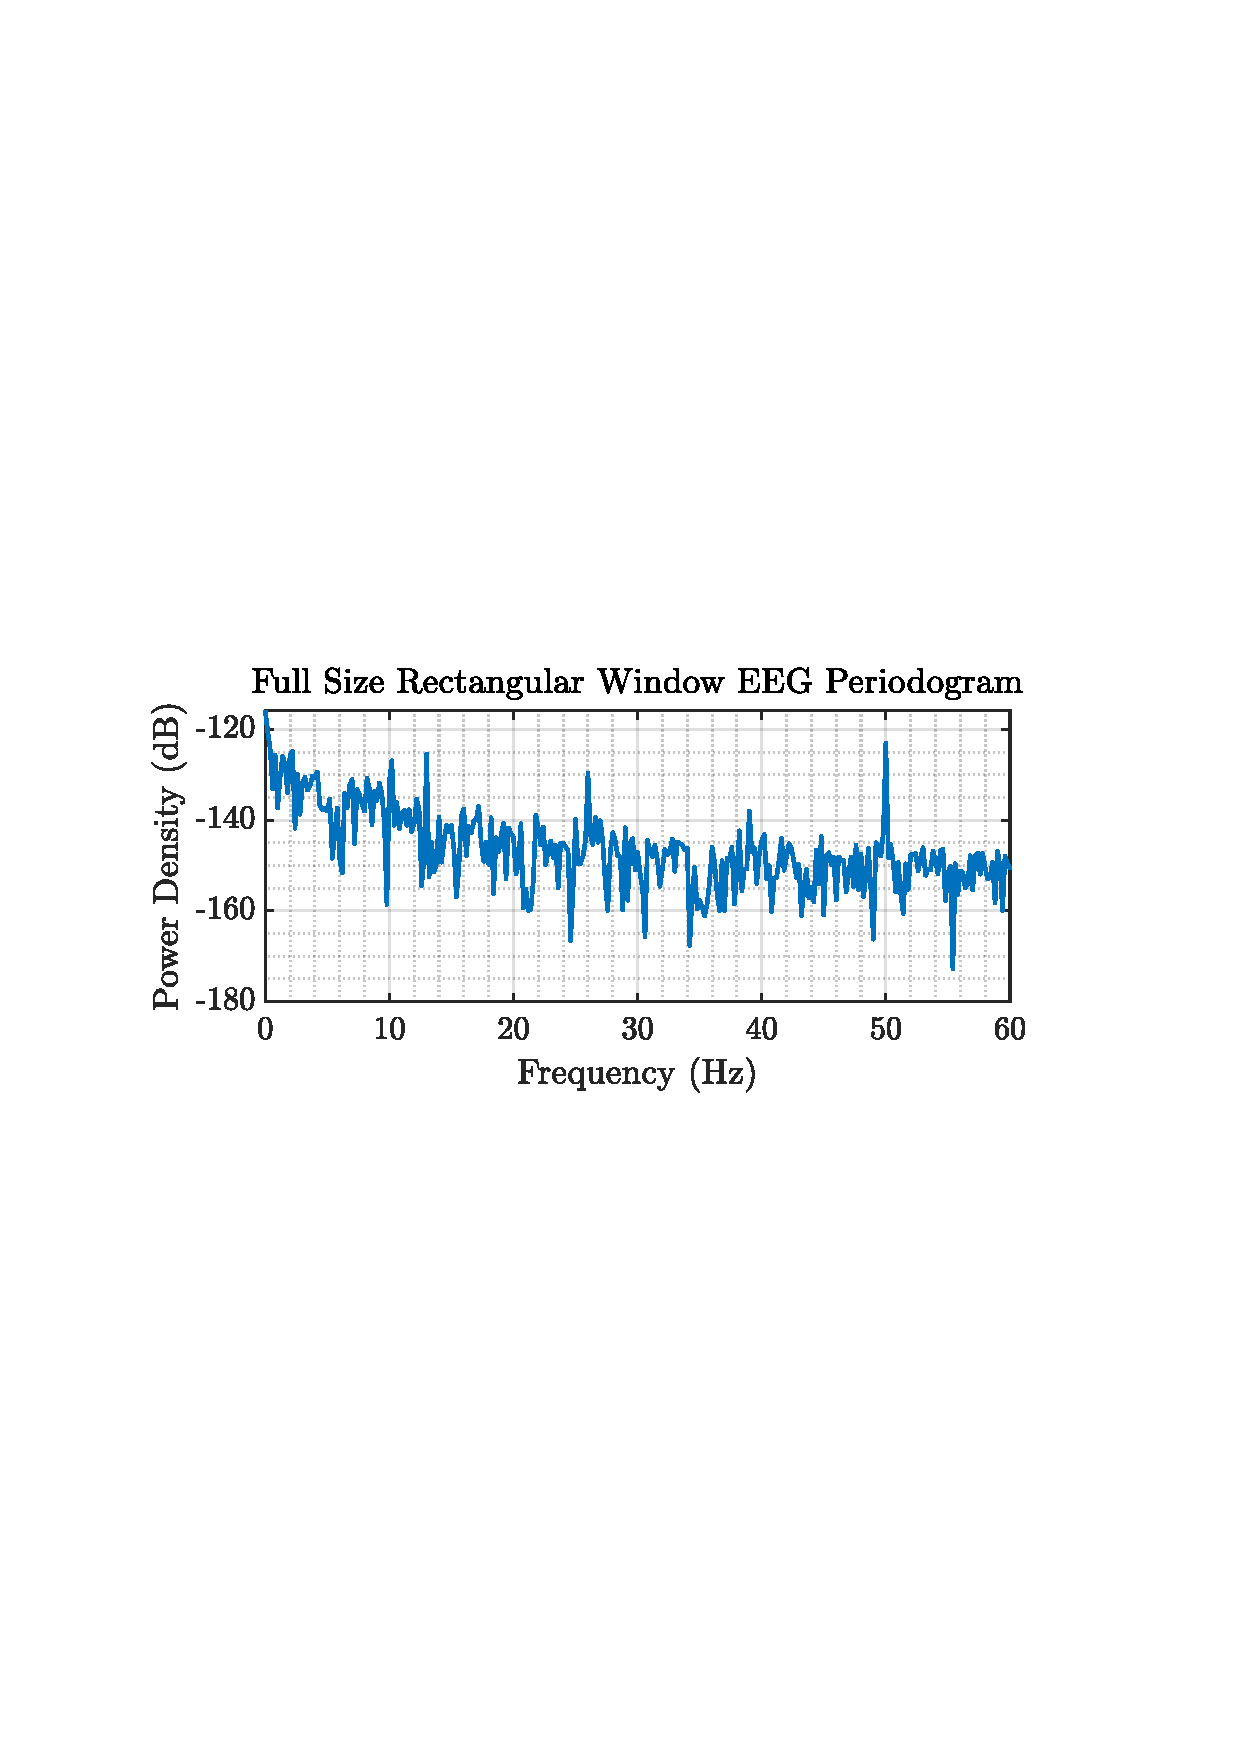
\includegraphics[trim={2.2cm 11.2cm 3.15cm  11.2cm}, clip, width=9cm]{../MATLAB/figures/q1_2b_fig01.pdf} 
%		%	\captionsetup{justification=centering}
%		%	\caption{Vertical gel electrophoresis setup} 
%		%	\label{fig: verticalGel}
%		%\end{subfigure}
%		%\hfill
%		\captionsetup{justification=centering}
%		\caption{Science being done here}
%	\end{figure}


	\subsubsection{The ECG Dataset}
	% TODO: the title's say EEG but it is an ECG
	\begin{figure}[H]
		\centering
		\begin{subfigure}{0.49\textwidth}
			\centering
			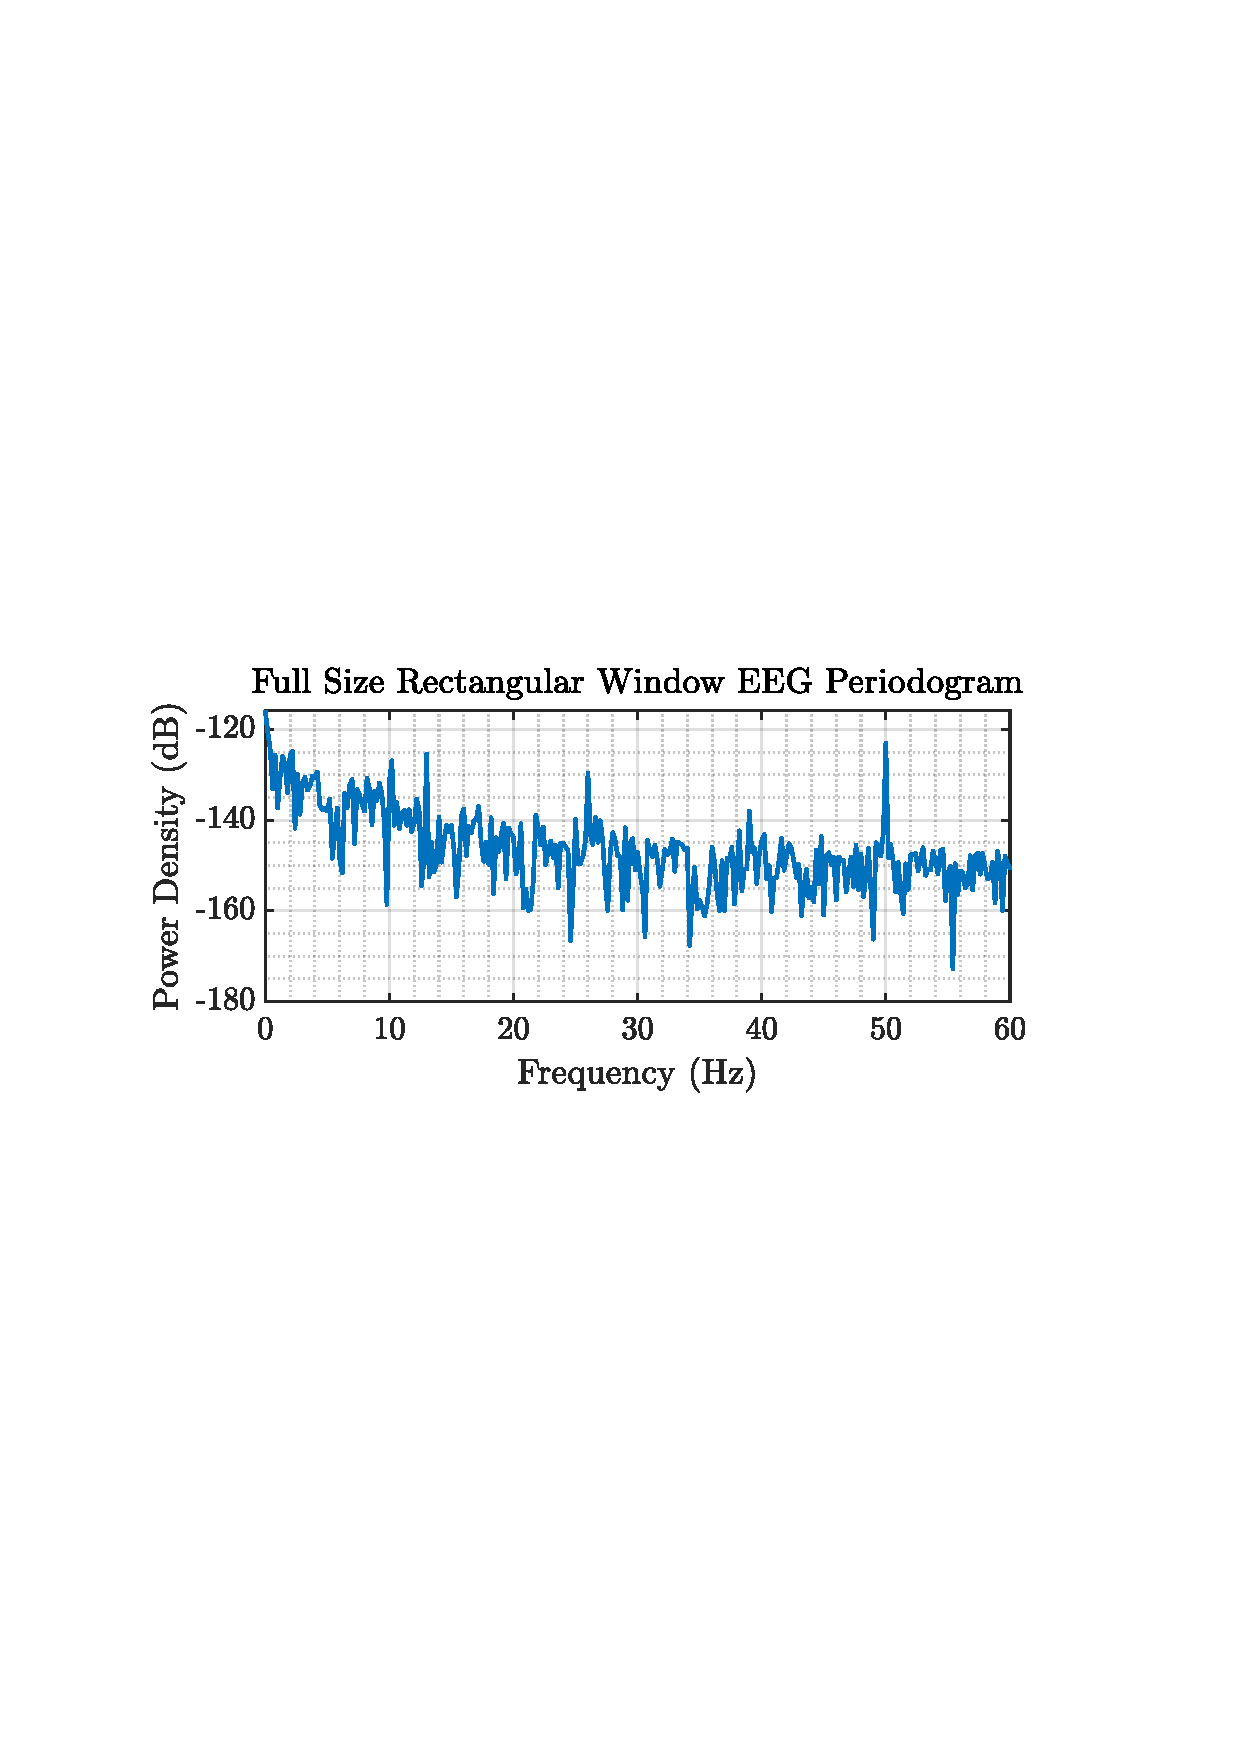
\includegraphics[trim={2.2cm 11.2cm 3.15cm  11.2cm}, clip, width=\textwidth]{../MATLAB/figures/q1_2b_fig01.pdf} 
			\captionsetup{justification=centering}
			\caption{Standard Periodogram}
		\end{subfigure}
		%		~ % forces onto the same row
		\begin{subfigure}{0.49\textwidth}
			\centering
			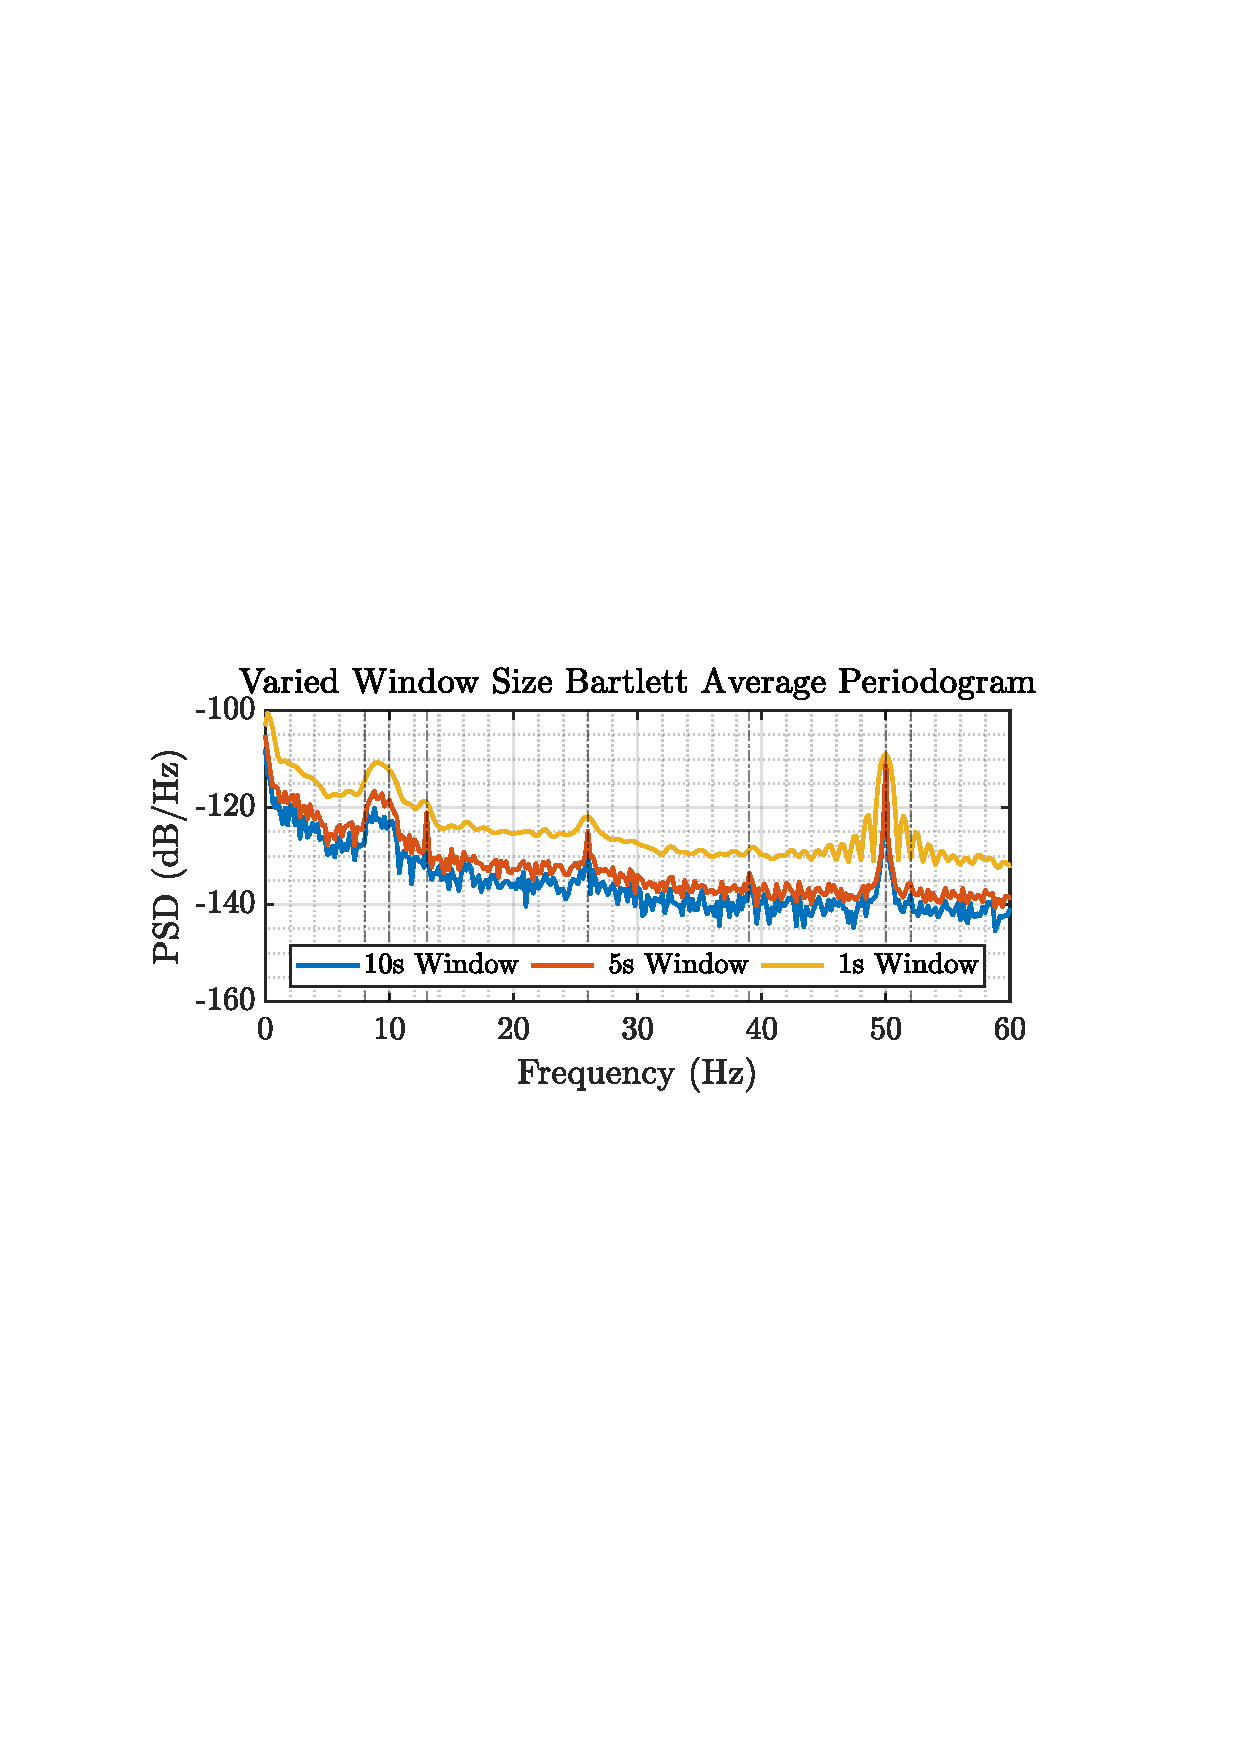
\includegraphics[trim={2.2cm 11.2cm 3.15cm  11.2cm}, clip, width=\textwidth]{../MATLAB/figures/q1_2b_fig02.pdf} 
			\captionsetup{justification=centering}
			\caption{Bartlett Average Periodograms}
		\end{subfigure}
		\label{fig: 1-2b}
	\end{figure}

	\subsection{Correlation Estimation} \label{sec: 1-3-correlation-est}
	
	\subsubsection{Unbiased and Biased ACF Estimates}
	
	\begin{figure}[H]
		\centering
		\begin{subfigure}{0.49\textwidth}
			\centering
			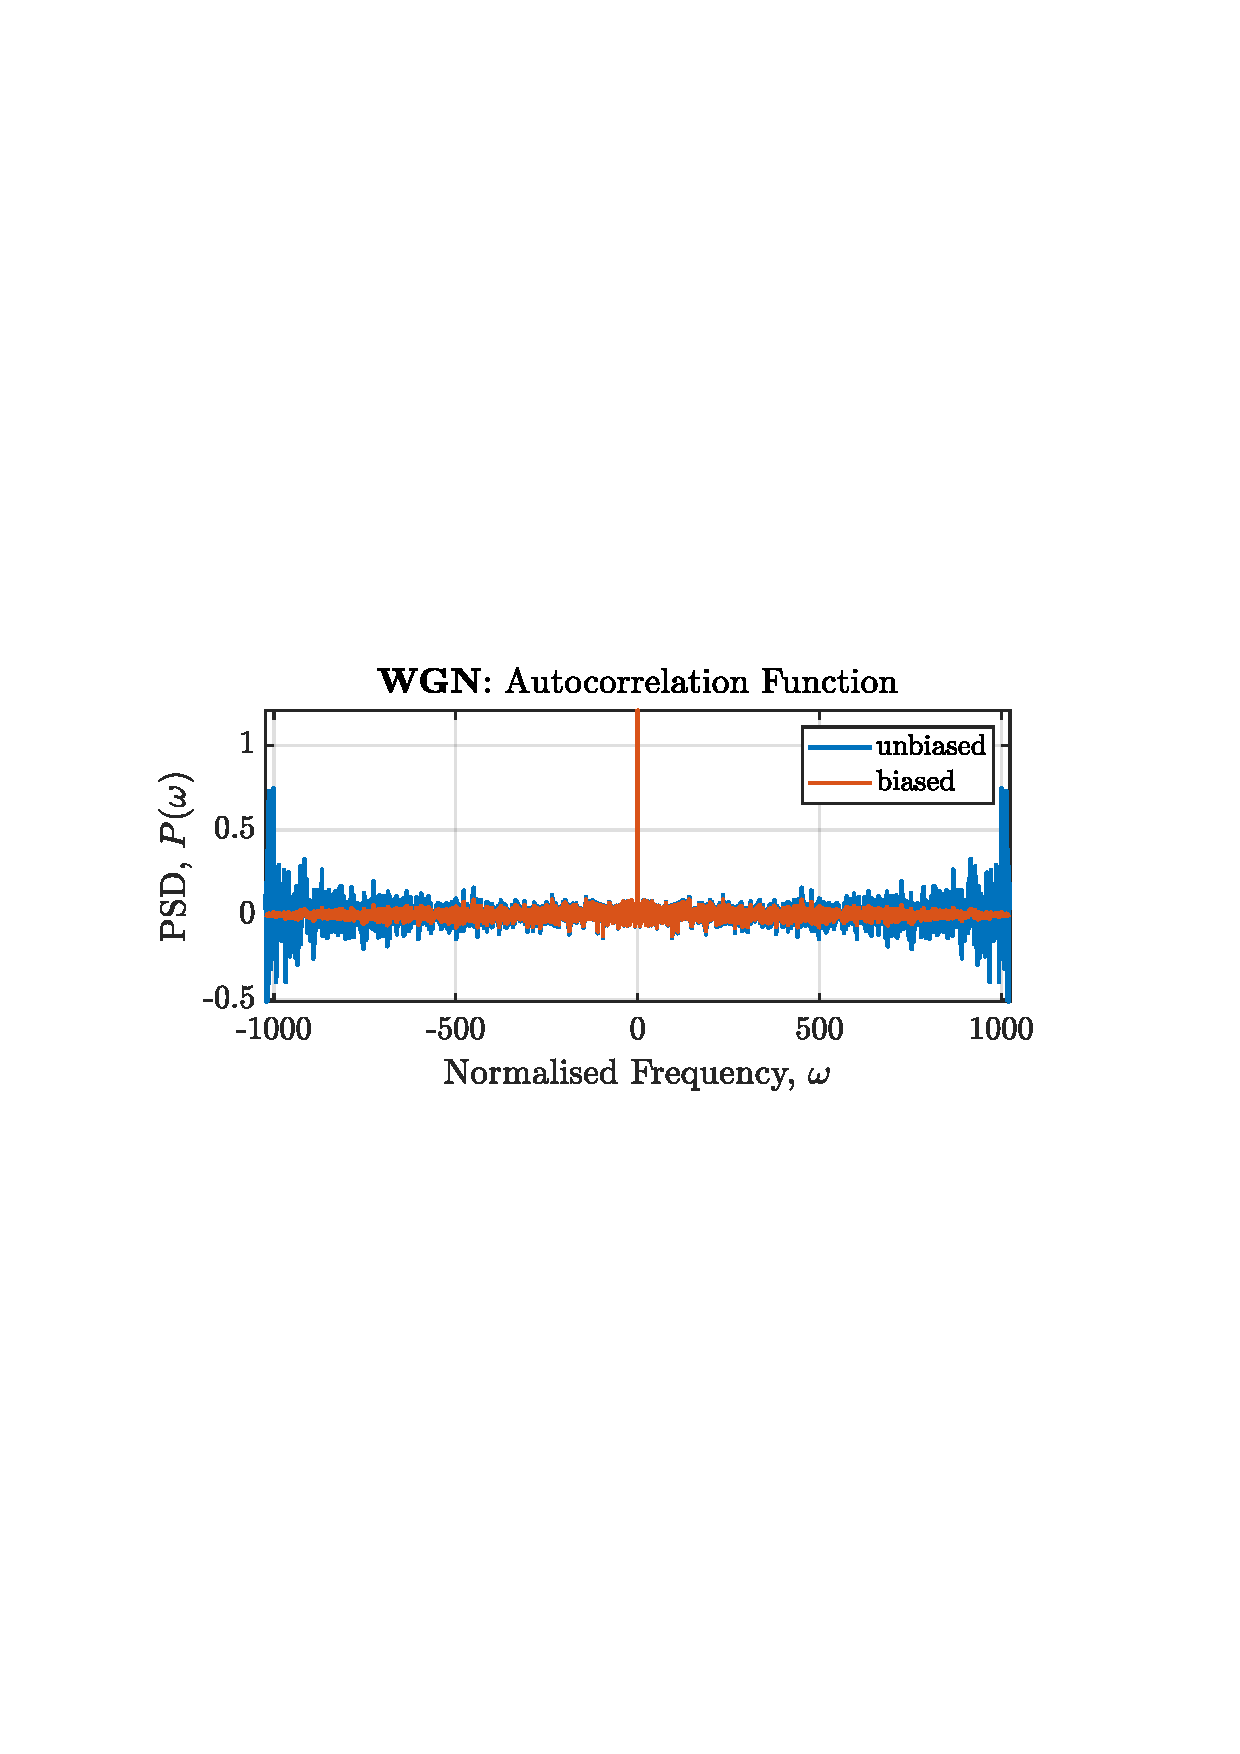
\includegraphics[trim={2.2cm 11cm 3.15cm  11.2cm}, clip, width=\textwidth]{../MATLAB/figures/q1_3a_fig01.pdf} 
		\end{subfigure}
		%		~ % forces onto the same row
		\begin{subfigure}{0.49\textwidth}
			\centering
			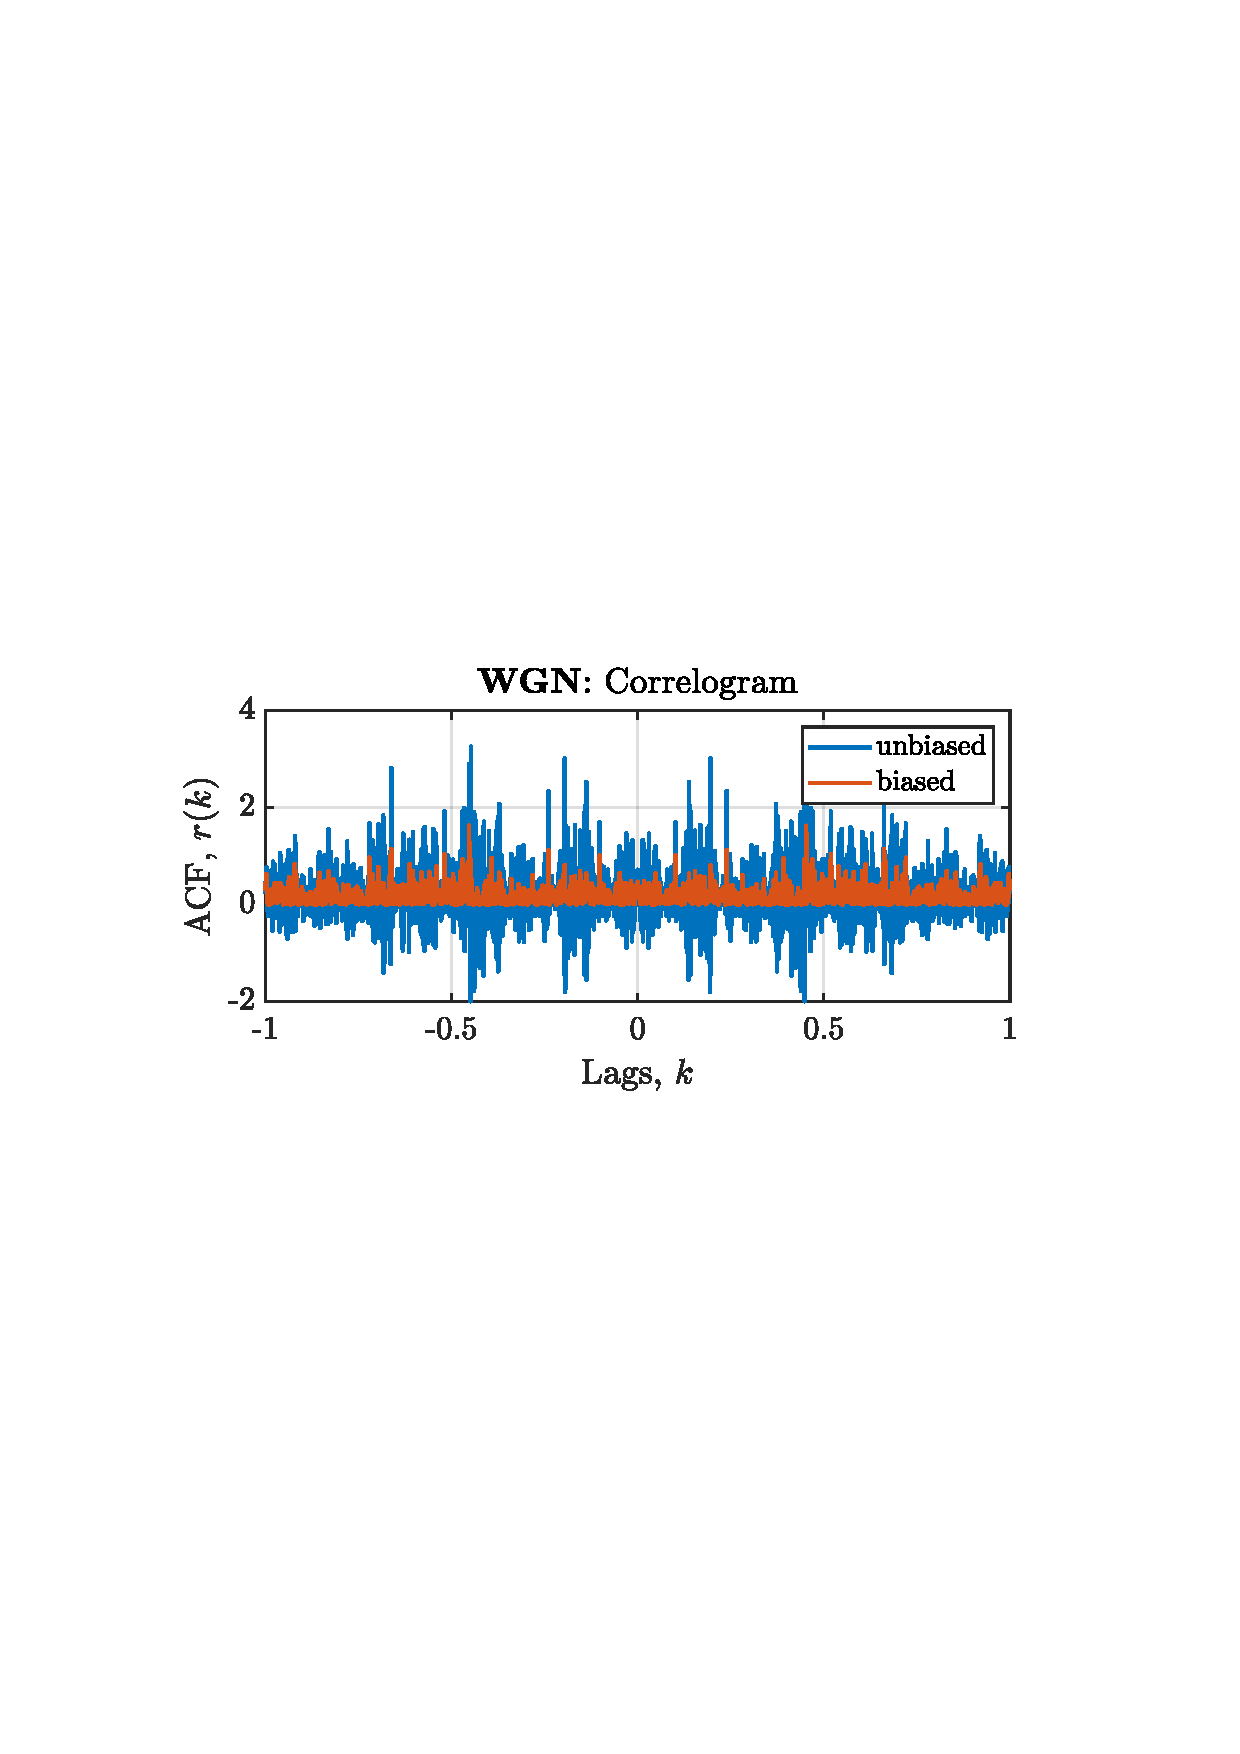
\includegraphics[trim={2.2cm 11cm 3.15cm  11.2cm}, clip, width=\textwidth]{../MATLAB/figures/q1_3a_fig02.pdf} 
		\end{subfigure}
				\begin{subfigure}{0.49\textwidth}
			\centering
			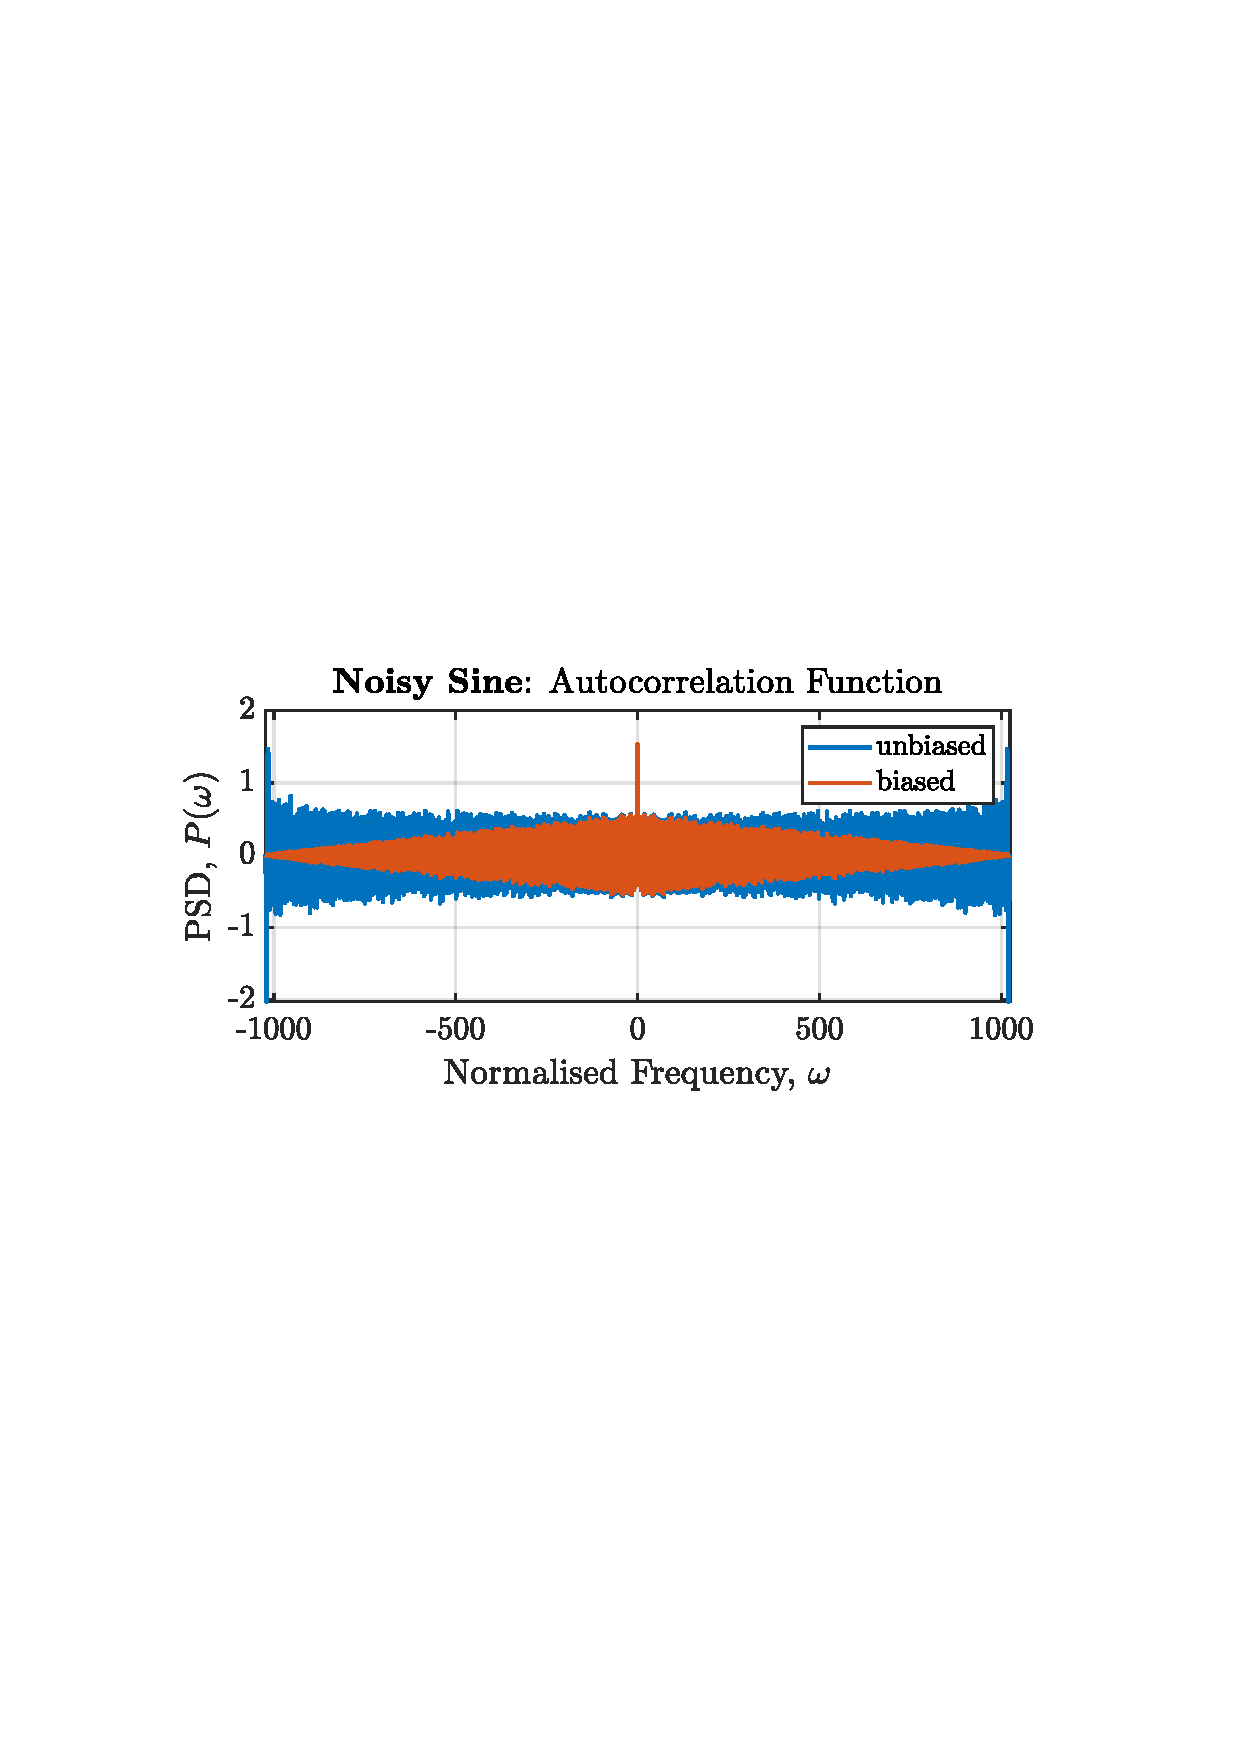
\includegraphics[trim={2.2cm 11cm 3.15cm  11.2cm}, clip, width=\textwidth]{../MATLAB/figures/q1_3a_fig03.pdf} 
		\end{subfigure}
		%		~ % forces onto the same row
		\begin{subfigure}{0.49\textwidth}
			\centering
			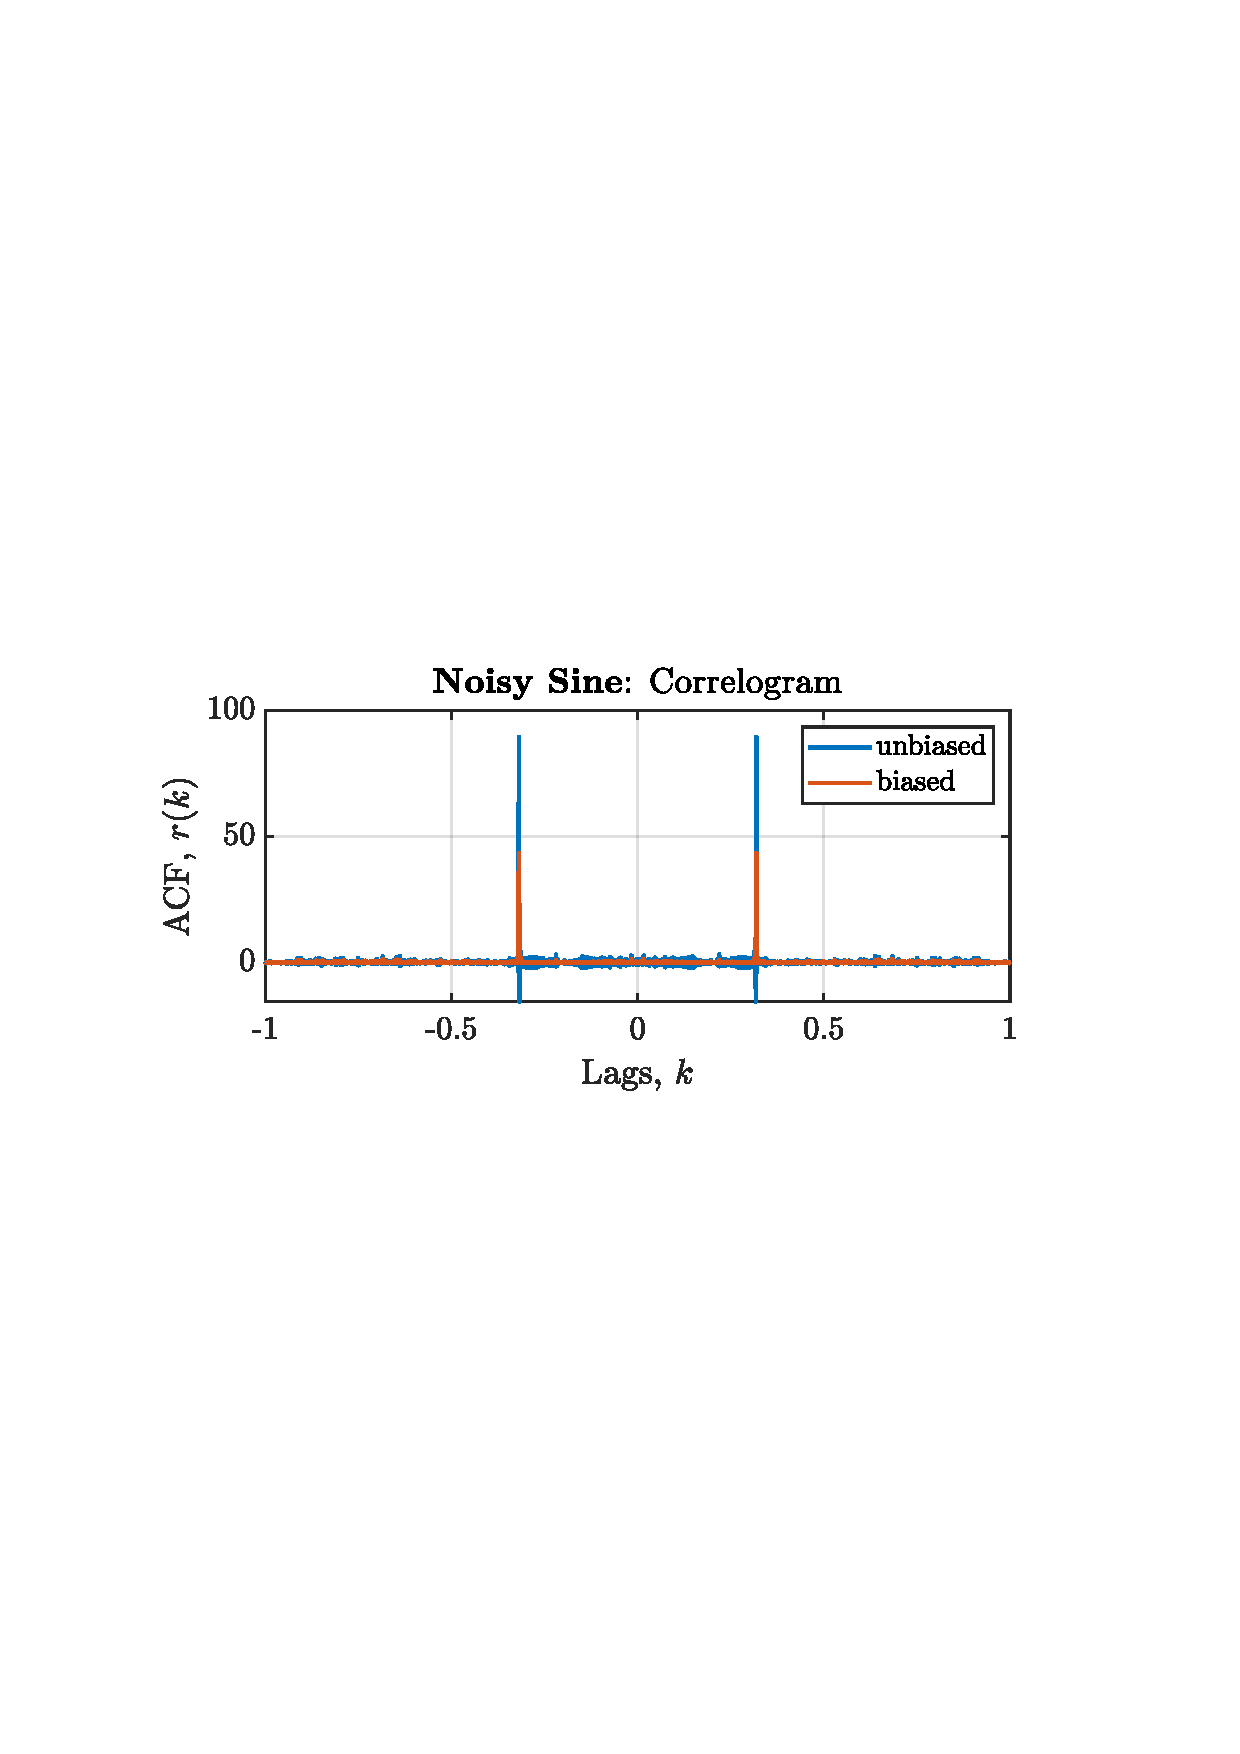
\includegraphics[trim={2.2cm 11cm 3.15cm  11.2cm}, clip, width=\textwidth]{../MATLAB/figures/q1_3a_fig04.pdf} 
		\end{subfigure}
		\begin{subfigure}{0.49\textwidth}
			\centering
			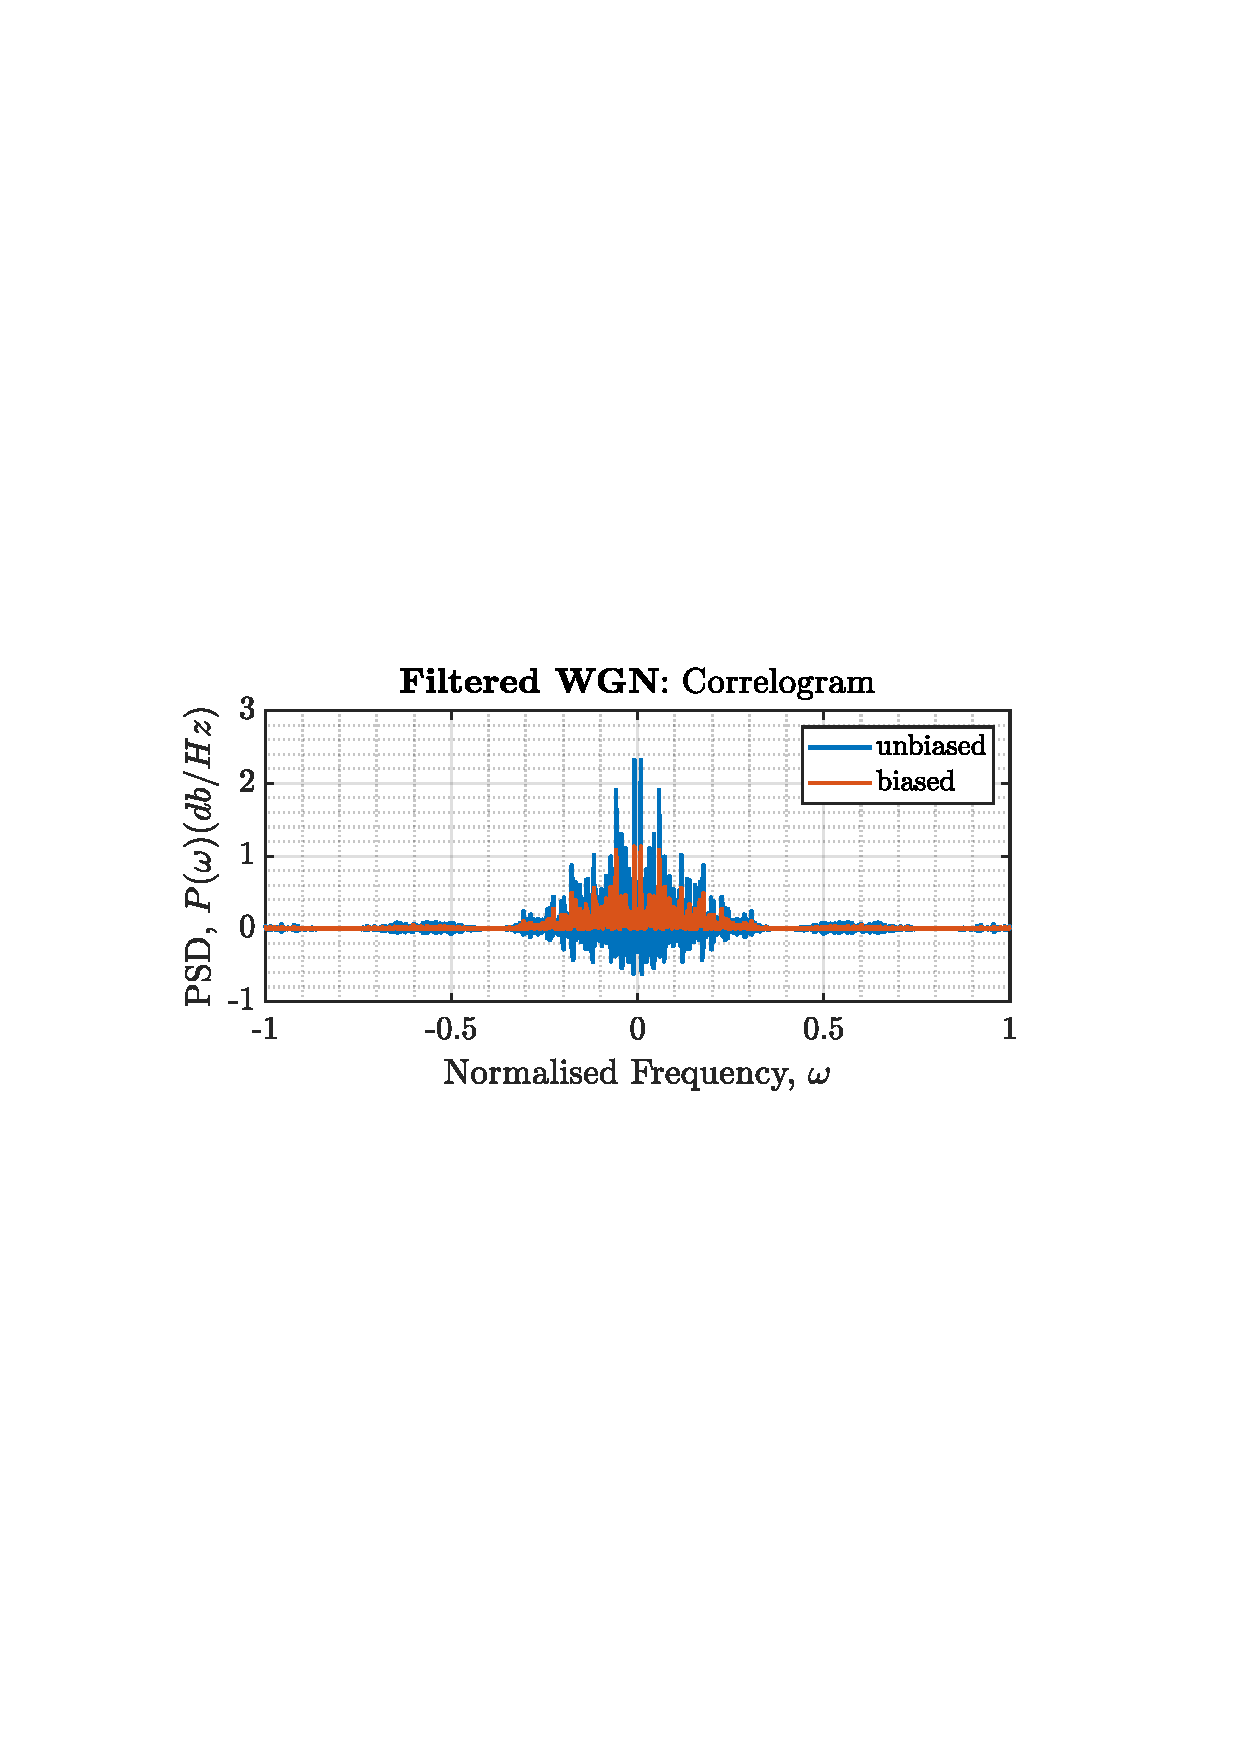
\includegraphics[trim={2.2cm 11.2cm 3.15cm  11.2cm}, clip, width=\textwidth]{../MATLAB/figures/q1_3a_fig05.pdf} 
		\end{subfigure}
		%		~ % forces onto the same row
		\begin{subfigure}{0.49\textwidth}
			\centering
			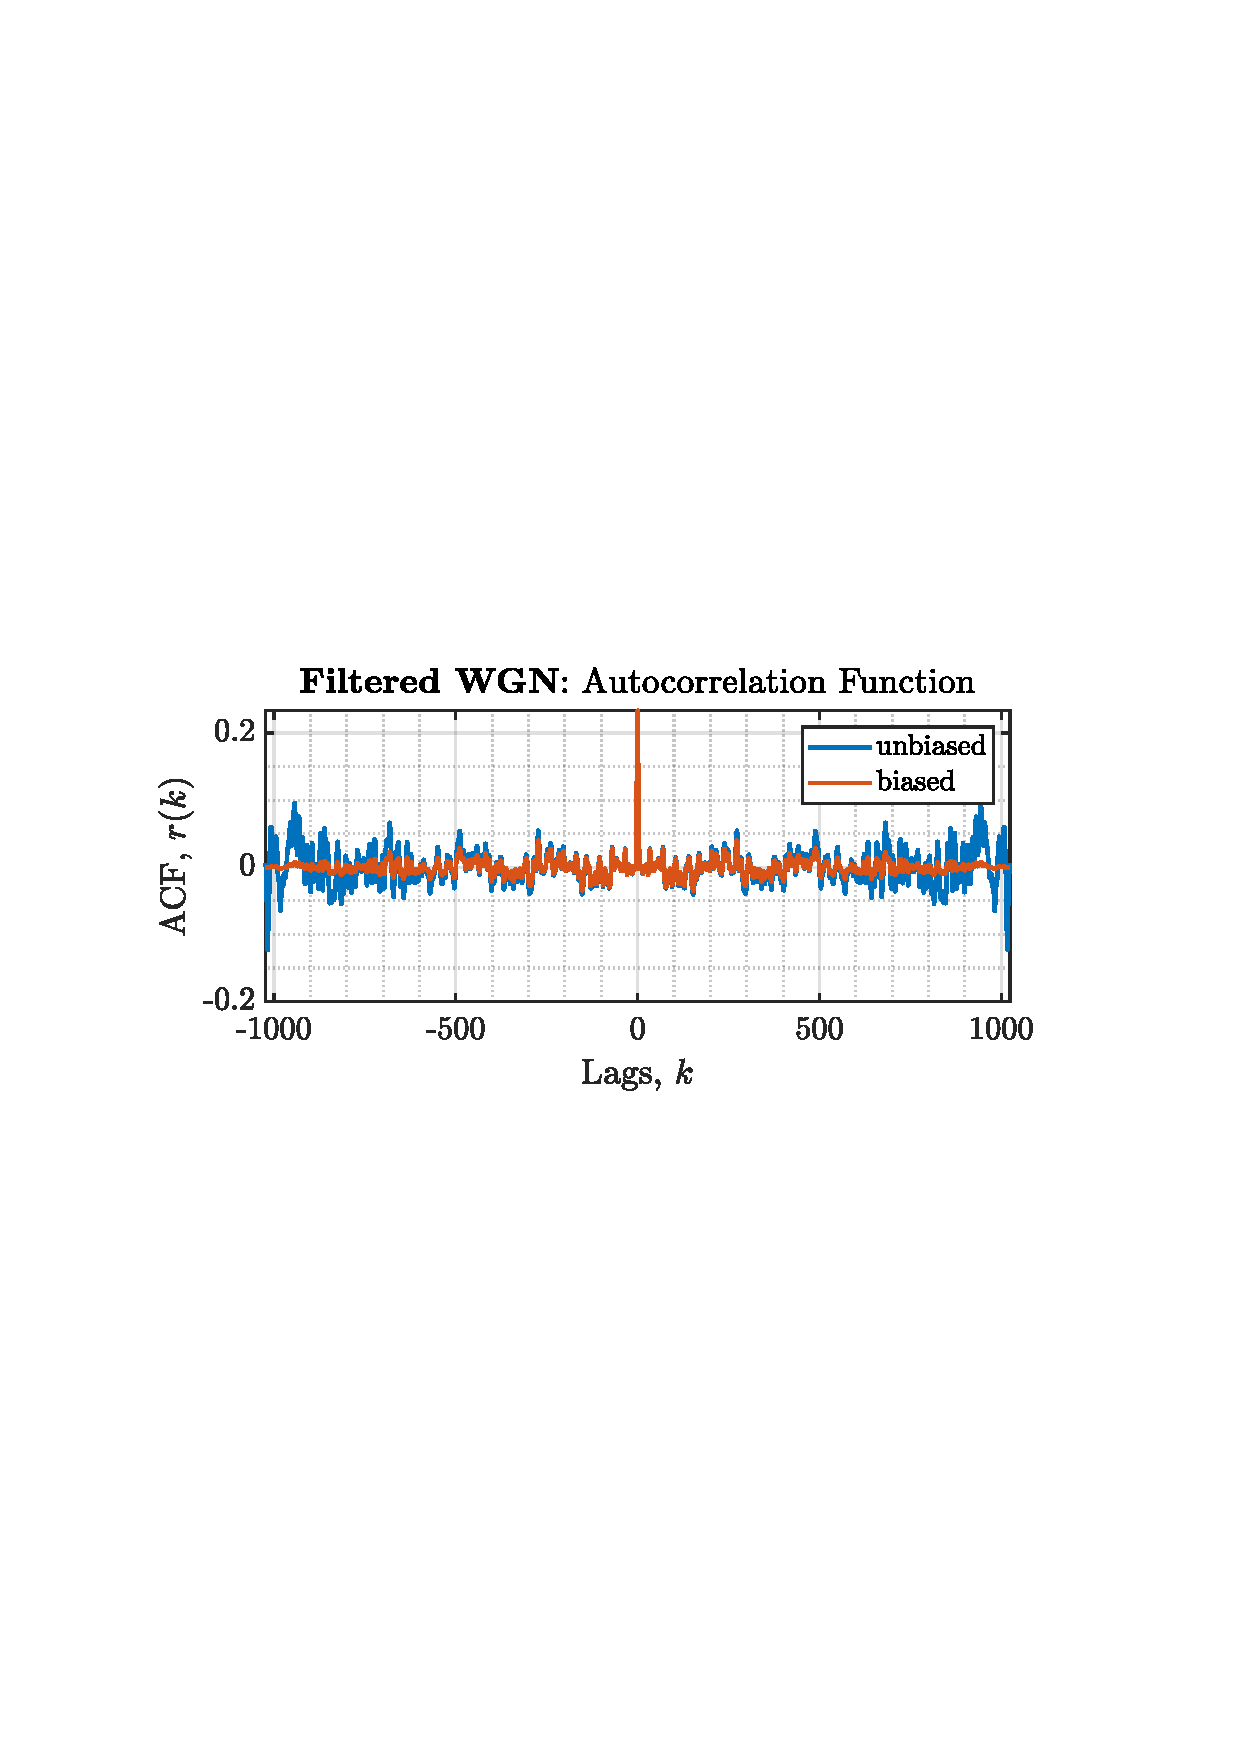
\includegraphics[trim={2.2cm 11.2cm 3.15cm  11.2cm}, clip, width=\textwidth]{../MATLAB/figures/q1_3a_fig06.pdf} 
		\end{subfigure}
		\captionsetup{justification=centering}
		\caption{Set of Auto-Correlation Functions (ACFs) and their Correlograms}
		\label{fig: 1-3a}
	\end{figure}

	\subsubsection{Biased ACF Estimator PSDs}

	\begin{figure}[H]
		\centering
		\begin{subfigure}{0.49\textwidth}
			\centering
			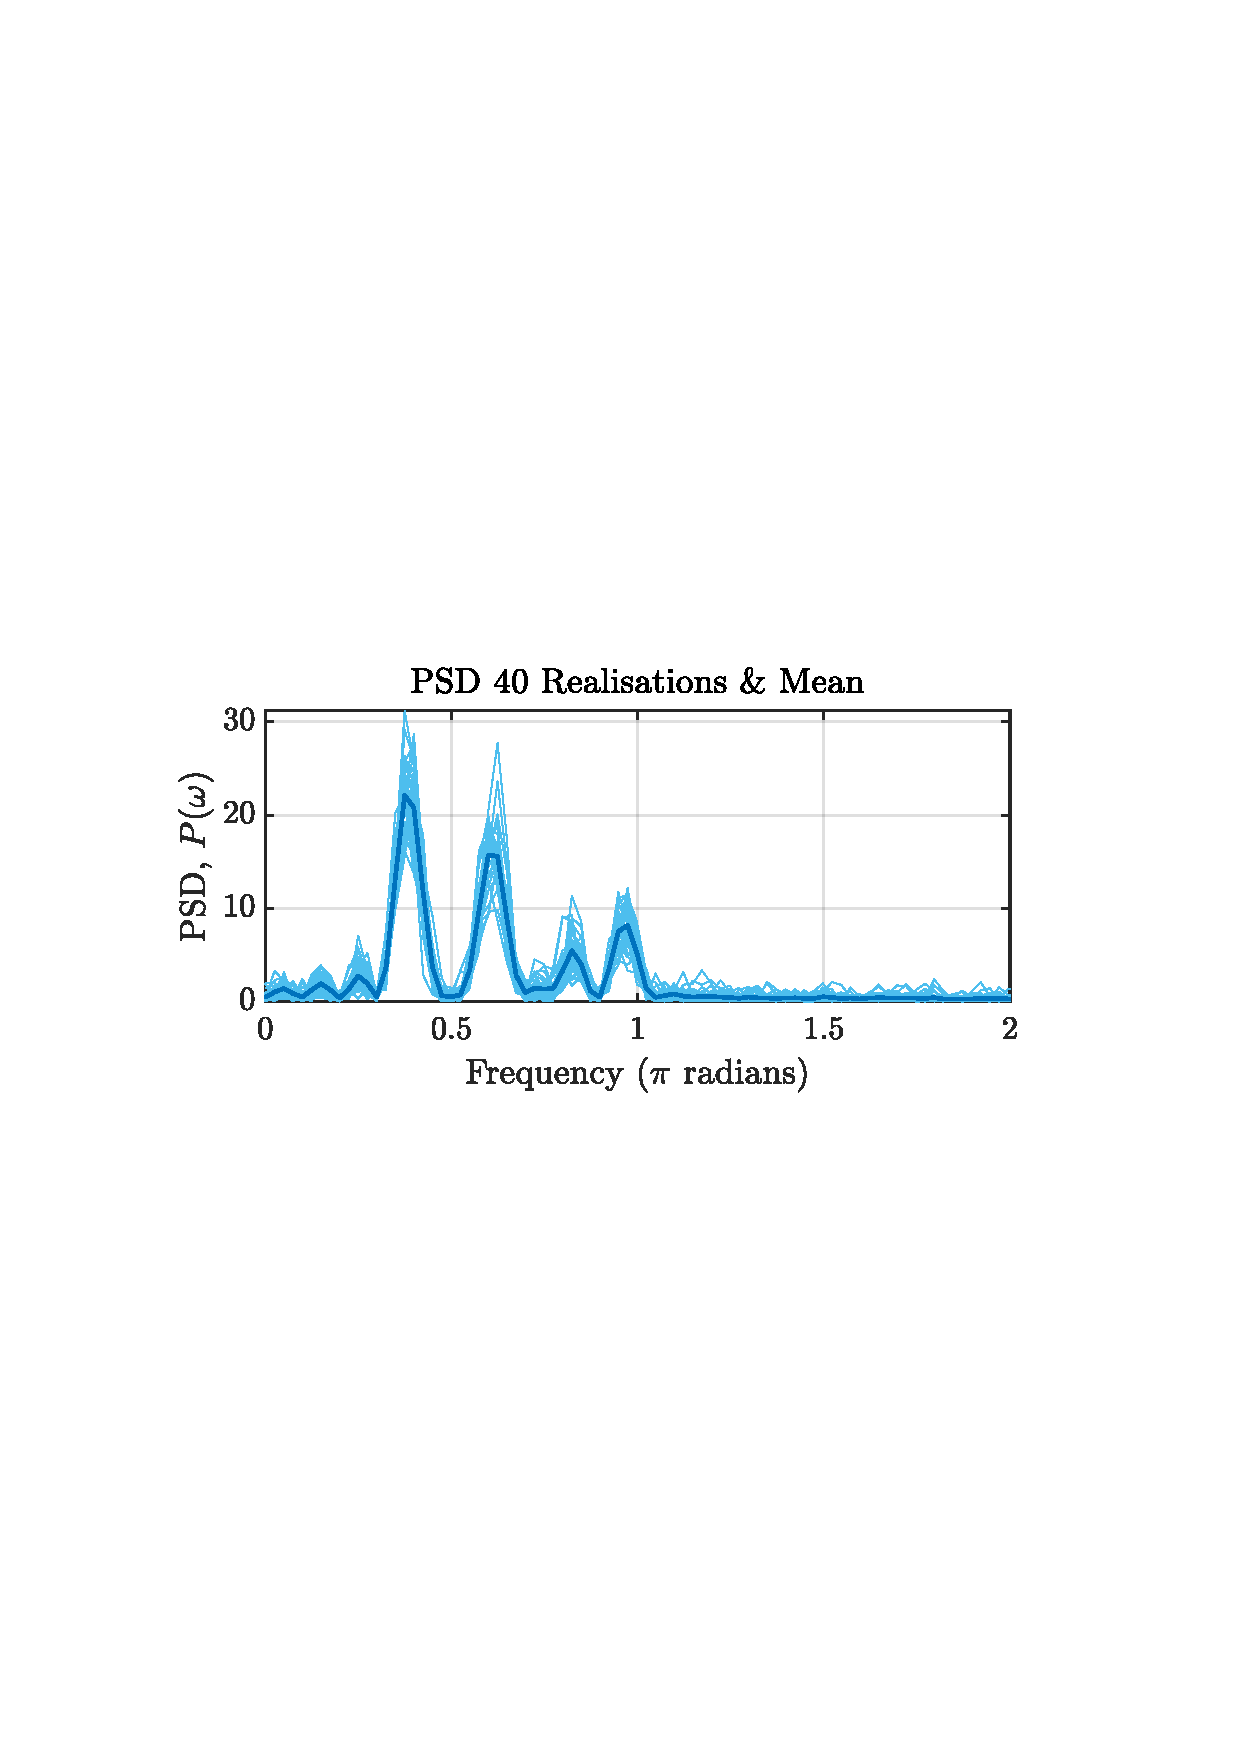
\includegraphics[trim={2.2cm 11.2cm 3.15cm  11.2cm}, clip, width=\textwidth]{../MATLAB/figures/q1_3b_fig01.pdf} 
			\captionsetup{justification=centering}
			\caption{Periodogram}
		\end{subfigure}
		%		~ % forces onto the same row
		\begin{subfigure}{0.49\textwidth}
			\centering
			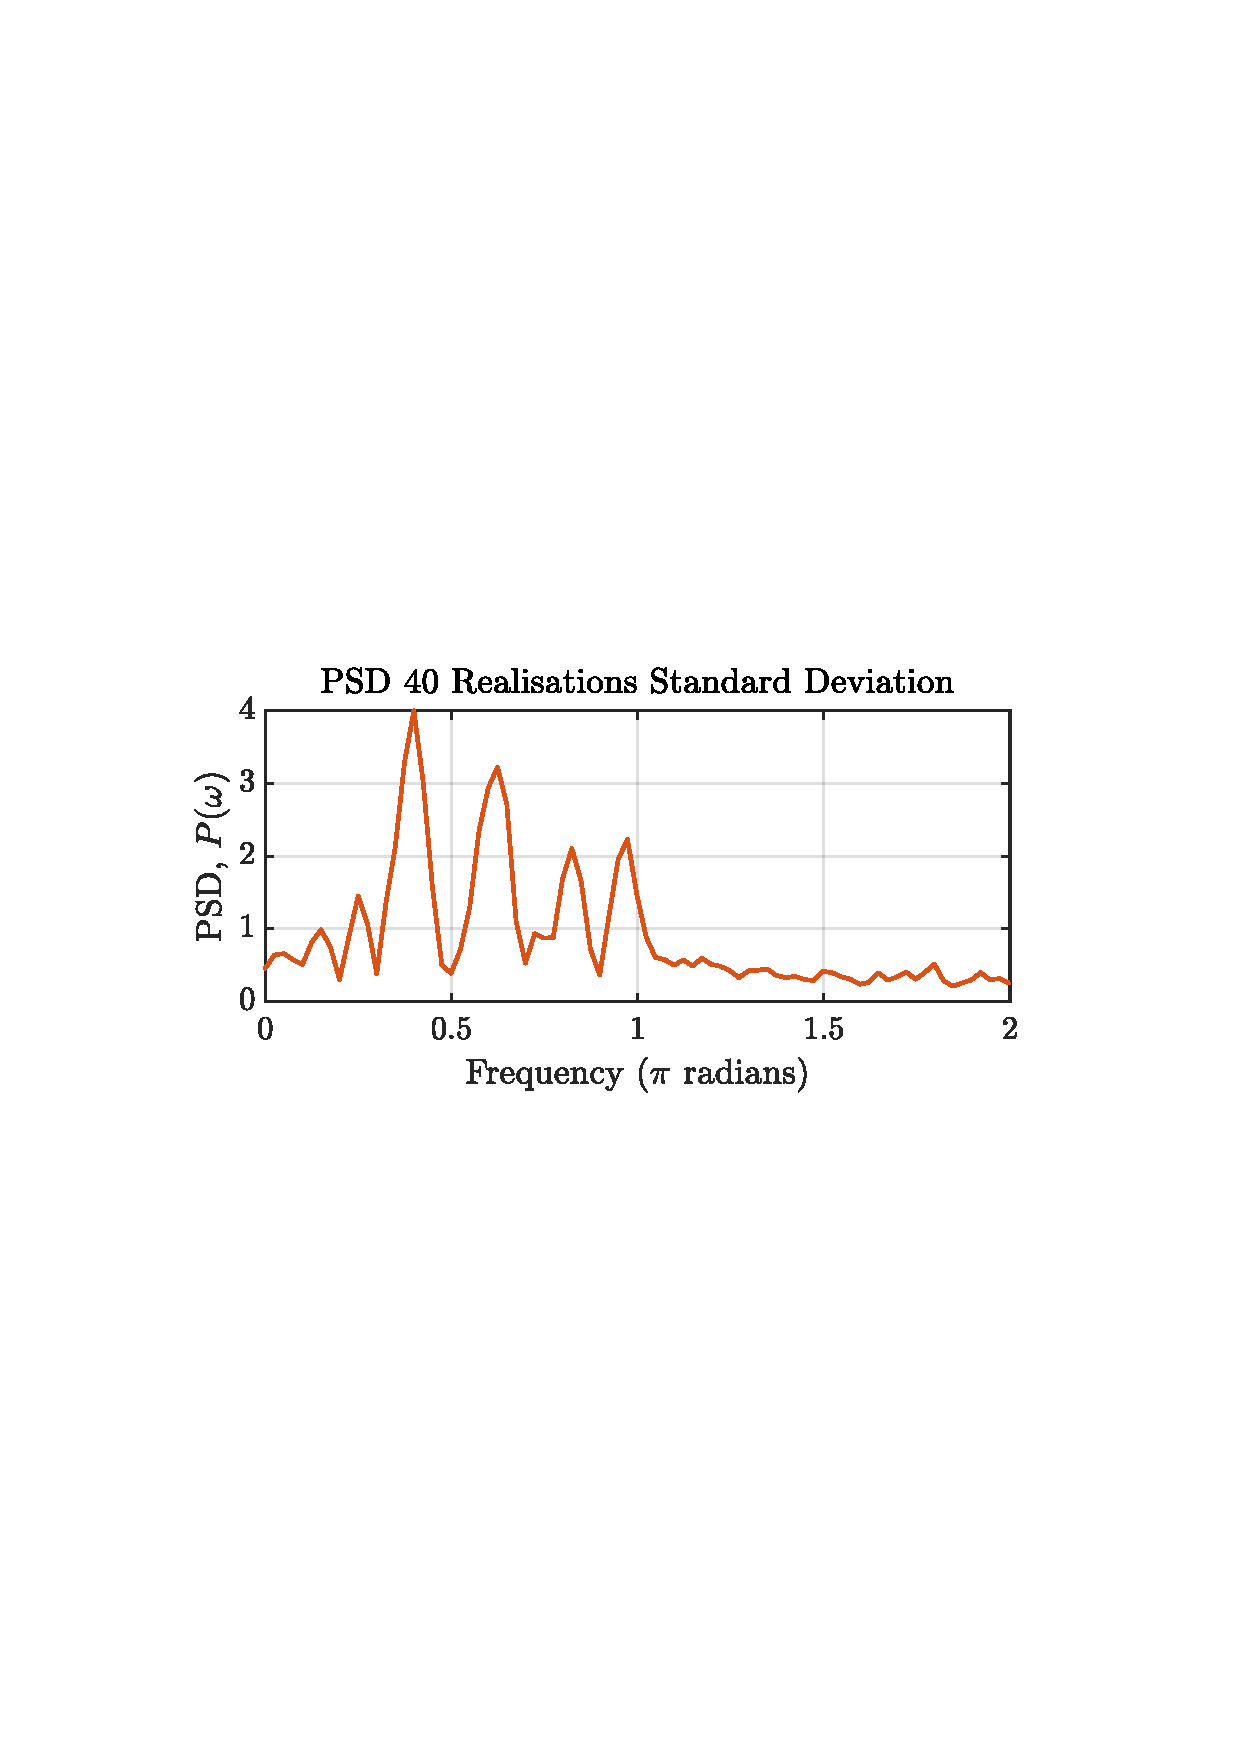
\includegraphics[trim={2.2cm 11.2cm 3.15cm  11.2cm}, clip, width=\textwidth]{../MATLAB/figures/q1_3b_fig02.pdf} 
			\captionsetup{justification=centering}
			\caption{Standard Deviation}
		\end{subfigure}
		\label{fig: 1-3b}
	\end{figure}

	\subsubsection{Biased ACF Estimator PSDs on the dB Scale}
	% TODO: Make vertical lines at the frequencies of your function
	\begin{figure}[H]
		\centering
		\begin{subfigure}{0.49\textwidth}
			\centering
			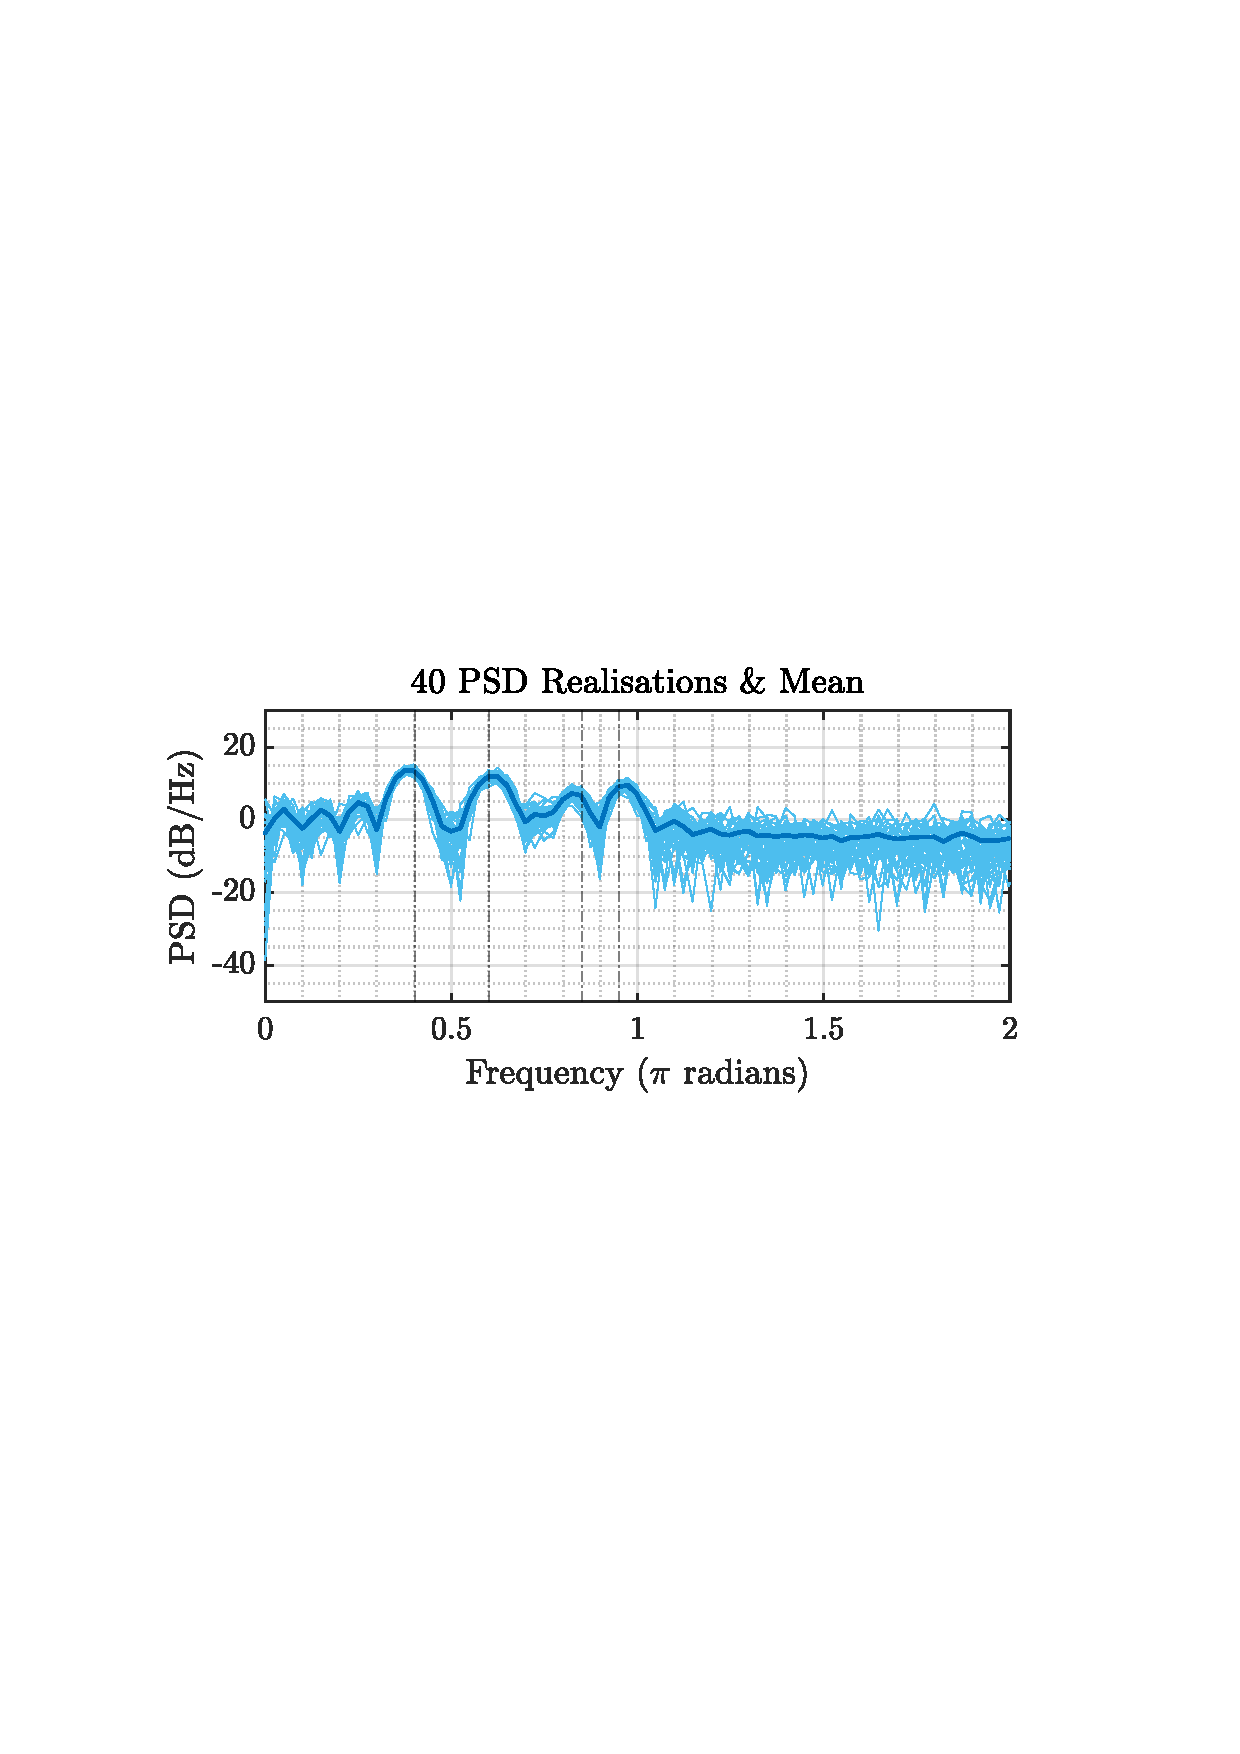
\includegraphics[trim={2.2cm 11.2cm 3.15cm  11.2cm}, clip, width=\textwidth]{../MATLAB/figures/q1_3c_fig01.pdf} 
			\captionsetup{justification=centering}
			\caption{Periodogram}
		\end{subfigure}
		%		~ % forces onto the same row
		\begin{subfigure}{0.49\textwidth}
			\centering
			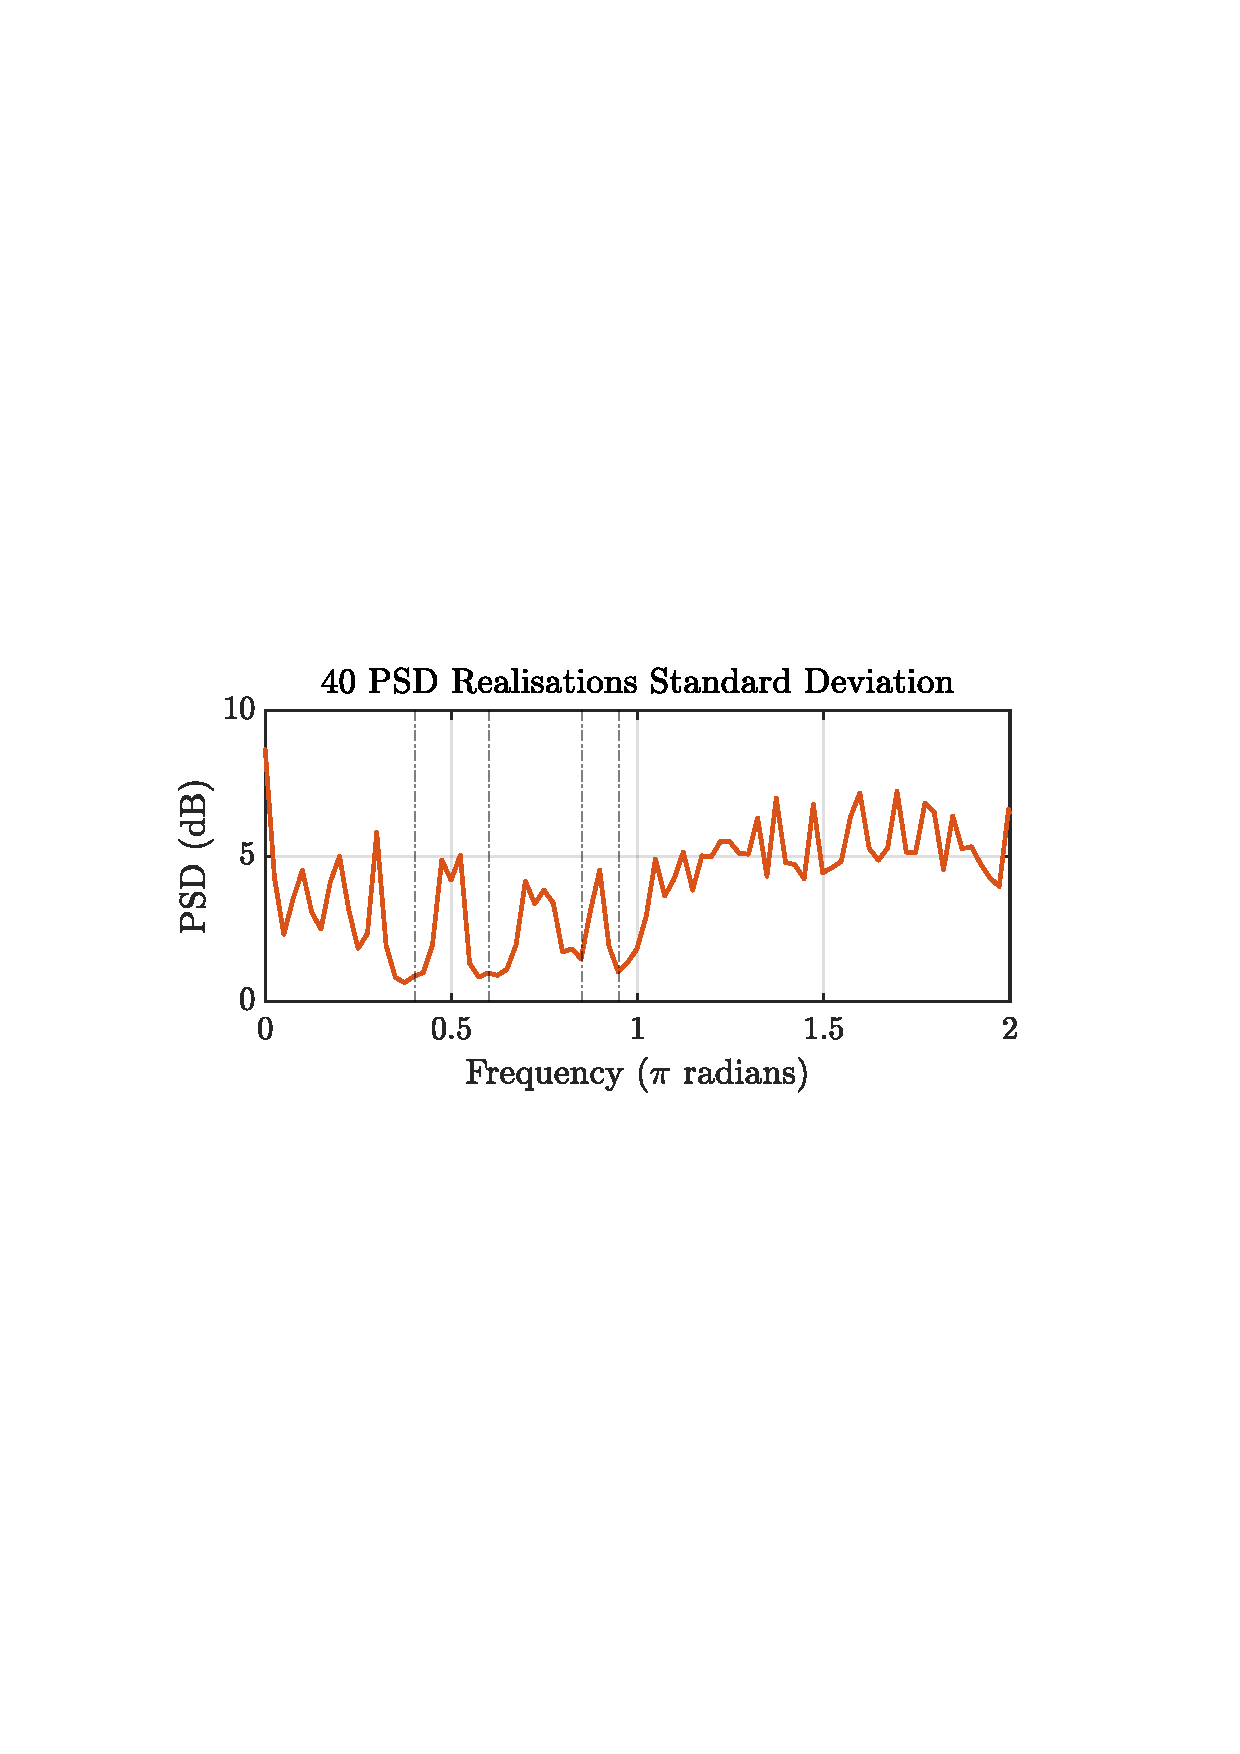
\includegraphics[trim={2.2cm 11.2cm 3.15cm  11.2cm}, clip, width=\textwidth]{../MATLAB/figures/q1_3c_fig02.pdf} 
			\captionsetup{justification=centering}
			\caption{Standard Deviation}
		\end{subfigure}
		\label{fig: 1-3c}
	\end{figure}

	\subsubsection{Influence of Data Samples on the PSD}
	
	\begin{figure}[H]
		\centering
		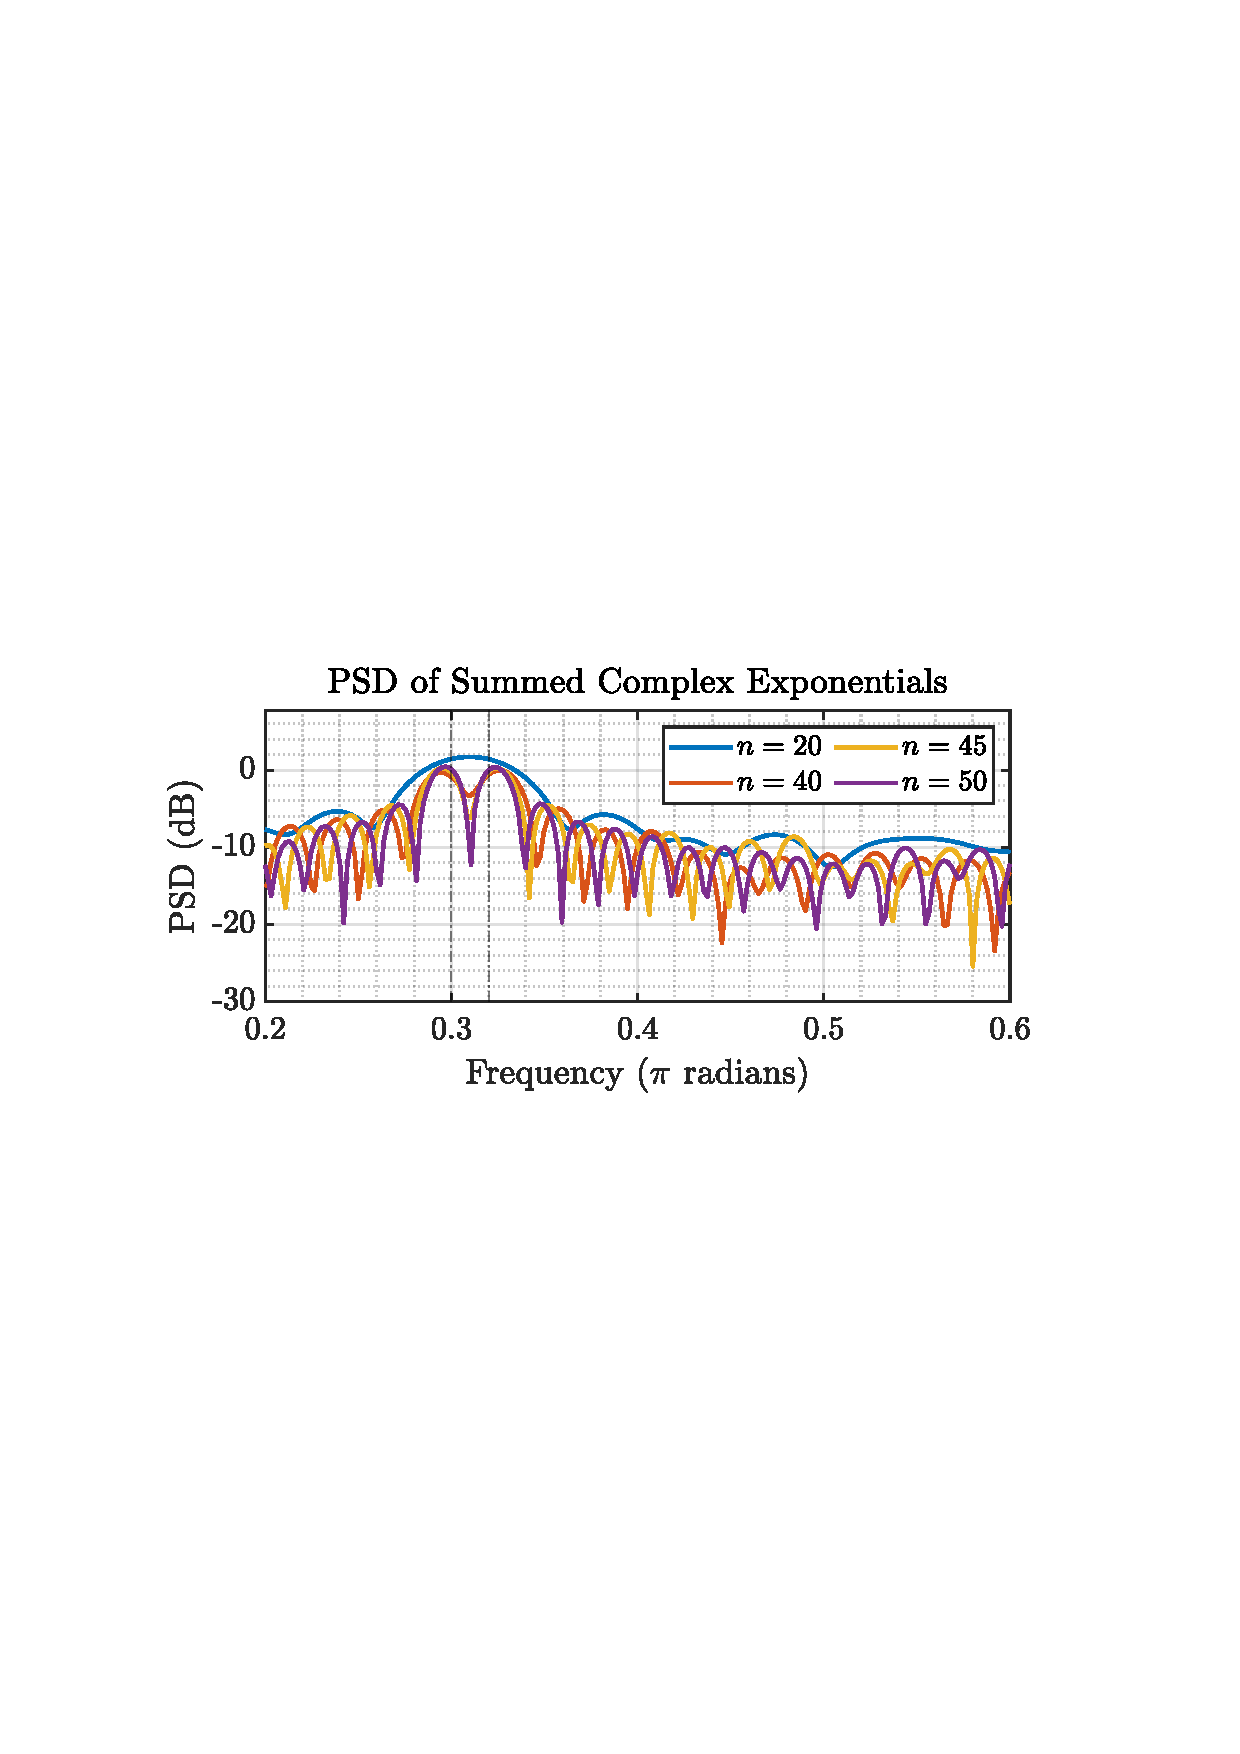
\includegraphics[trim={2.2cm 11.2cm 3.15cm  11.2cm}, clip, width=0.9\textwidth]{../MATLAB/figures/q1_3d_fig01.pdf} 
		\captionsetup{justification=centering}
		\caption{PSD while varying $n$, the number of Data Samples used}
		\label{fig: 1-3d}
	\end{figure}	
	
	\subsubsection{MUltiple SIgnal Classification (MUSIC) Estimator}
	
	\begin{figure}[H]
		\centering
		\begin{subfigure}{0.49\textwidth}
			\centering
			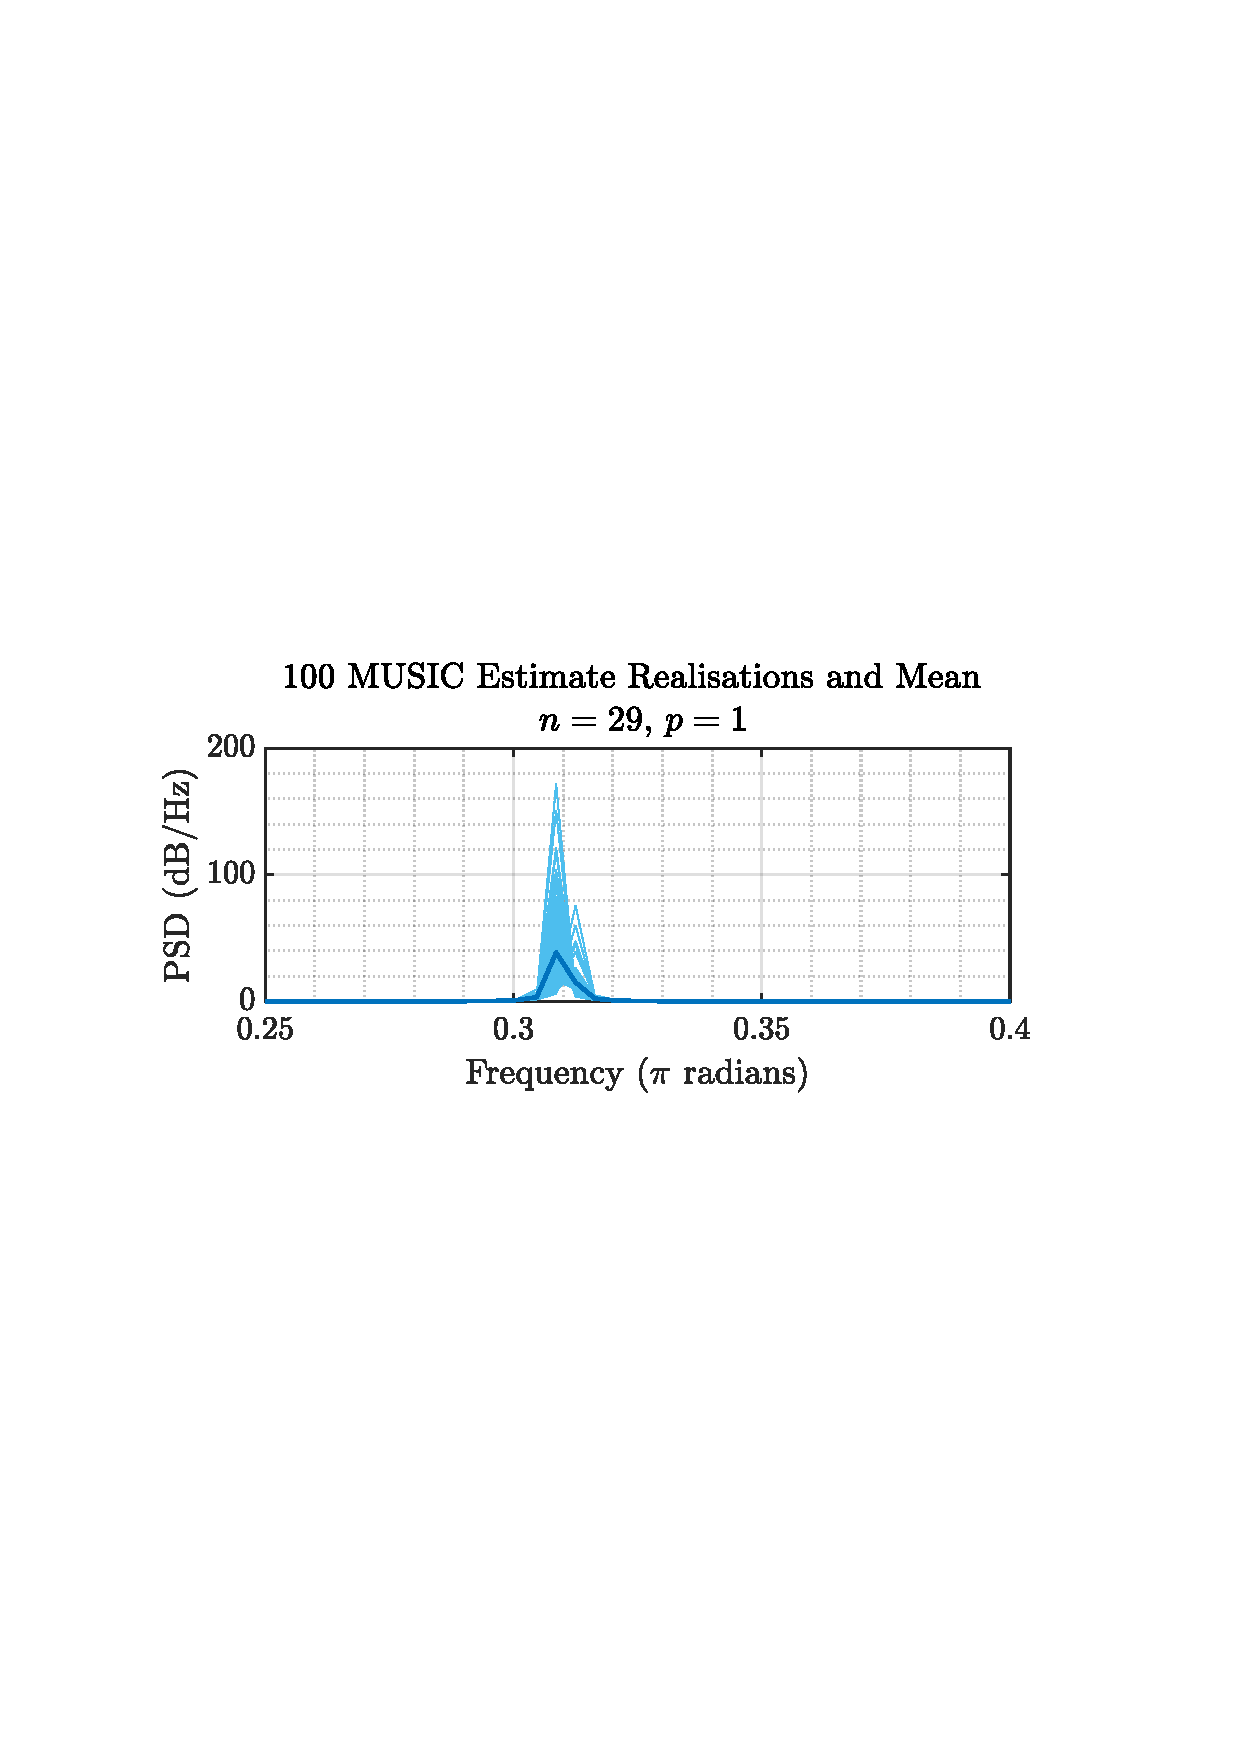
\includegraphics[trim={2.2cm 11cm 3.15cm  11.2cm}, clip, width=\textwidth]{../MATLAB/figures/q1_3e_fig01.pdf} 
		\end{subfigure}
		%		~ % forces onto the same row
		\begin{subfigure}{0.49\textwidth}
			\centering
			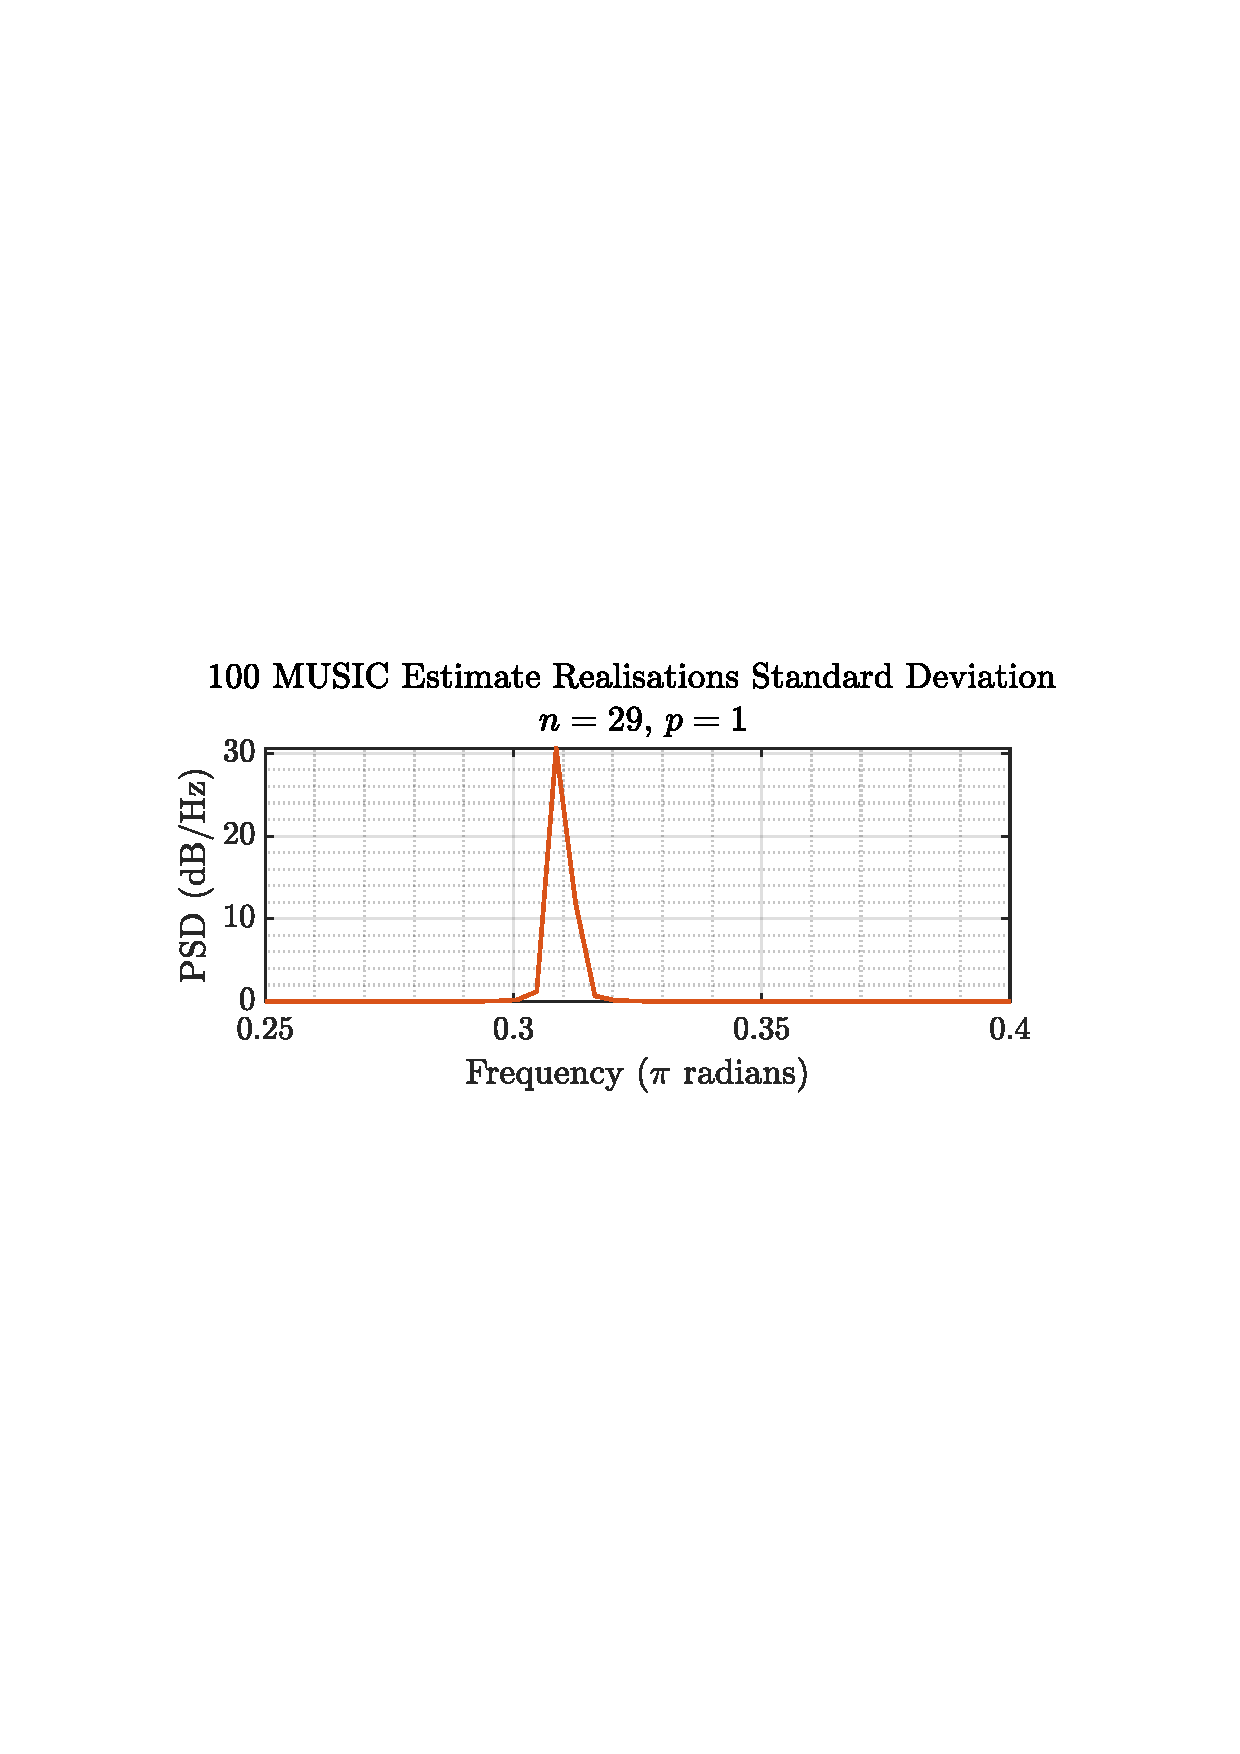
\includegraphics[trim={2.2cm 11cm 3.15cm  11.2cm}, clip, width=\textwidth]{../MATLAB/figures/q1_3e_fig02.pdf} 
		\end{subfigure}
		\begin{subfigure}{0.49\textwidth}
			\centering
			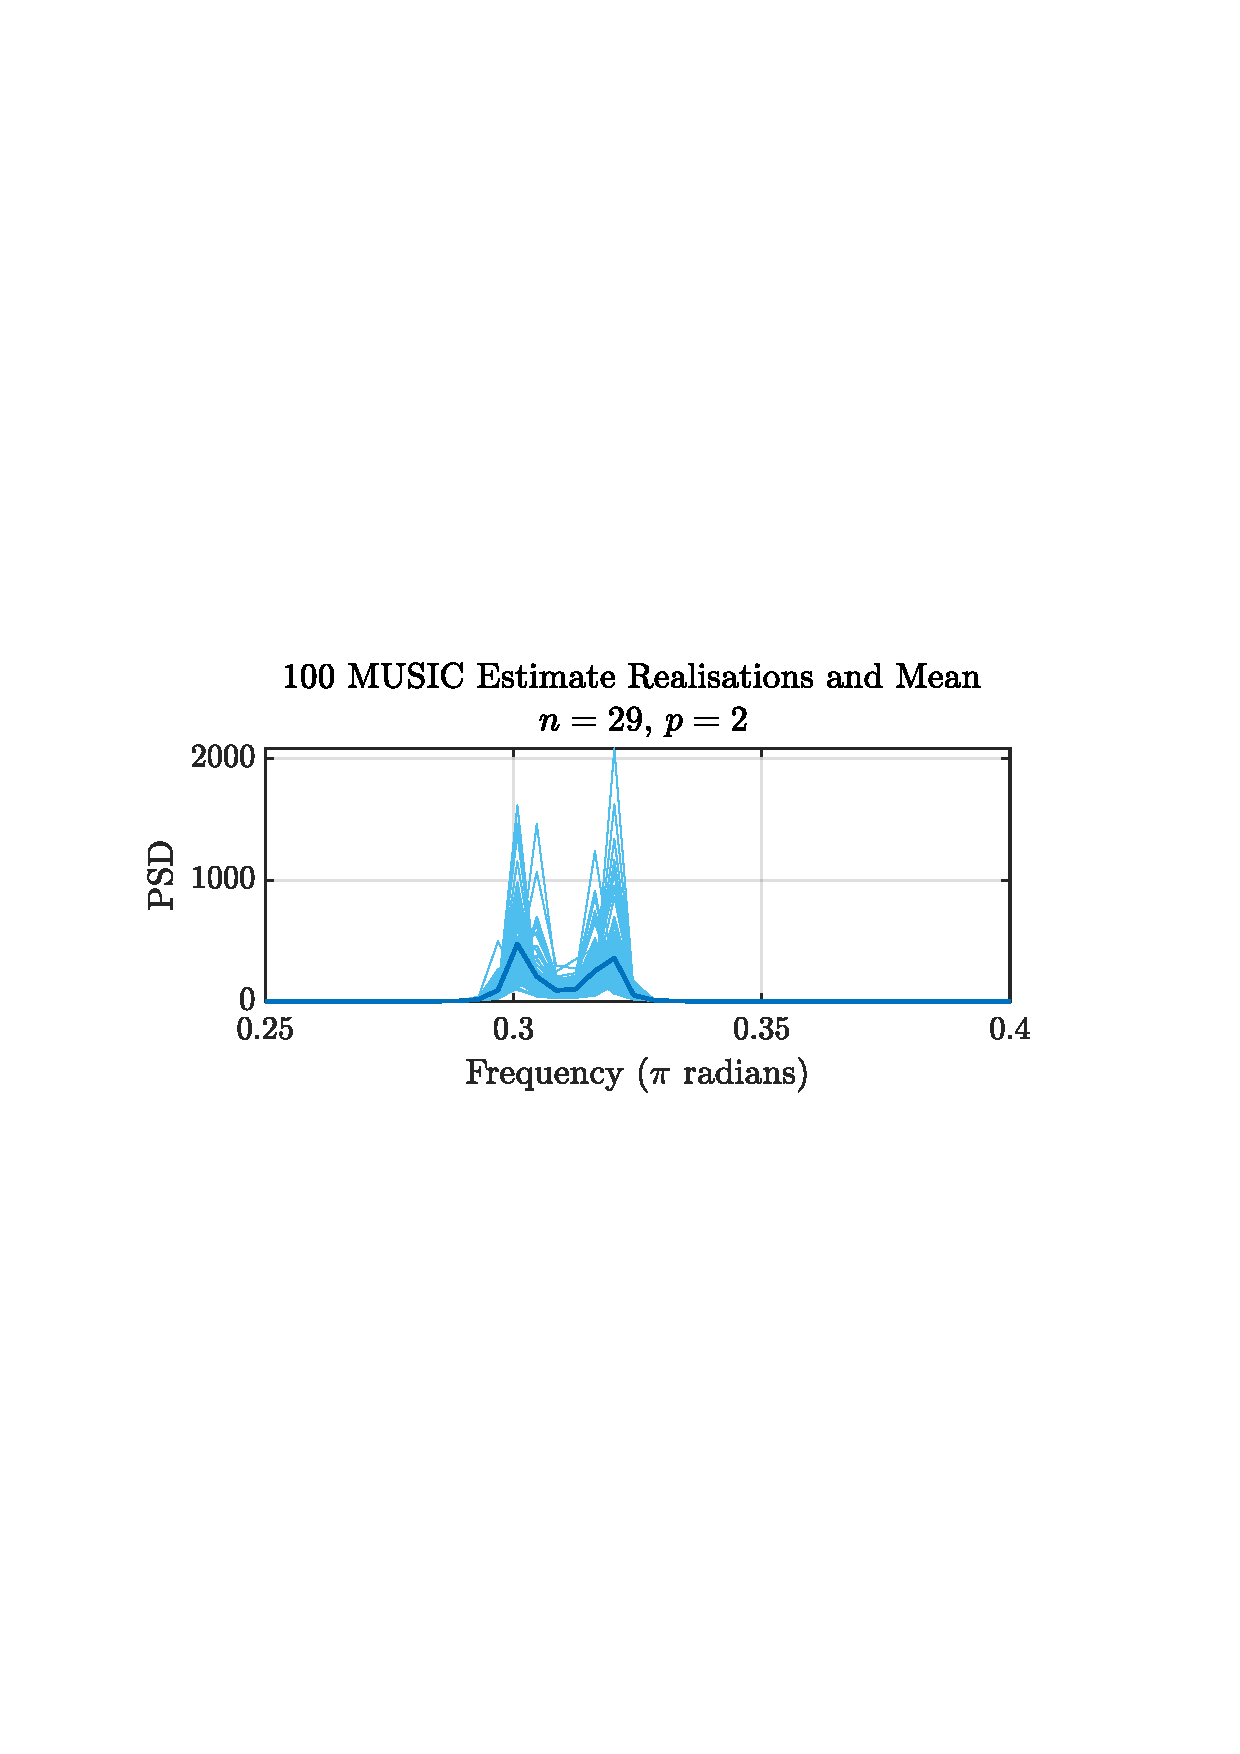
\includegraphics[trim={2.2cm 11cm 3.15cm  11.2cm}, clip, width=\textwidth]{../MATLAB/figures/q1_3e_fig03.pdf} 
		\end{subfigure}
		%		~ % forces onto the same row
		\begin{subfigure}{0.49\textwidth}
			\centering
			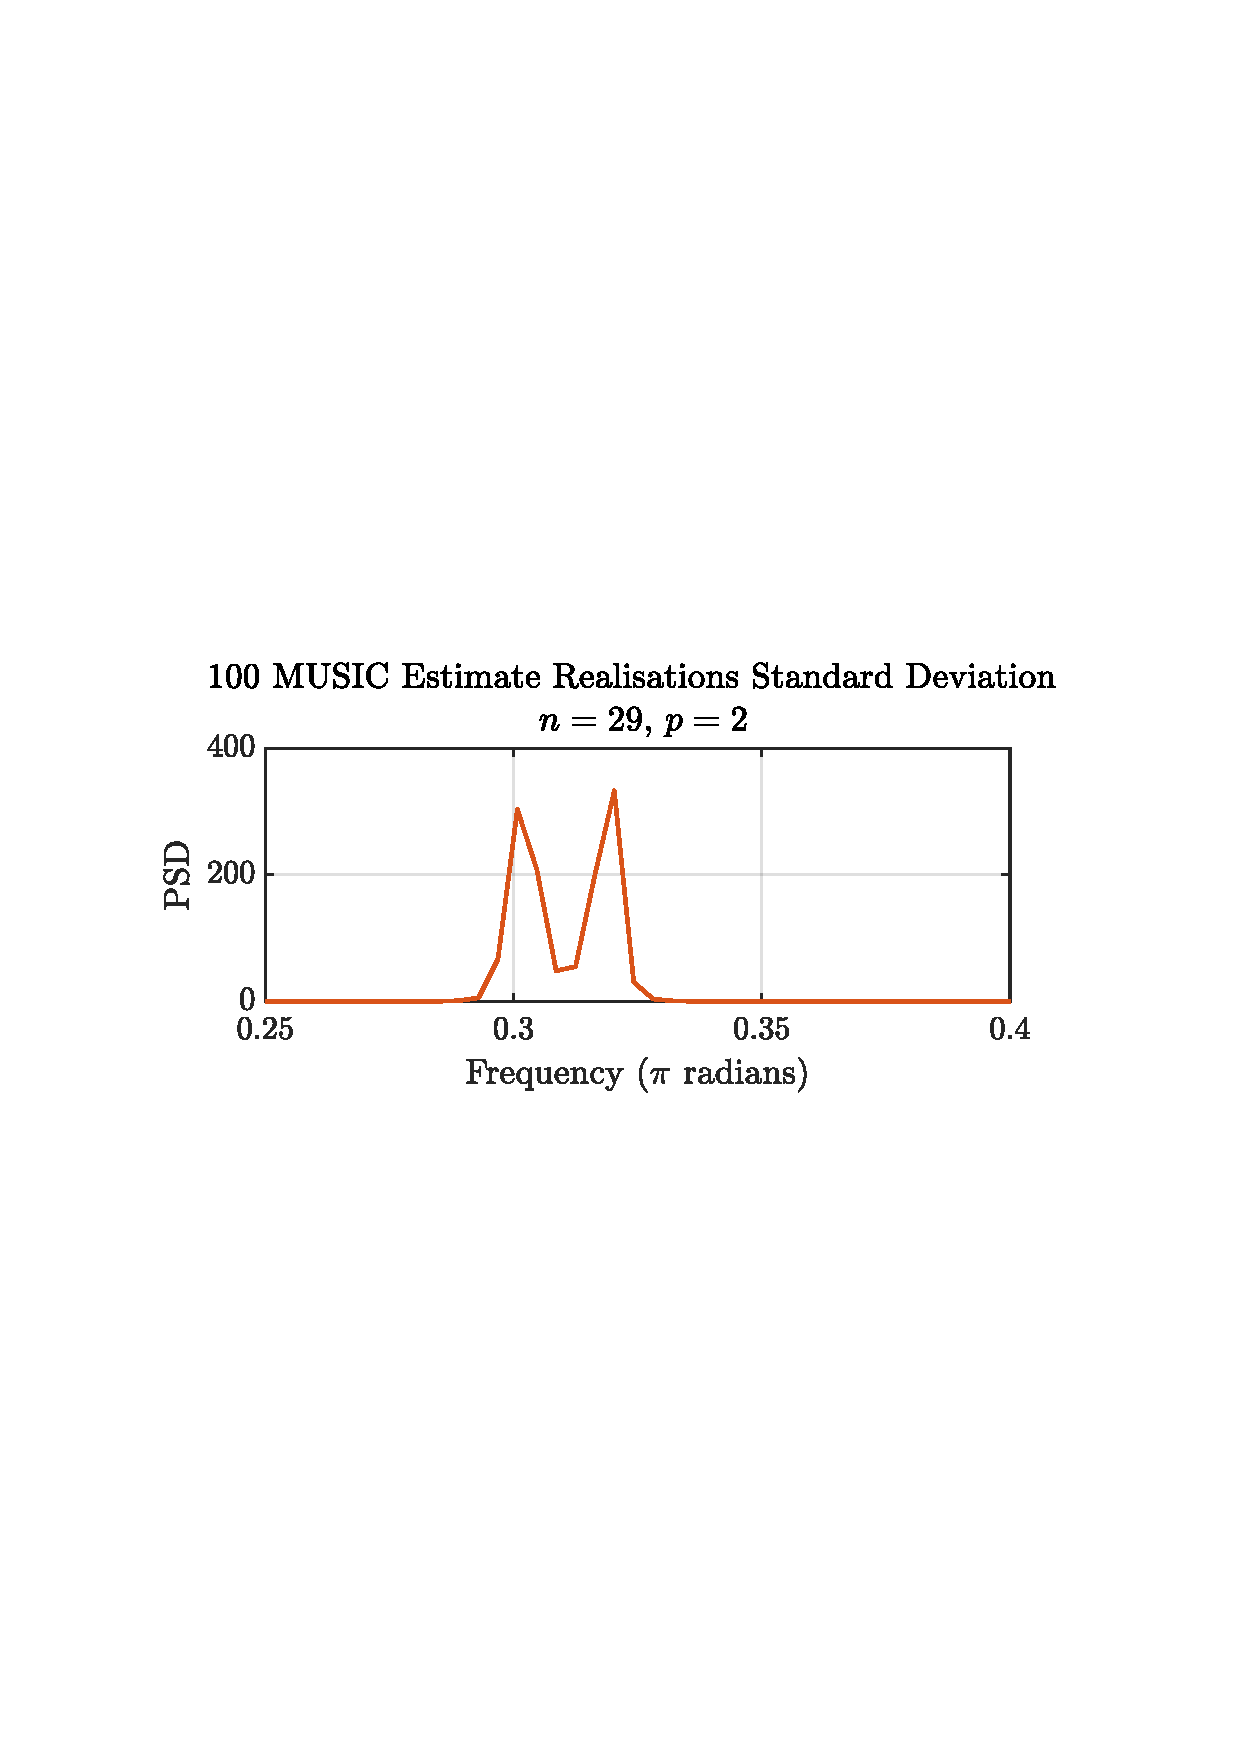
\includegraphics[trim={2.2cm 11cm 3.15cm  11.2cm}, clip, width=\textwidth]{../MATLAB/figures/q1_3e_fig04.pdf} 
		\end{subfigure}
		\begin{subfigure}{0.49\textwidth}
			\centering
			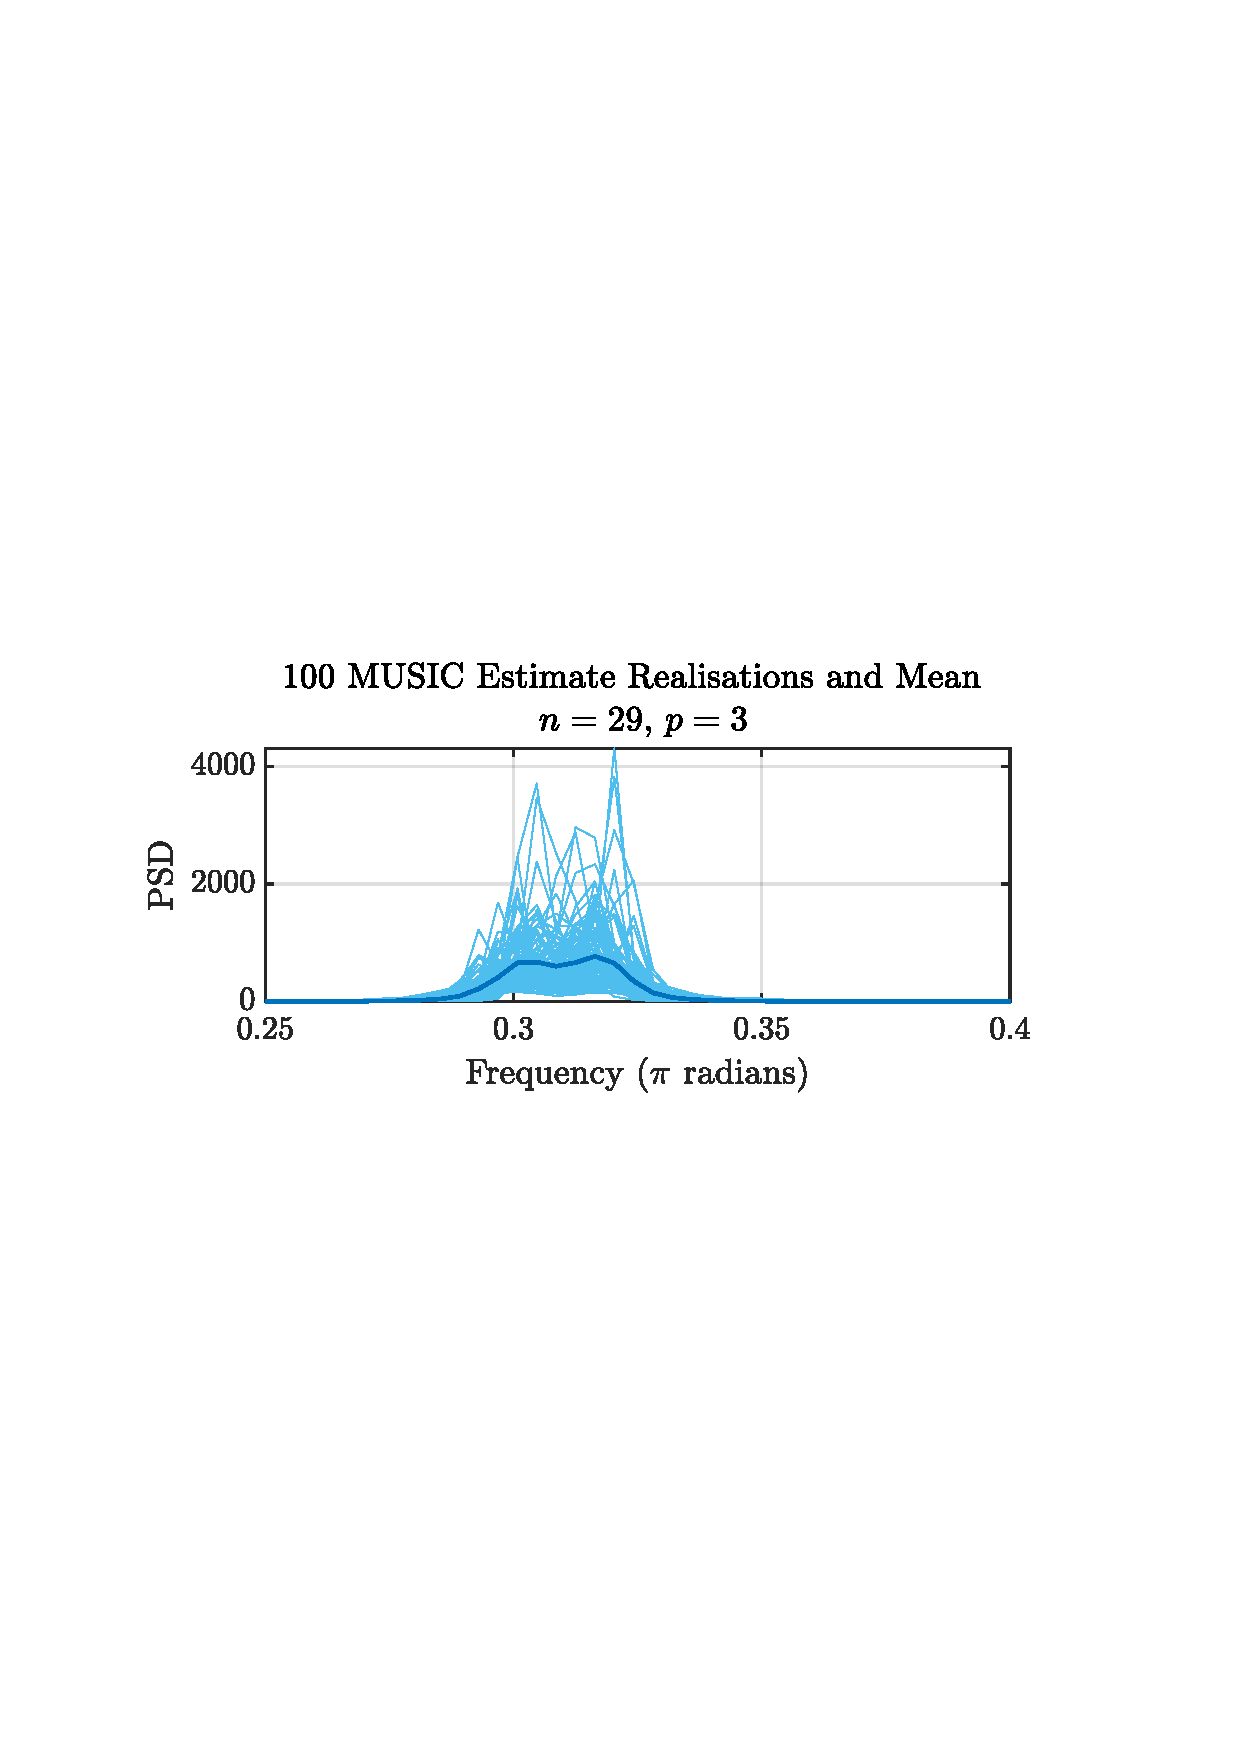
\includegraphics[trim={2.2cm 11.2cm 3.15cm  11.2cm}, clip, width=\textwidth]{../MATLAB/figures/q1_3e_fig05.pdf} 
		\end{subfigure}
		%		~ % forces onto the same row
		\begin{subfigure}{0.49\textwidth}
			\centering
			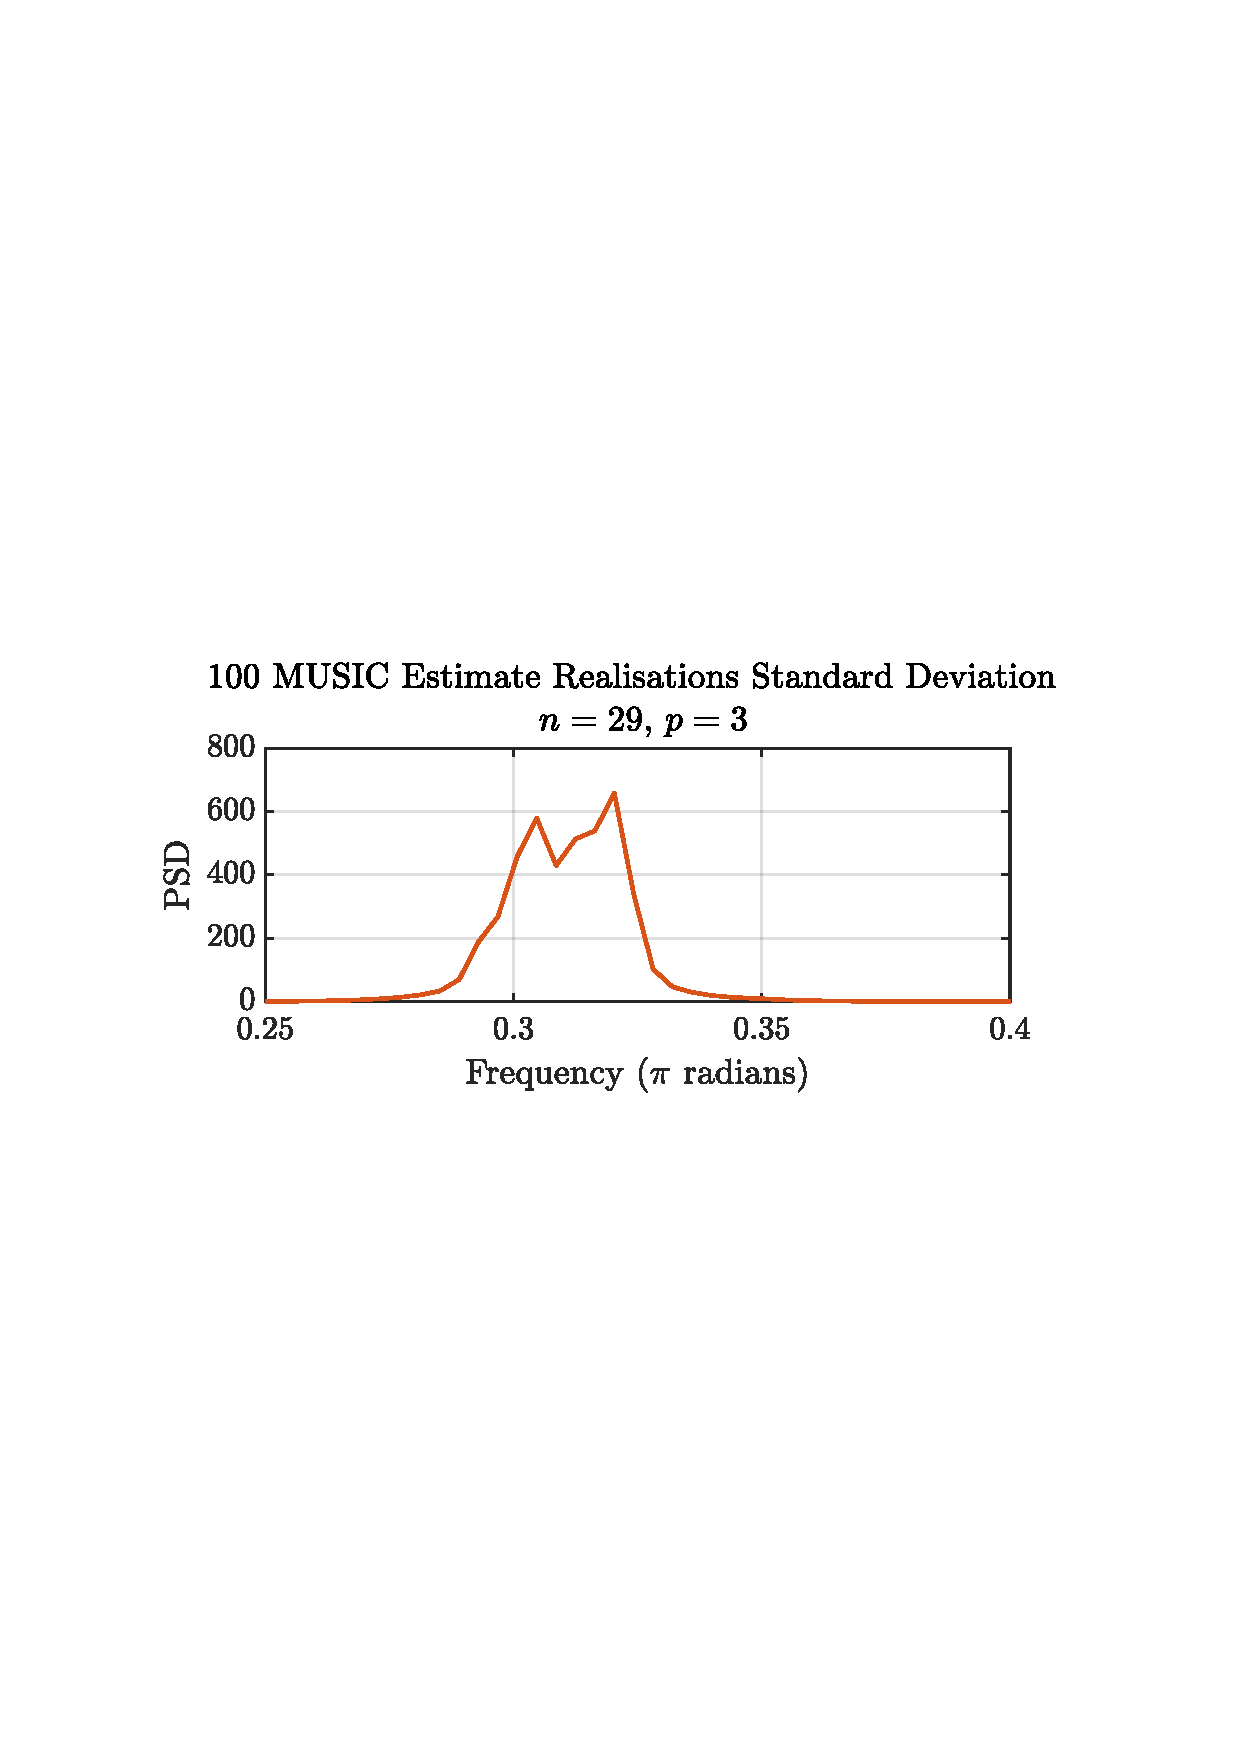
\includegraphics[trim={2.2cm 11.2cm 3.15cm  11.2cm}, clip, width=\textwidth]{../MATLAB/figures/q1_3e_fig06.pdf} 
		\end{subfigure}
		\captionsetup{justification=centering}
		\caption{Set of Auto-Correlation Functions (ACFs) and their Correlograms. \\ $n$ is the number of samples used, $p$ is the Signal Space Dimensionality}
		\label{fig: 1-3e}
	\end{figure}
	
	\subsection{Spectrum of Autoregressive (AR) Processes} \label{sec: 1-4-spectrums-AR}
	
	\subsubsection{Shortcomings of the Unbiased ACF in finding AR Parameters}
	
	\subsubsection{Error of the AR PSD Estimate}
	% TODO: BOTH b and c have AR(12) even though we show many orders
	\begin{figure}[H]
		\centering
		\begin{subfigure}{0.49\textwidth}
			\centering
			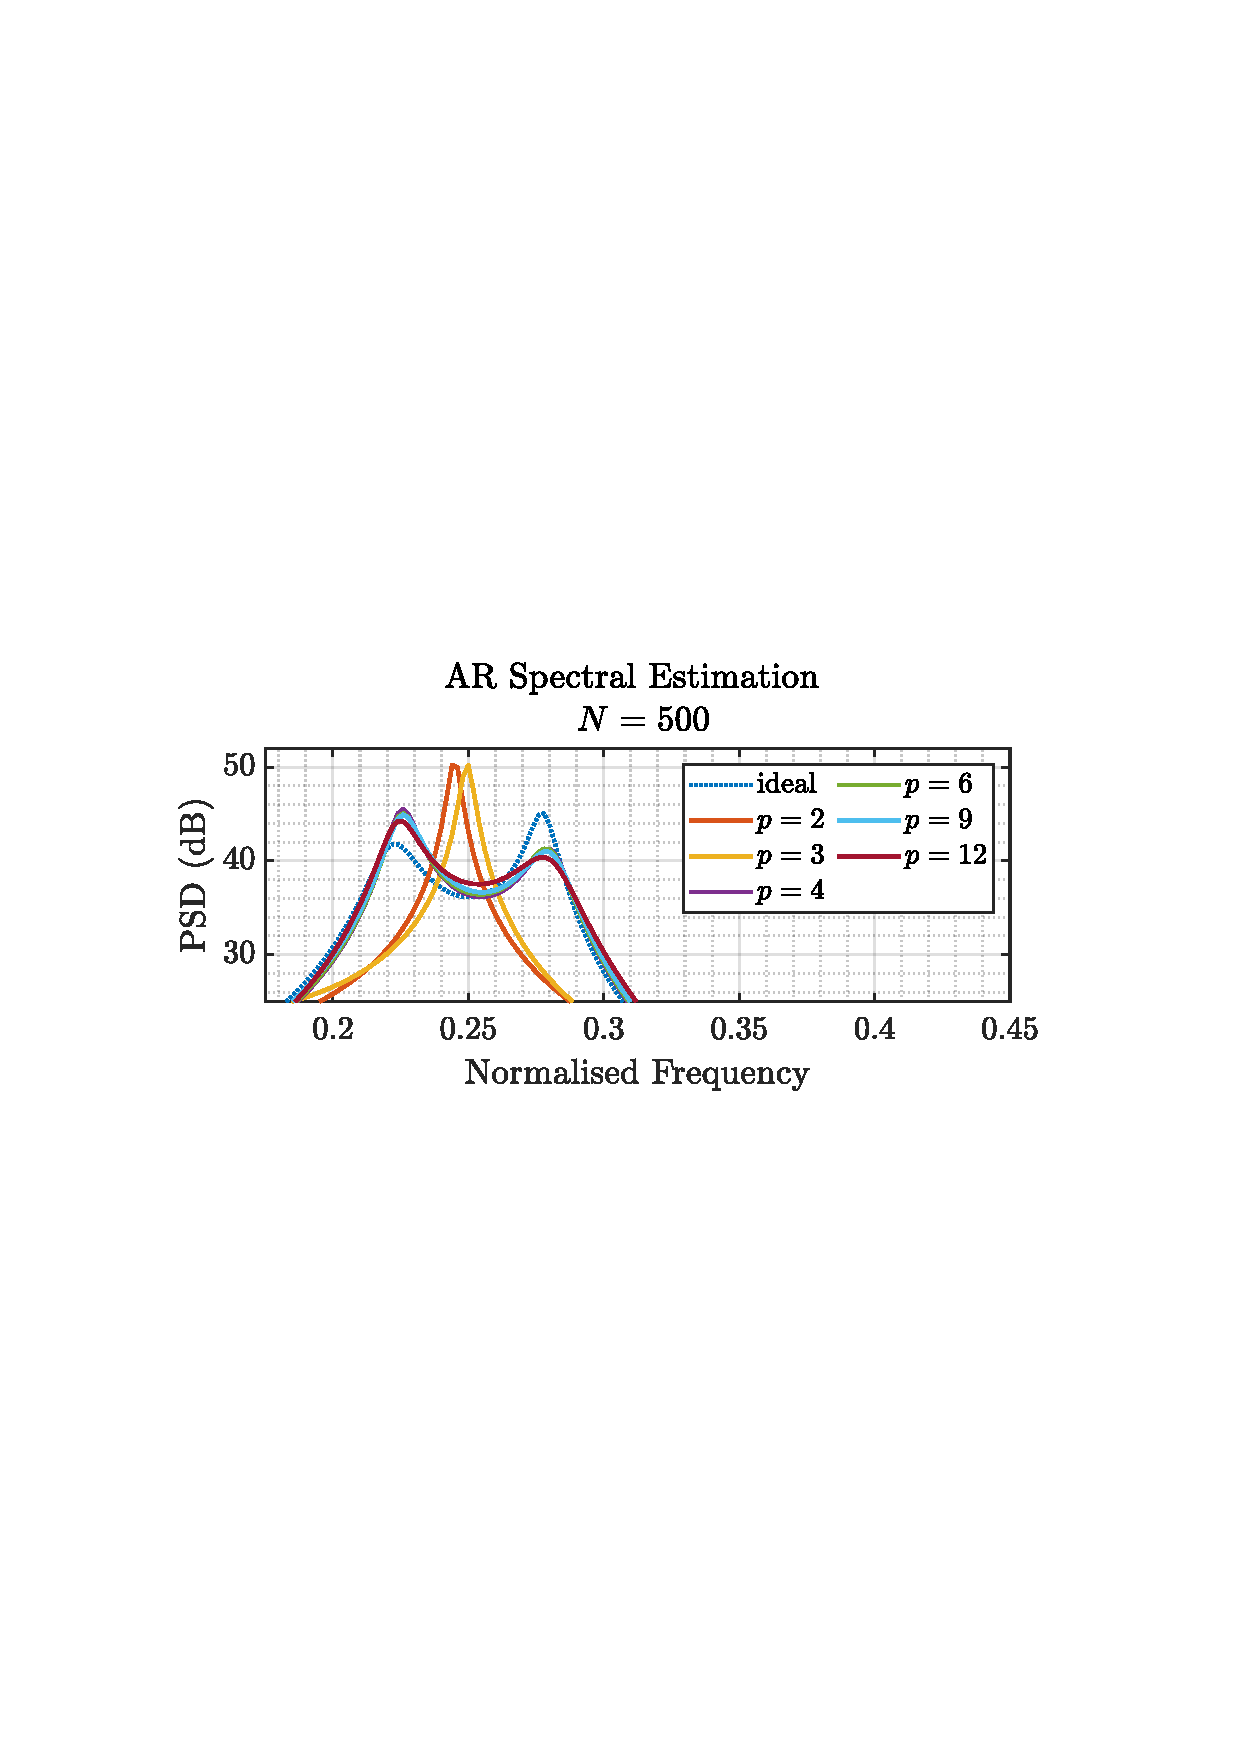
\includegraphics[trim={2.2cm 11.2cm 3.15cm  11.2cm}, clip, width=\textwidth]{../MATLAB/figures/q1_4b_fig14.pdf} 
			\captionsetup{justification=centering}
			\caption{AR Periodogram and its $p$ Order Estimates}
		\end{subfigure}
		%		~ % forces onto the same row
		\begin{subfigure}{0.49\textwidth}
			\centering
			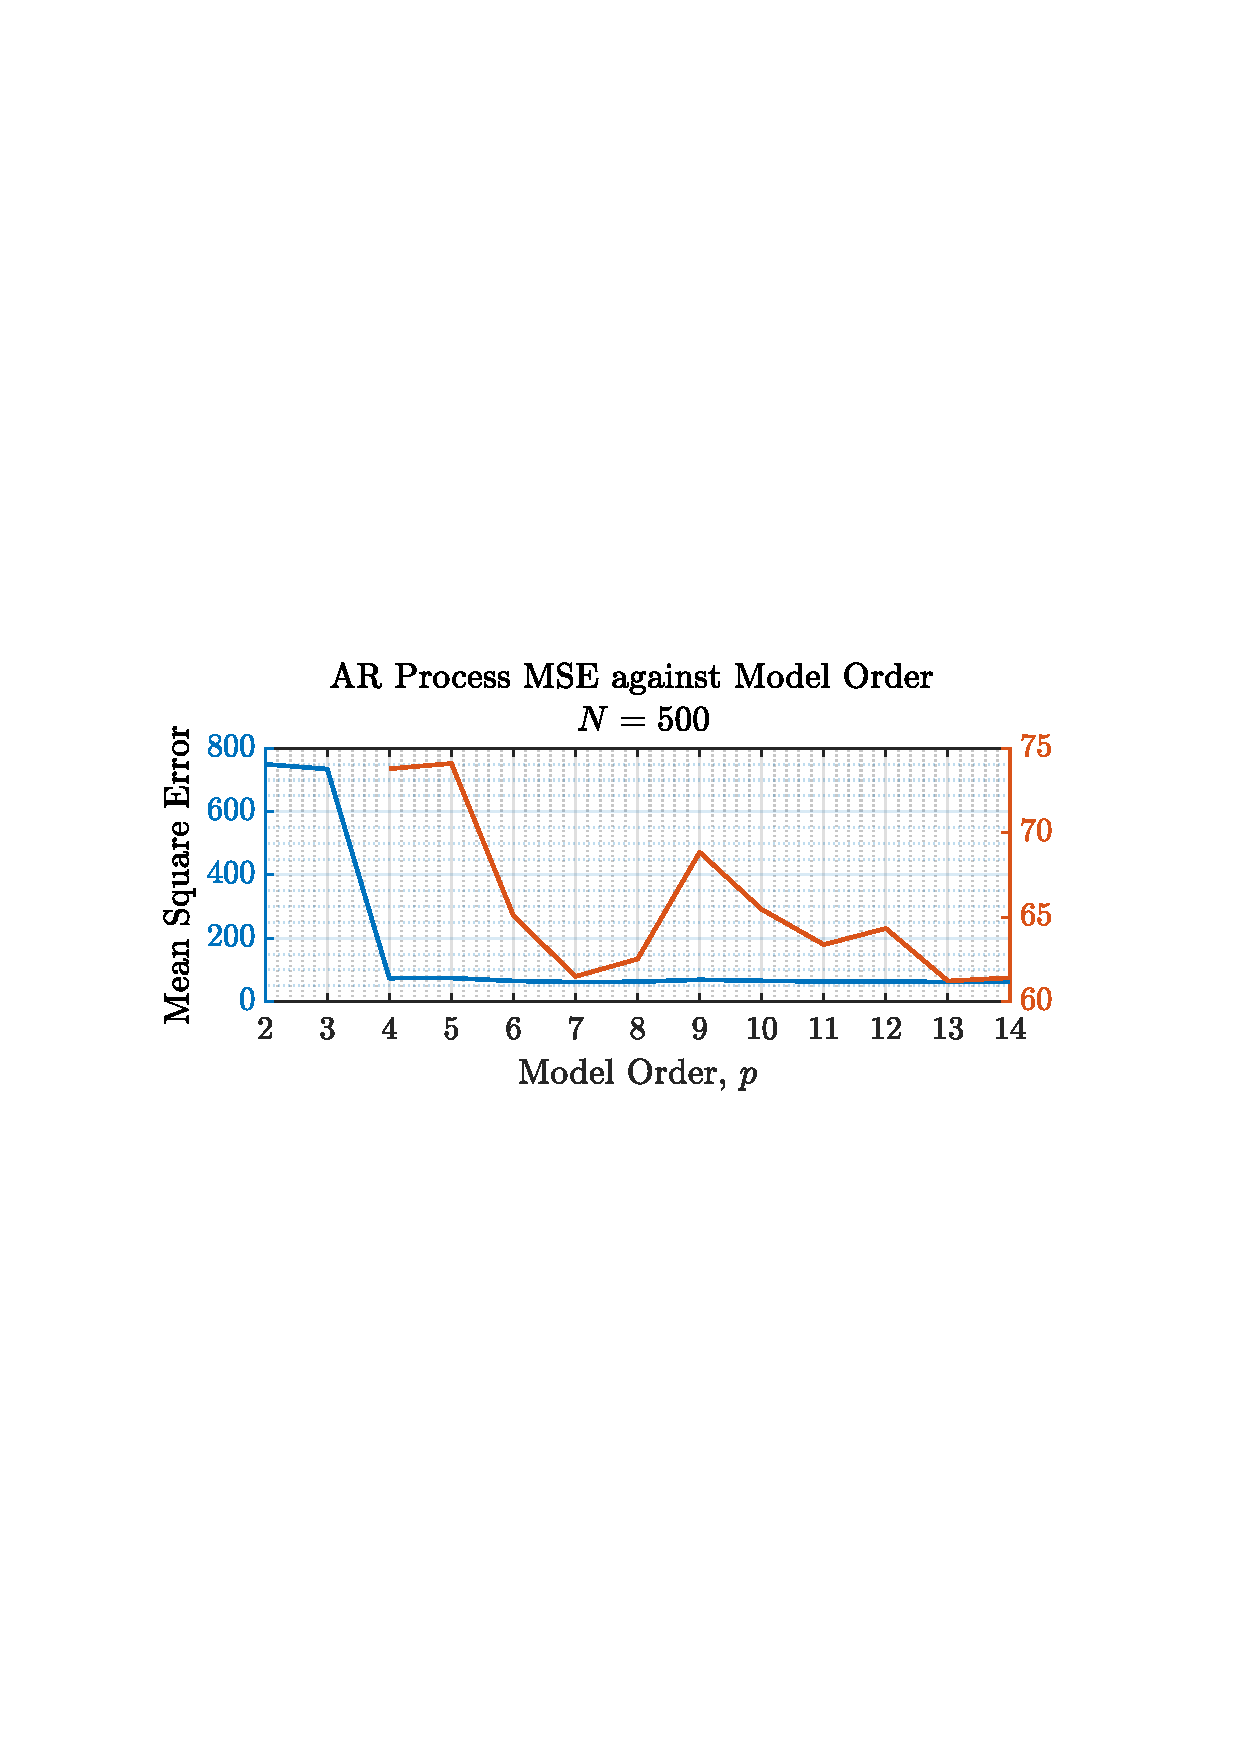
\includegraphics[trim={2.2cm 11.2cm 3.15cm  11.2cm}, clip, width=\textwidth]{../MATLAB/figures/q1_4b_fig16.pdf} 
			\captionsetup{justification=centering}
			\caption{Mean Squared Error}
		\end{subfigure}
		\label{fig: 1-4b}
	\end{figure}

	\subsubsection{Error of the AR PSD Estimate with more Samples}
	\begin{figure}[H]
		\centering
		\begin{subfigure}{0.49\textwidth}
			\centering
			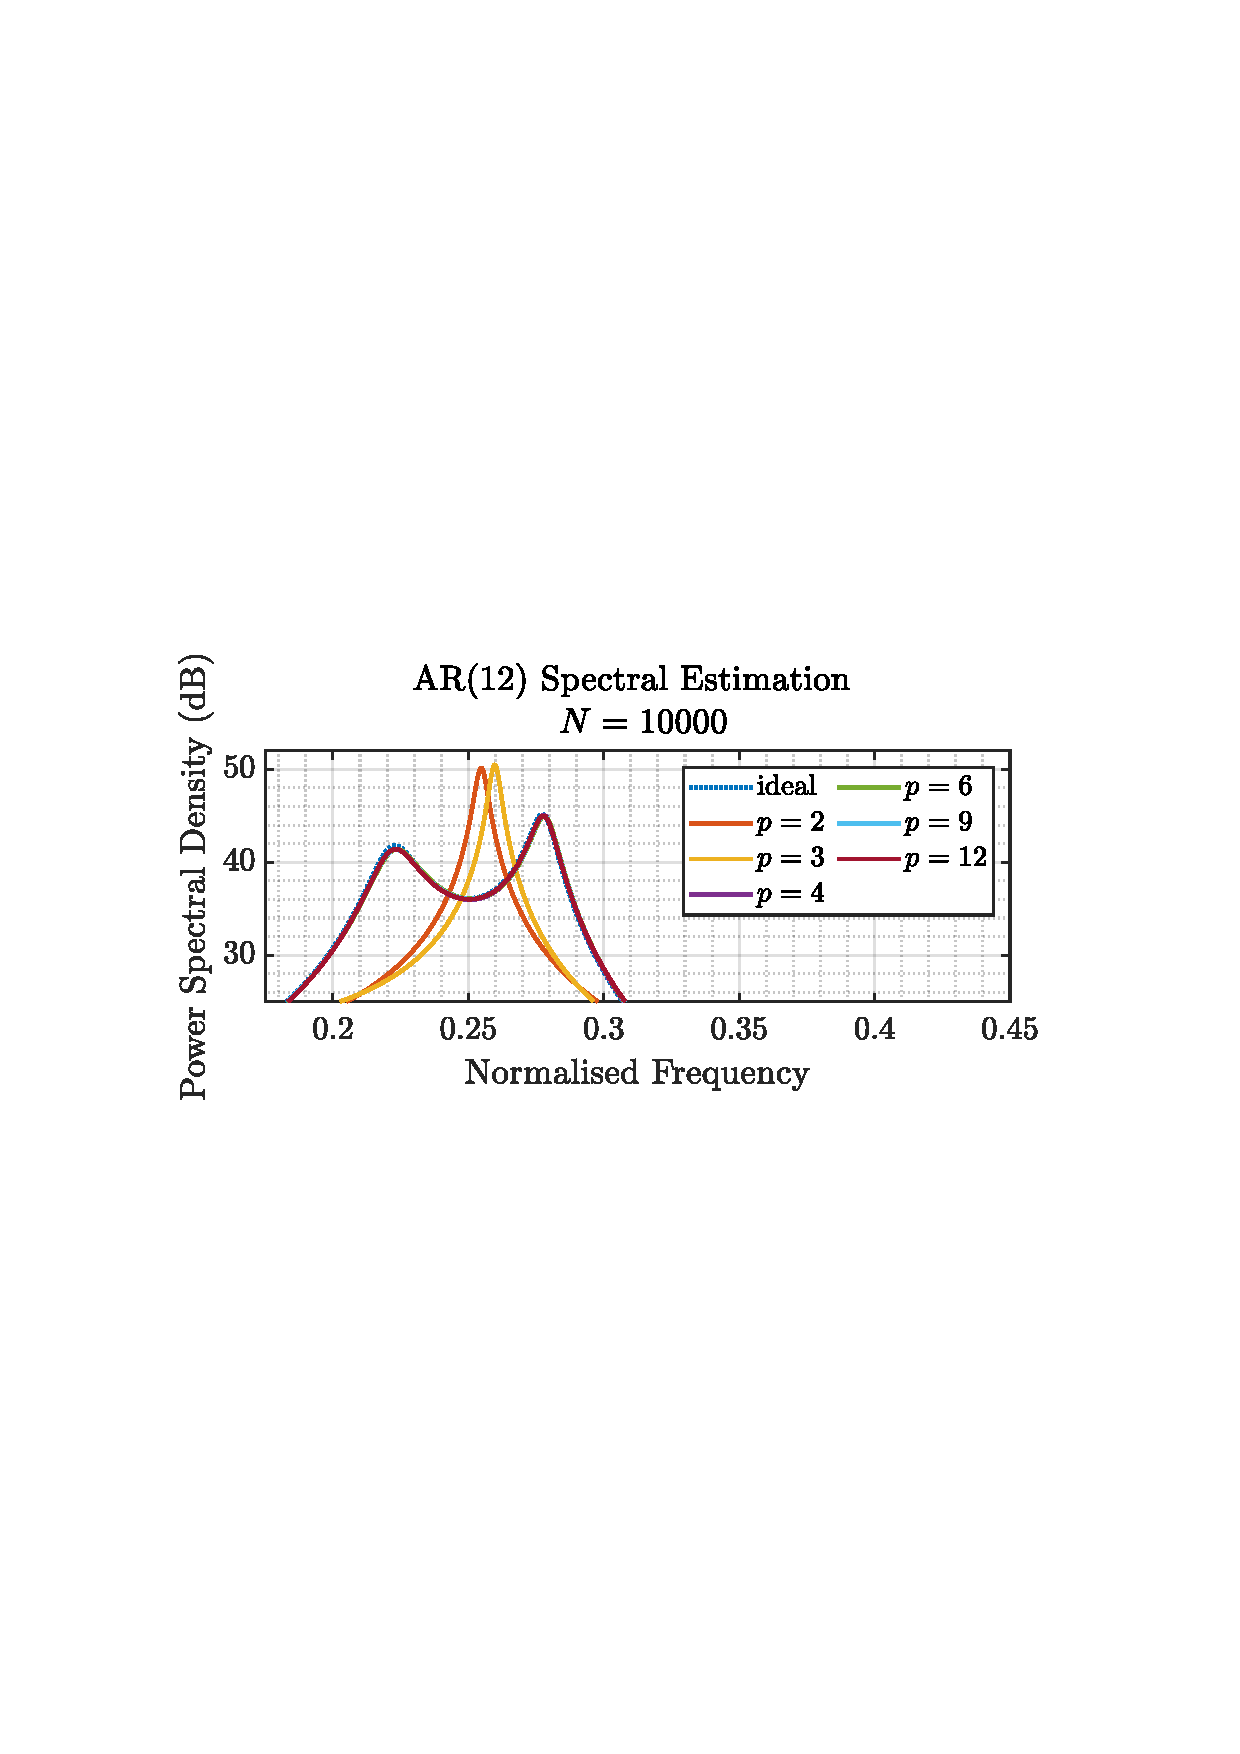
\includegraphics[trim={2.2cm 11.2cm 3.15cm  11.2cm}, clip, width=\textwidth]{../MATLAB/figures/q1_4c_fig14.pdf} 
			\captionsetup{justification=centering}
			\caption{AR Periodogram and its $p$ Order Estimates}
		\end{subfigure}
		%		~ % forces onto the same row
		\begin{subfigure}{0.49\textwidth}
			\centering
			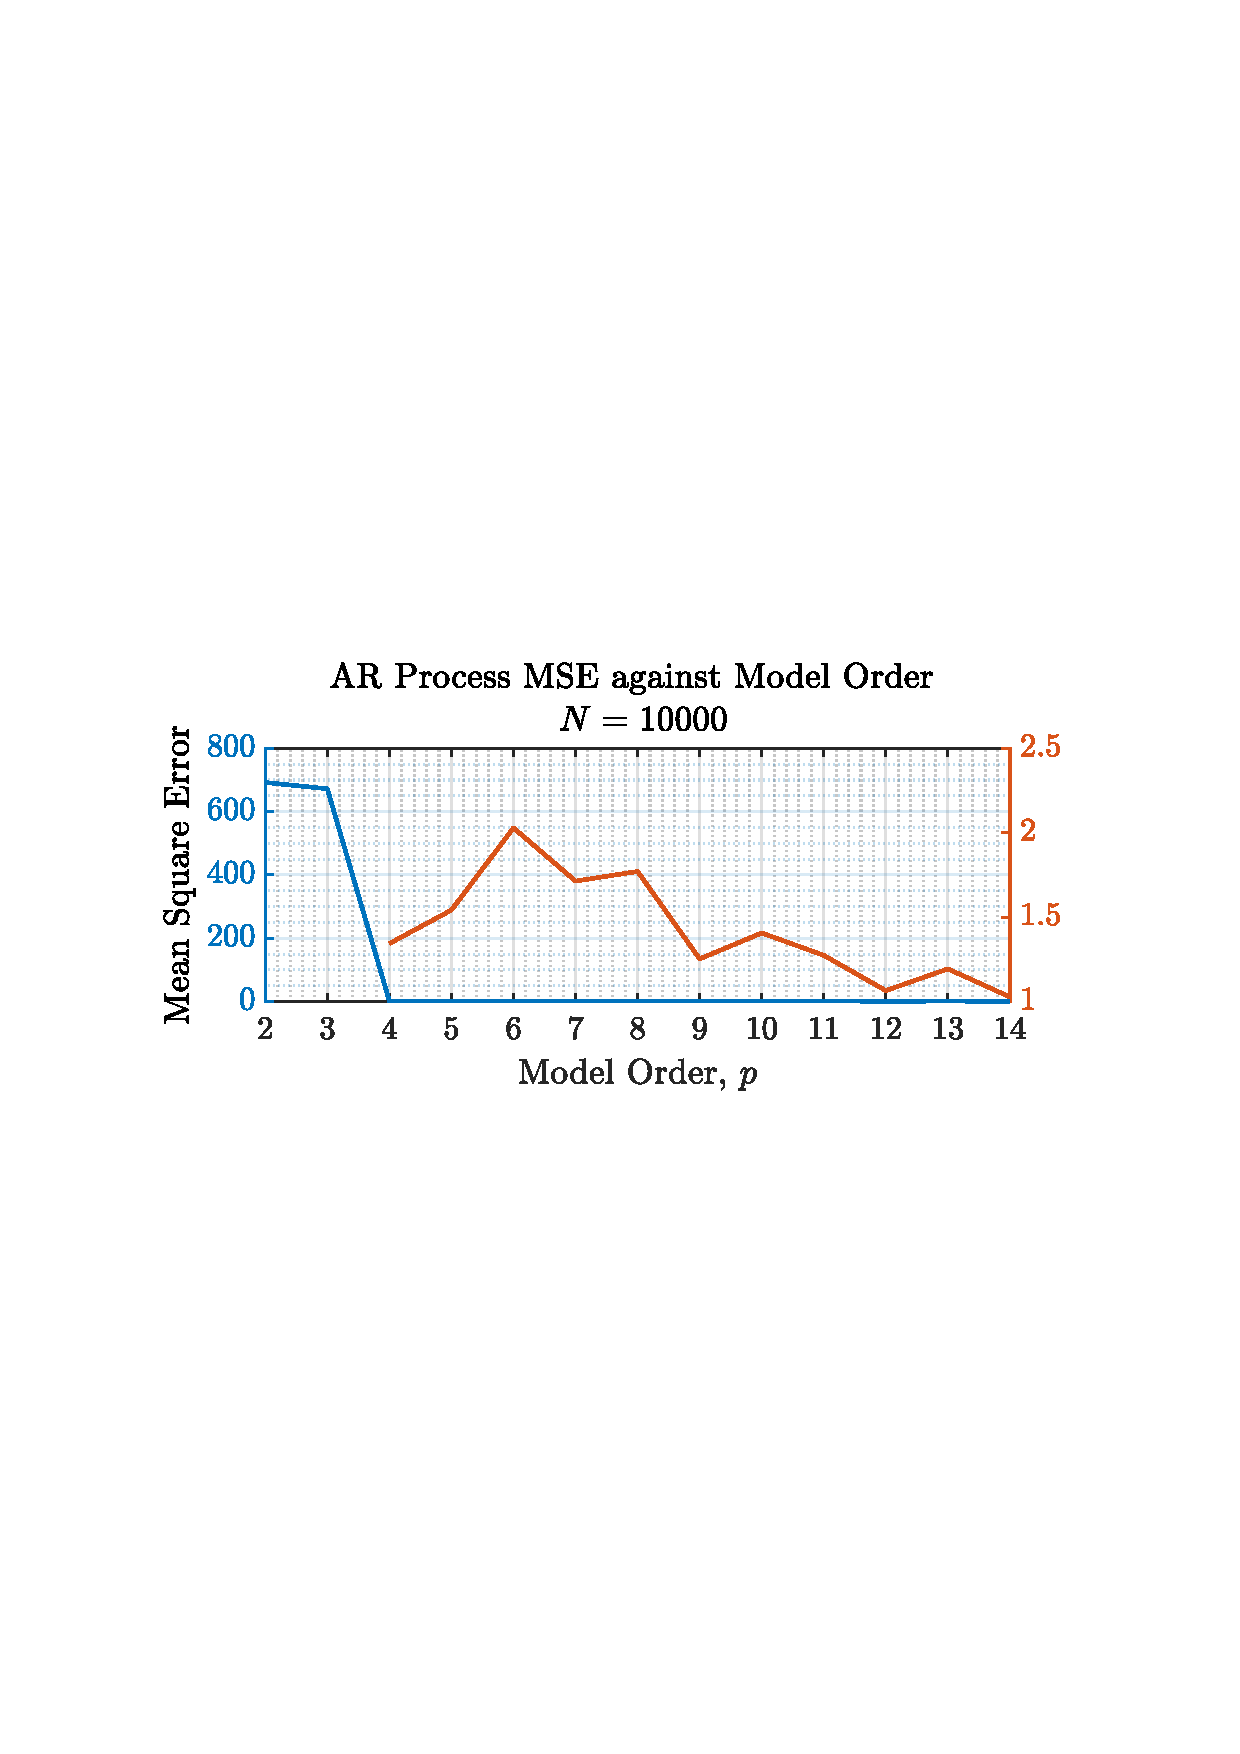
\includegraphics[trim={2.2cm 11.2cm 3.15cm  11.2cm}, clip, width=\textwidth]{../MATLAB/figures/q1_4c_fig16.pdf} 
			\captionsetup{justification=centering}
			\caption{Mean Squared Error}
		\end{subfigure}
		\label{fig: 1-4c}
	\end{figure}
	
	\subsection{Real World Signals: Respiratory Sinus Arrhythmia from RR-Intervals} \label{sec: 1-5-real-world-signals}
	% TODO: These ylabels are cut-off, definitely too long
	\subsubsection{Standard \& Average PSDs of the RRI Dataset}
	\begin{figure}[H]
		\centering
		\begin{subfigure}{0.49\textwidth}
			\centering
			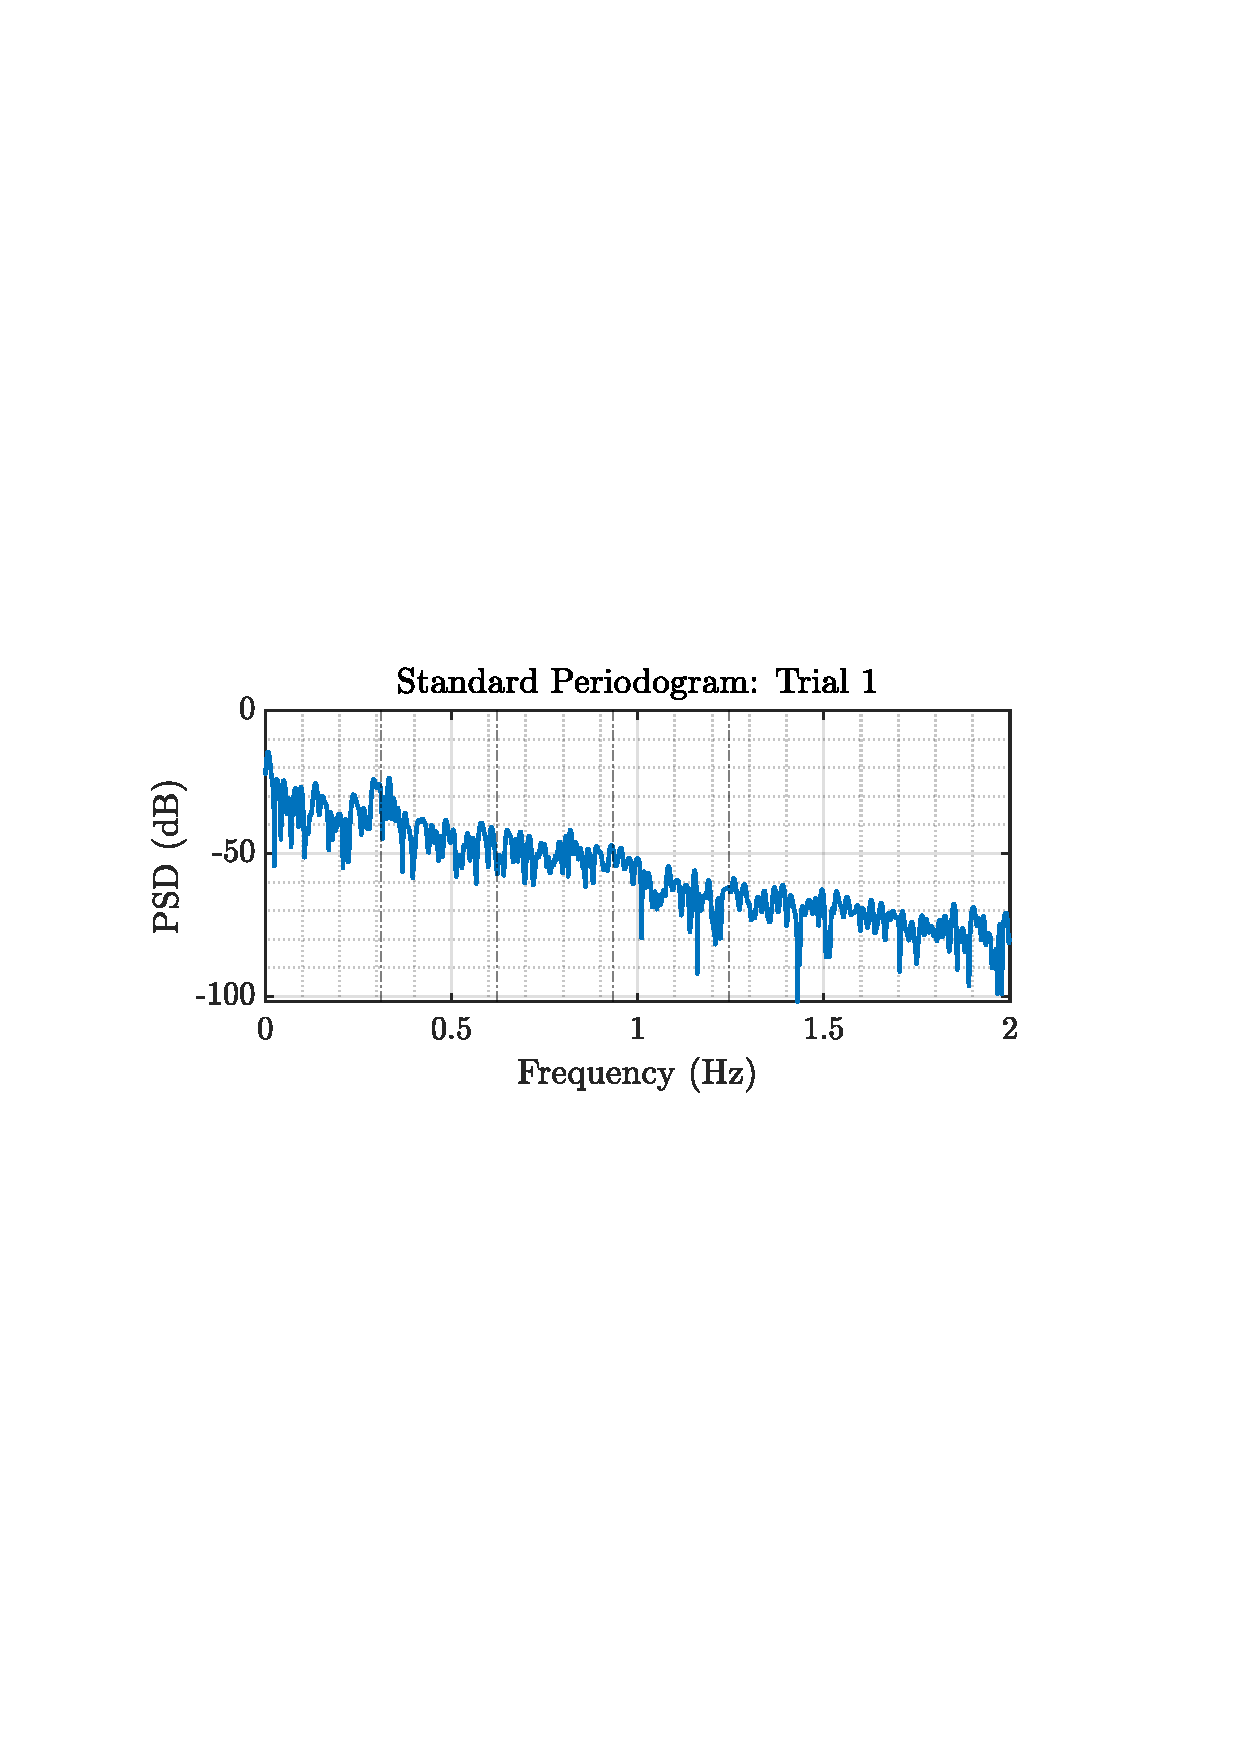
\includegraphics[trim={2.2cm 11cm 3.15cm  11.2cm}, clip, width=\textwidth]{../MATLAB/figures/q1_5a_fig01.pdf} 
		\end{subfigure}
		%		~ % forces onto the same row
		\begin{subfigure}{0.49\textwidth}
			\centering
			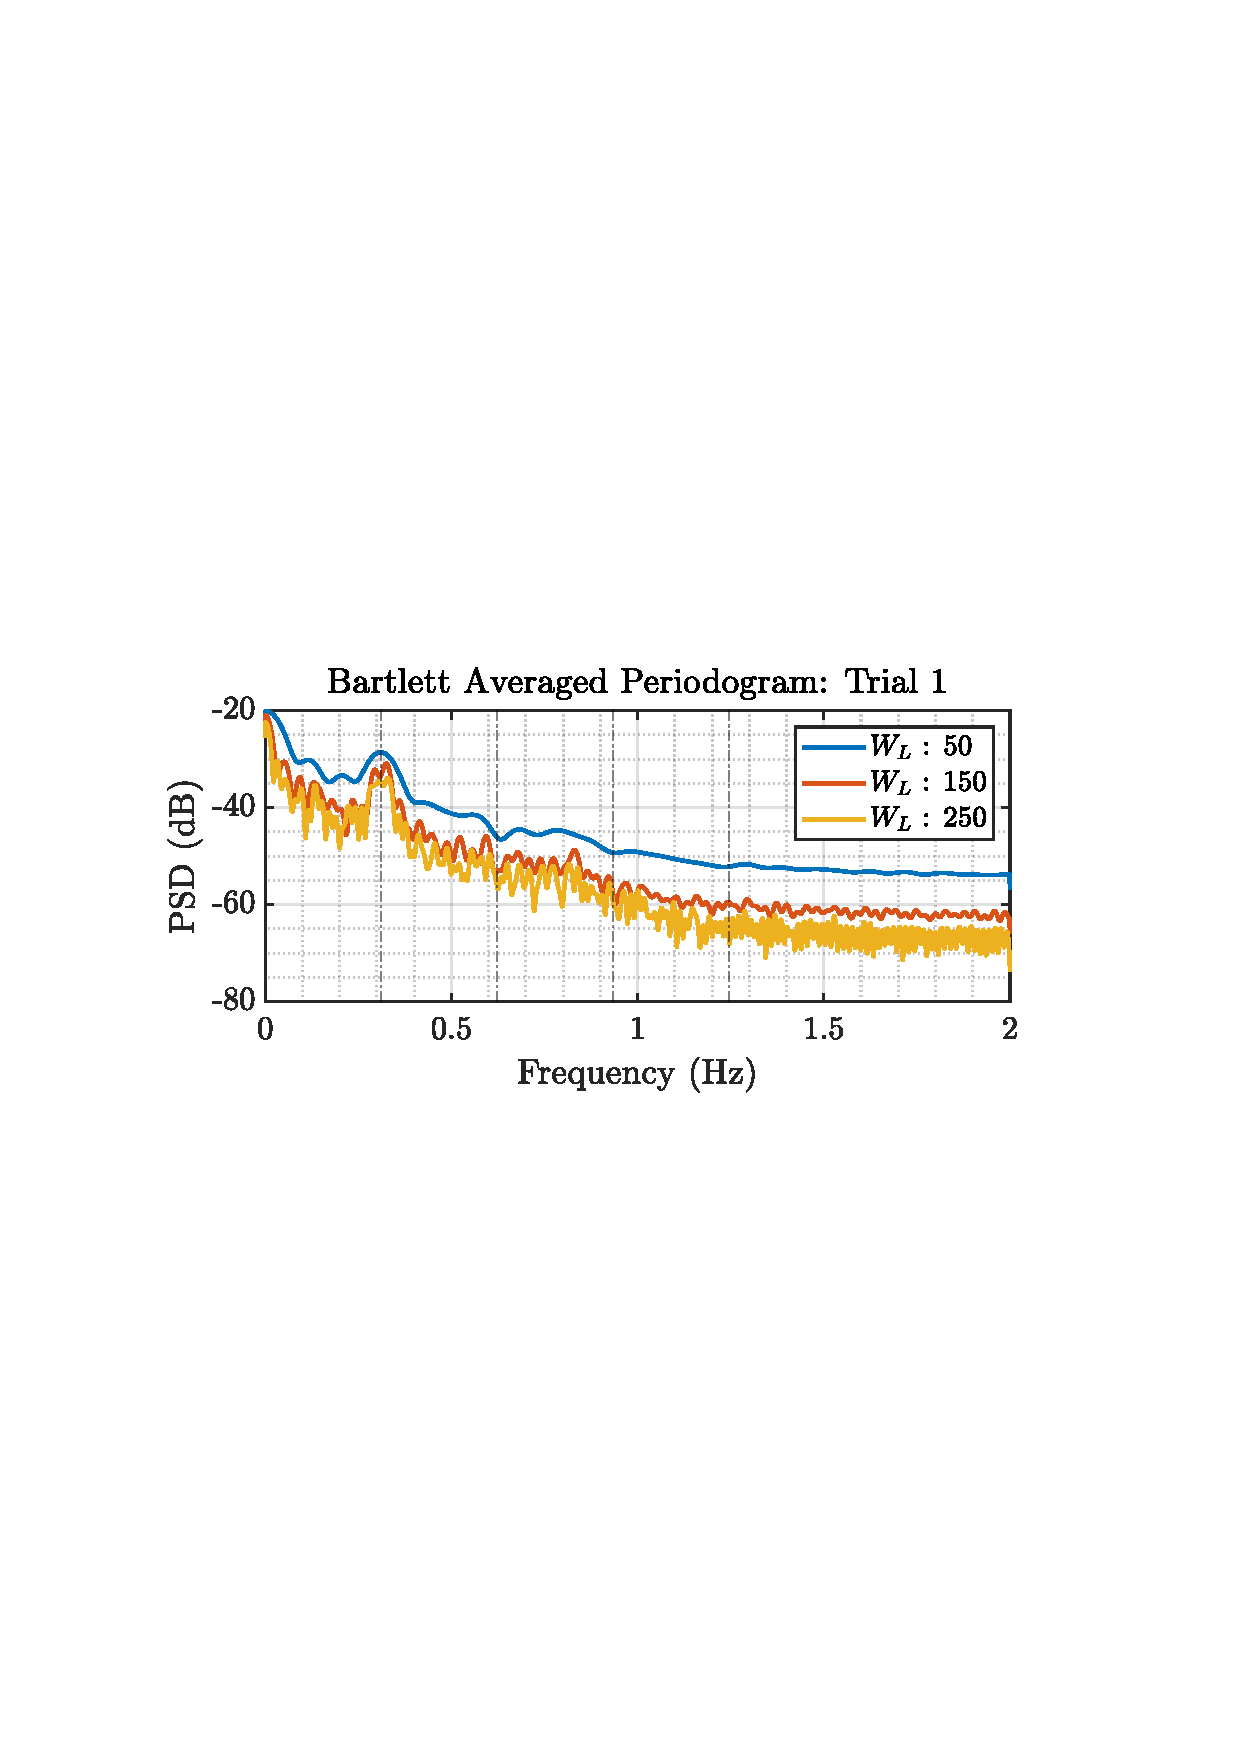
\includegraphics[trim={2.2cm 11cm 3.15cm  11.2cm}, clip, width=\textwidth]{../MATLAB/figures/q1_5a_fig04.pdf} 
		\end{subfigure}
		\begin{subfigure}{0.49\textwidth}
			\centering
			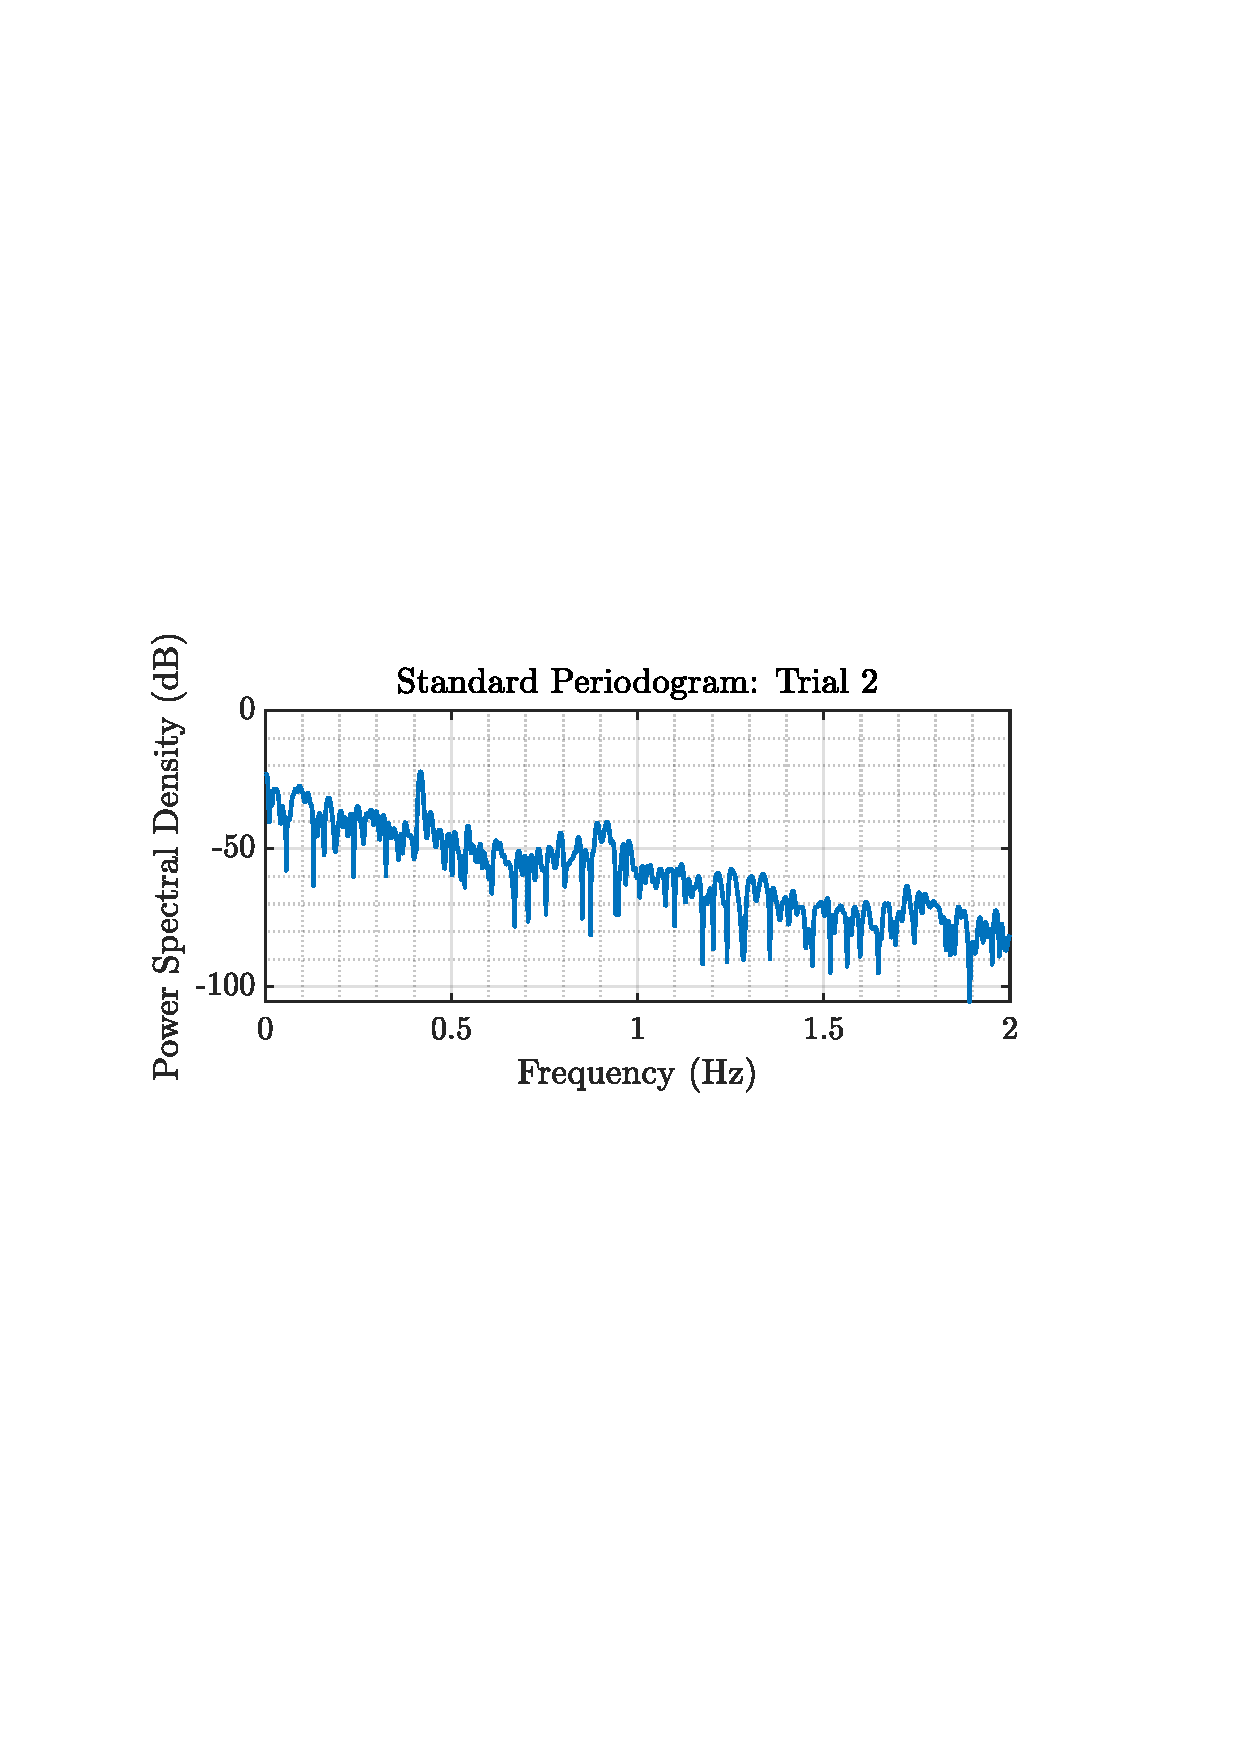
\includegraphics[trim={2.2cm 11cm 3.15cm  11.2cm}, clip, width=\textwidth]{../MATLAB/figures/q1_5a_fig02.pdf} 
		\end{subfigure}
		%		~ % forces onto the same row
		\begin{subfigure}{0.49\textwidth}
			\centering
			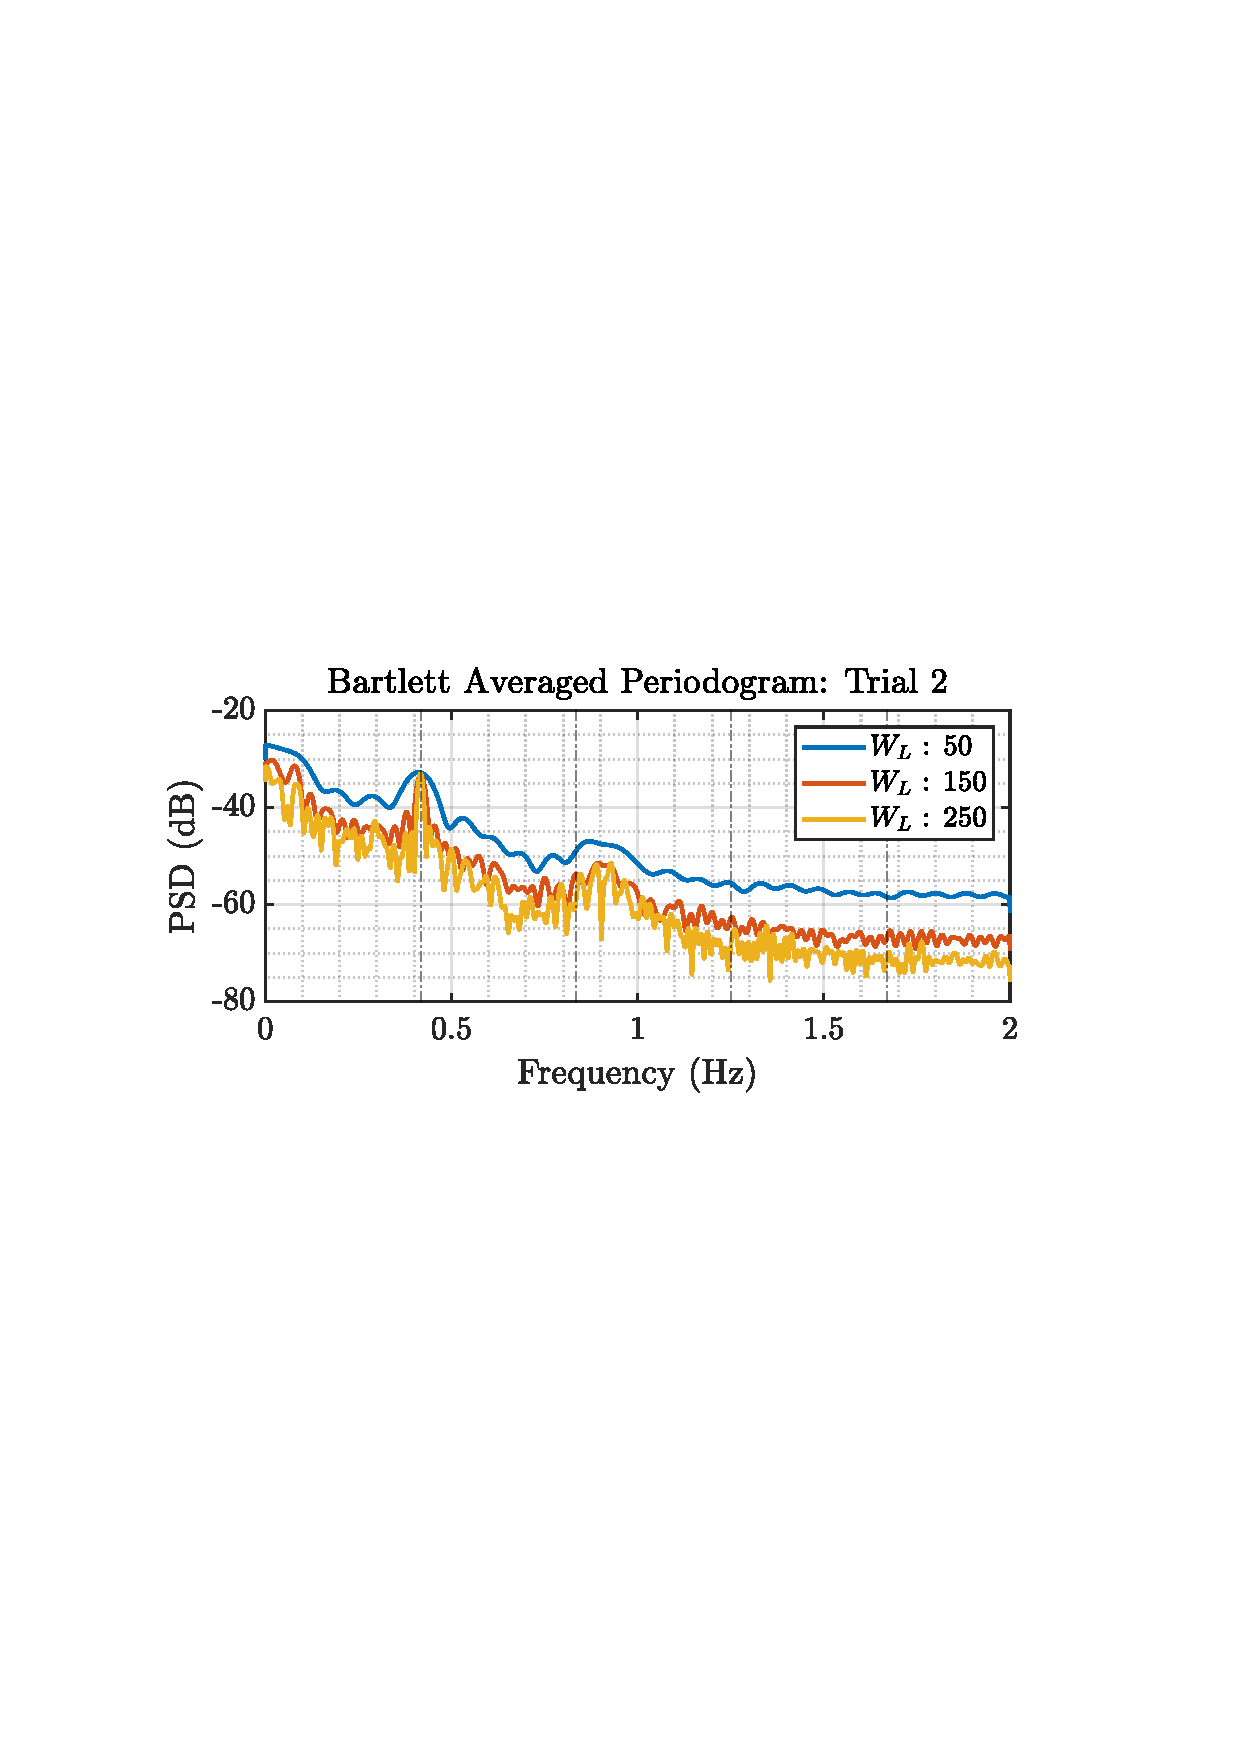
\includegraphics[trim={2.2cm 11cm 3.15cm  11.2cm}, clip, width=\textwidth]{../MATLAB/figures/q1_5a_fig05.pdf} 
		\end{subfigure}
		\begin{subfigure}{0.49\textwidth}
			\centering
			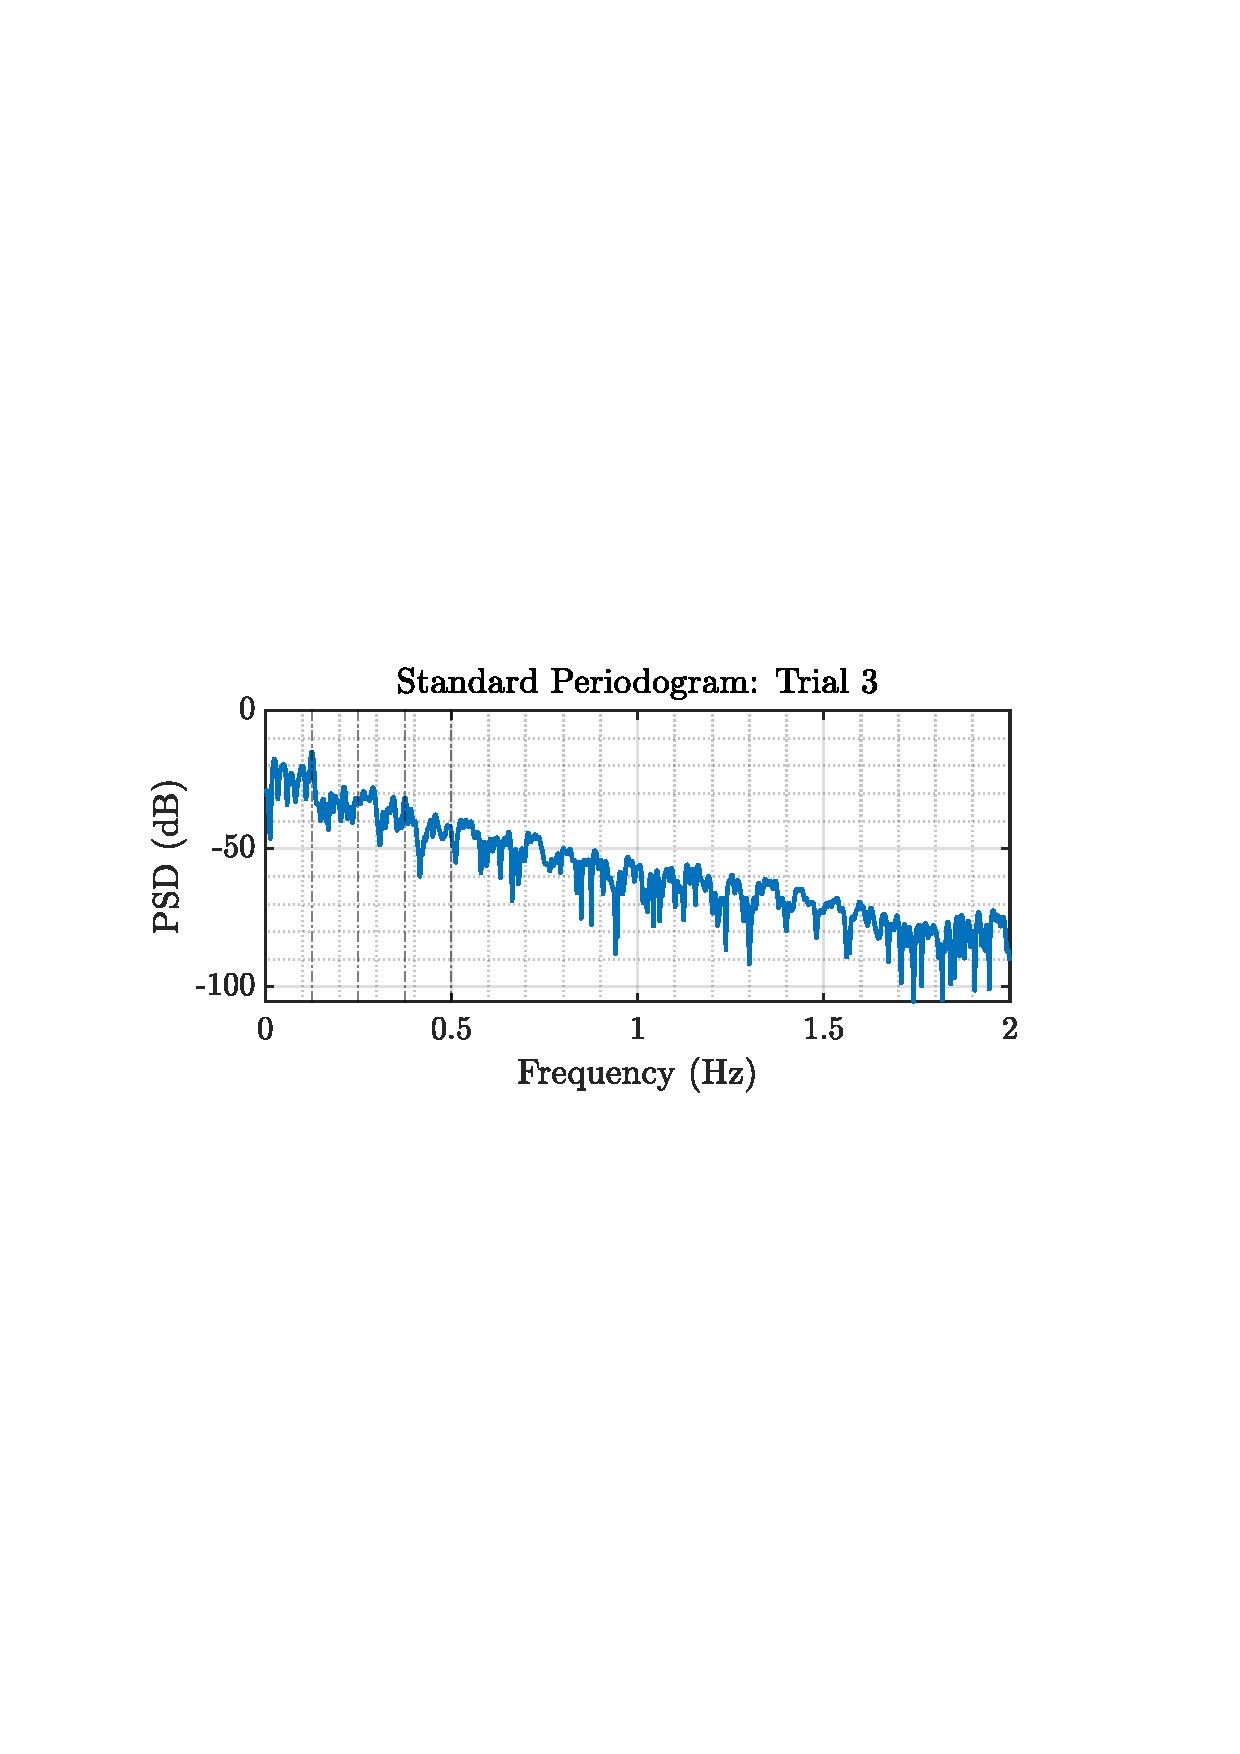
\includegraphics[trim={2.2cm 11.2cm 3.15cm  11.2cm}, clip, width=\textwidth]{../MATLAB/figures/q1_5a_fig03.pdf} 
		\end{subfigure}
		%		~ % forces onto the same row
		\begin{subfigure}{0.49\textwidth}
			\centering
			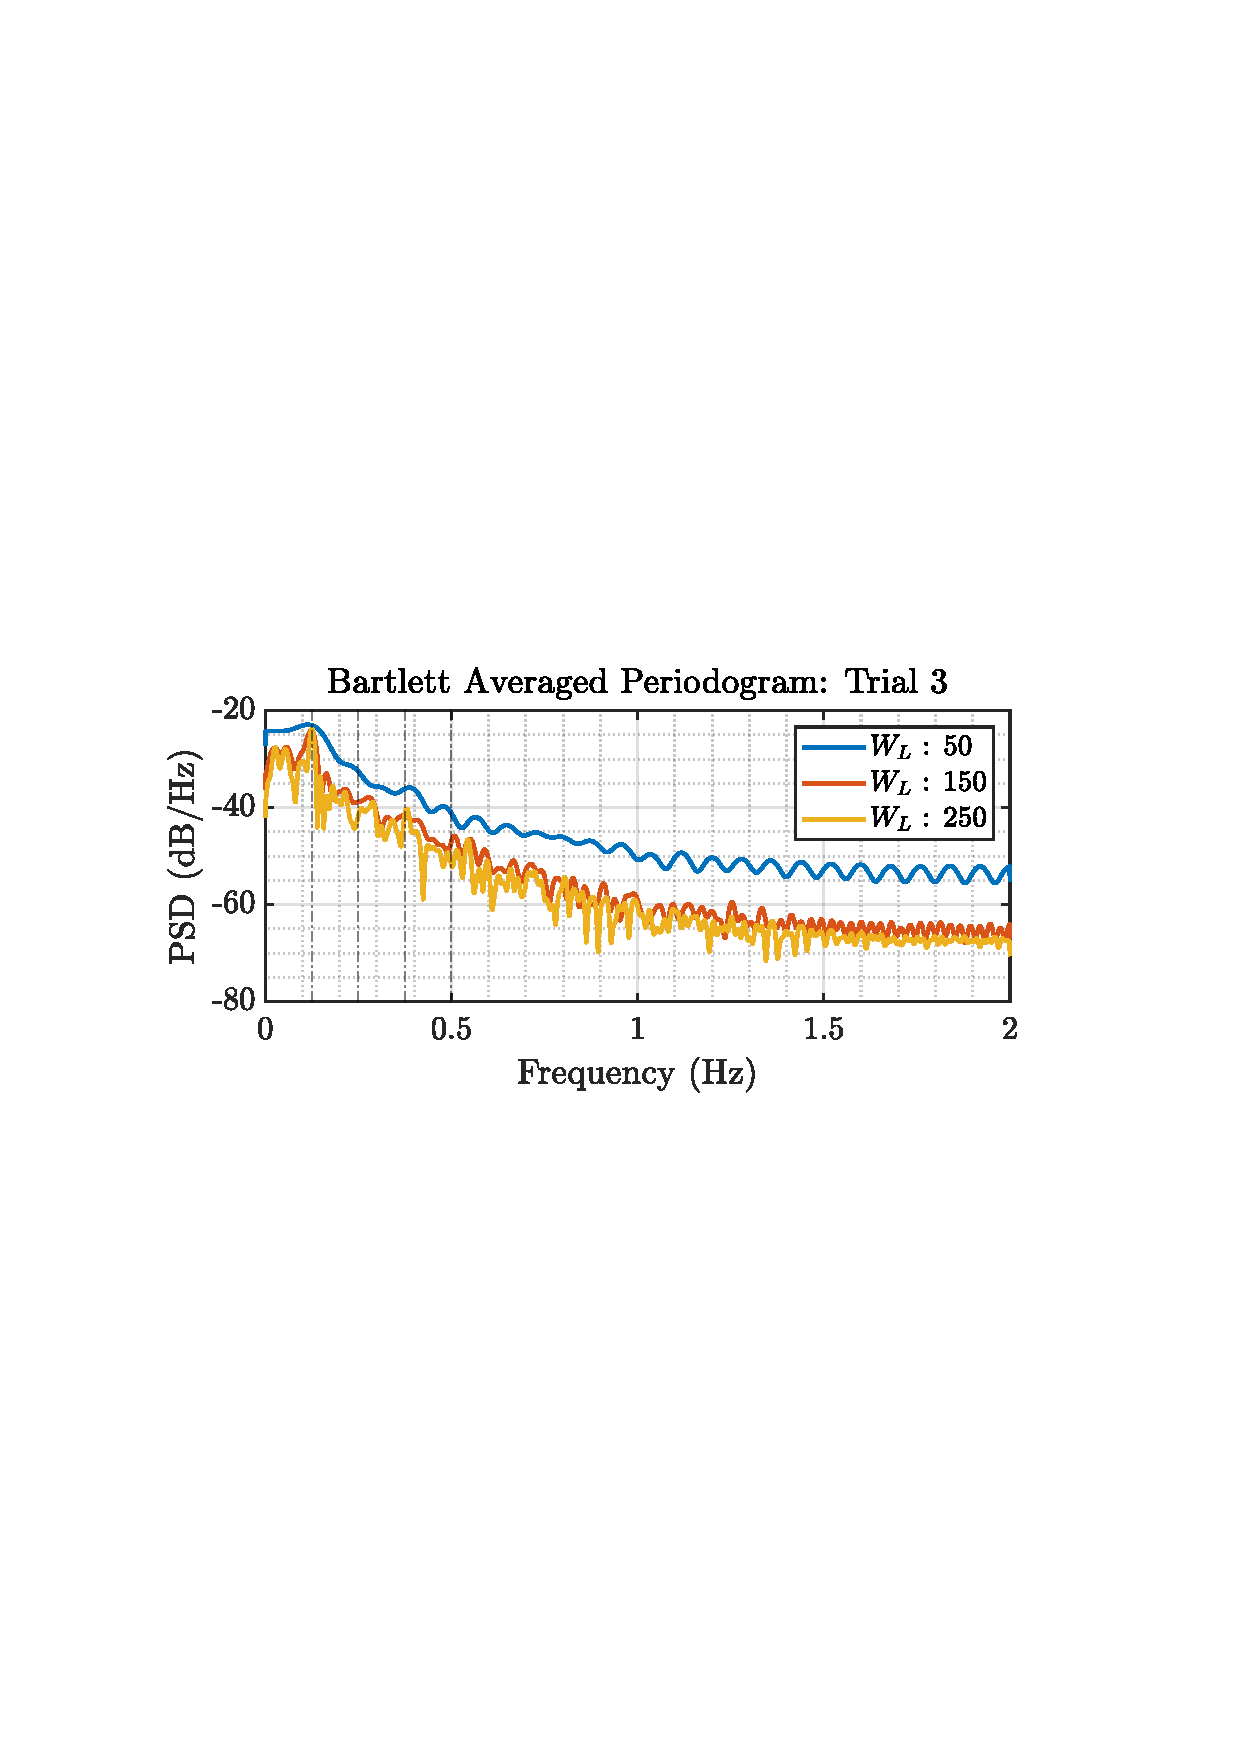
\includegraphics[trim={2.2cm 11.2cm 3.15cm  11.2cm}, clip, width=\textwidth]{../MATLAB/figures/q1_5a_fig06.pdf} 
		\end{subfigure}
		\captionsetup{justification=centering}
		\caption{Standard and Bartlett Average Periodograms. \\ $W_L$ is the Window Length used}
		\label{fig: 1-5a}
	\end{figure}

	\subsubsection{Analysis of the RRI PSD Estimates}
	
	\subsubsection{AR PSD Estimate for the RRI Dataset}
	Test text \\
	\begin{wrapfigure}{r}{0.49\textwidth}
		\vspace{-20pt}
		\begin{centering}
			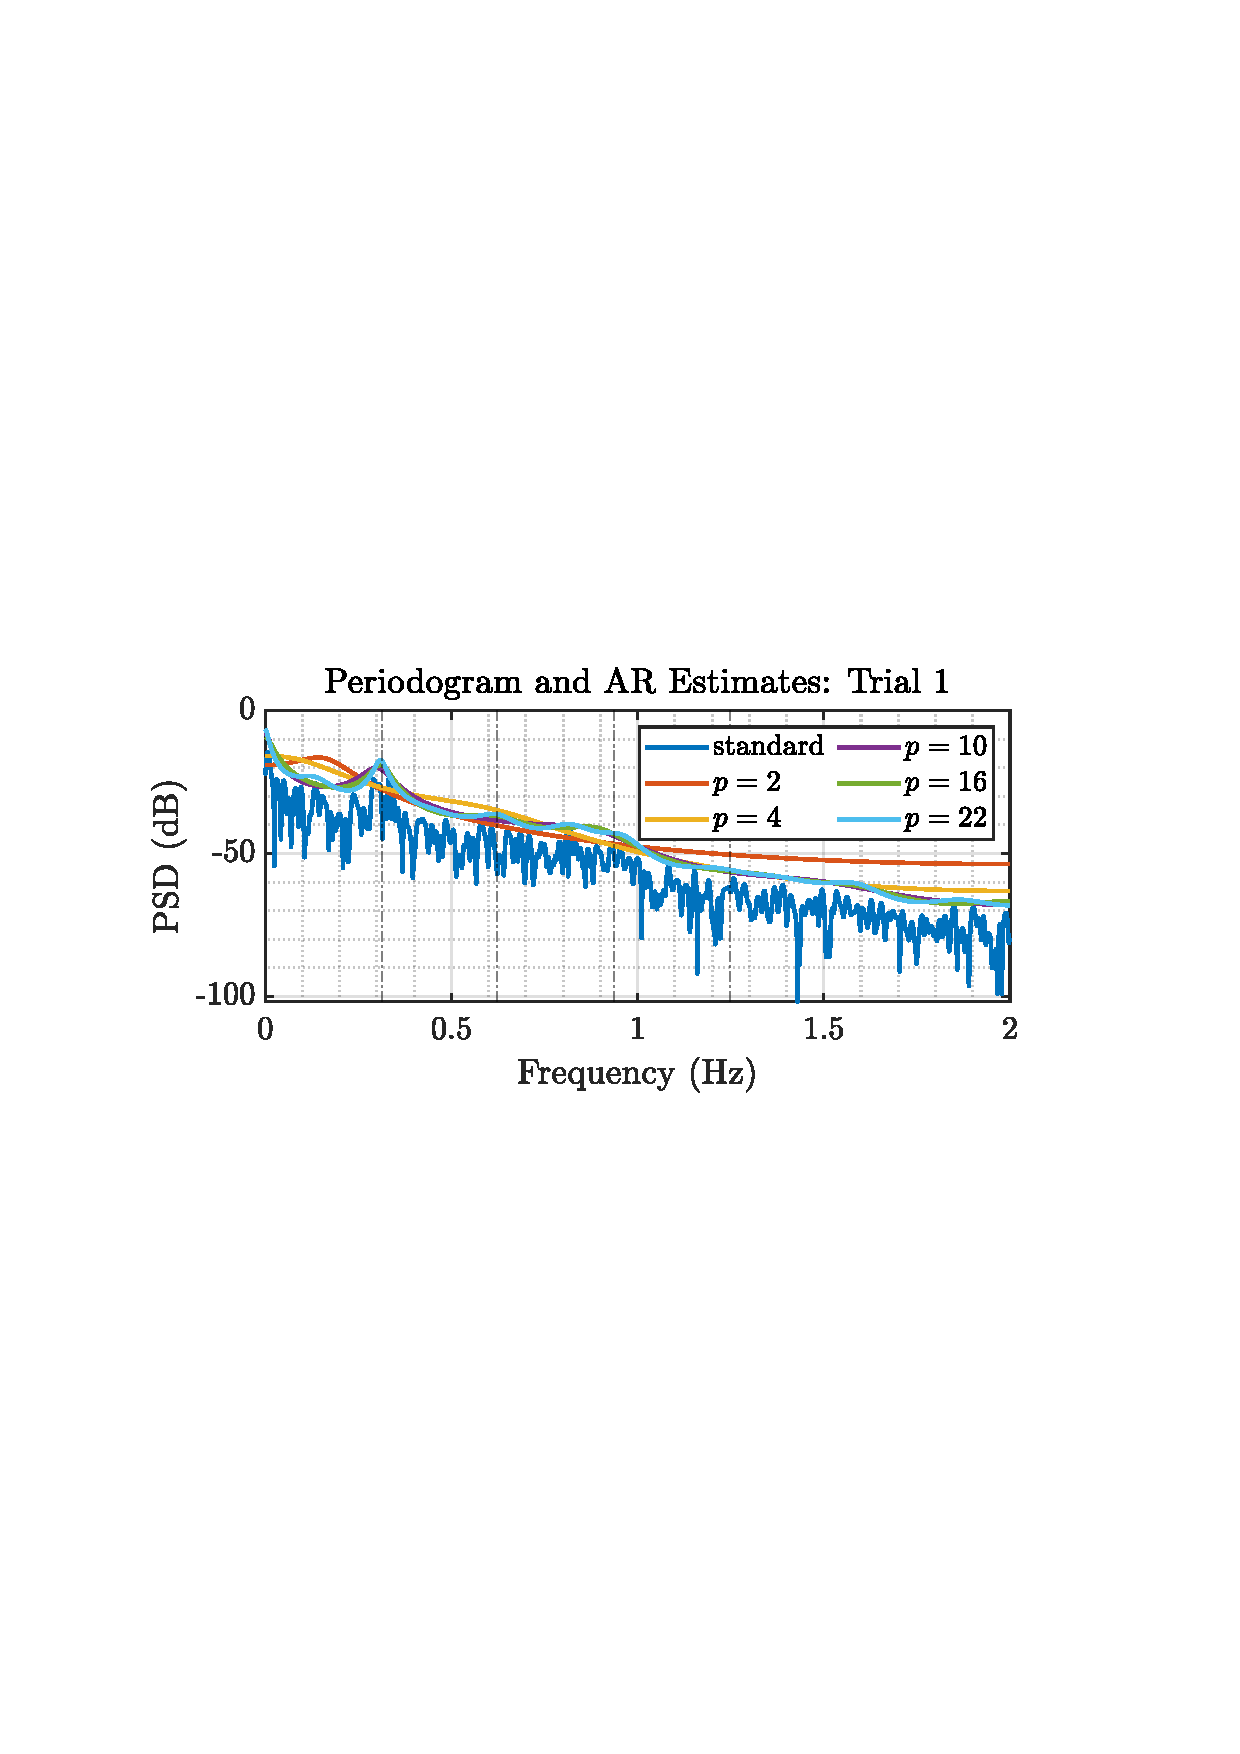
\includegraphics[trim={2.2cm 11.2cm 3.15cm  11.2cm}, clip, width=0.49\textwidth]{../MATLAB/figures/q1_5c_fig01.pdf} 
		\end{centering}
%		\vspace{-20pt}
%		\vspace{-10pt}
		\begin{centering}
			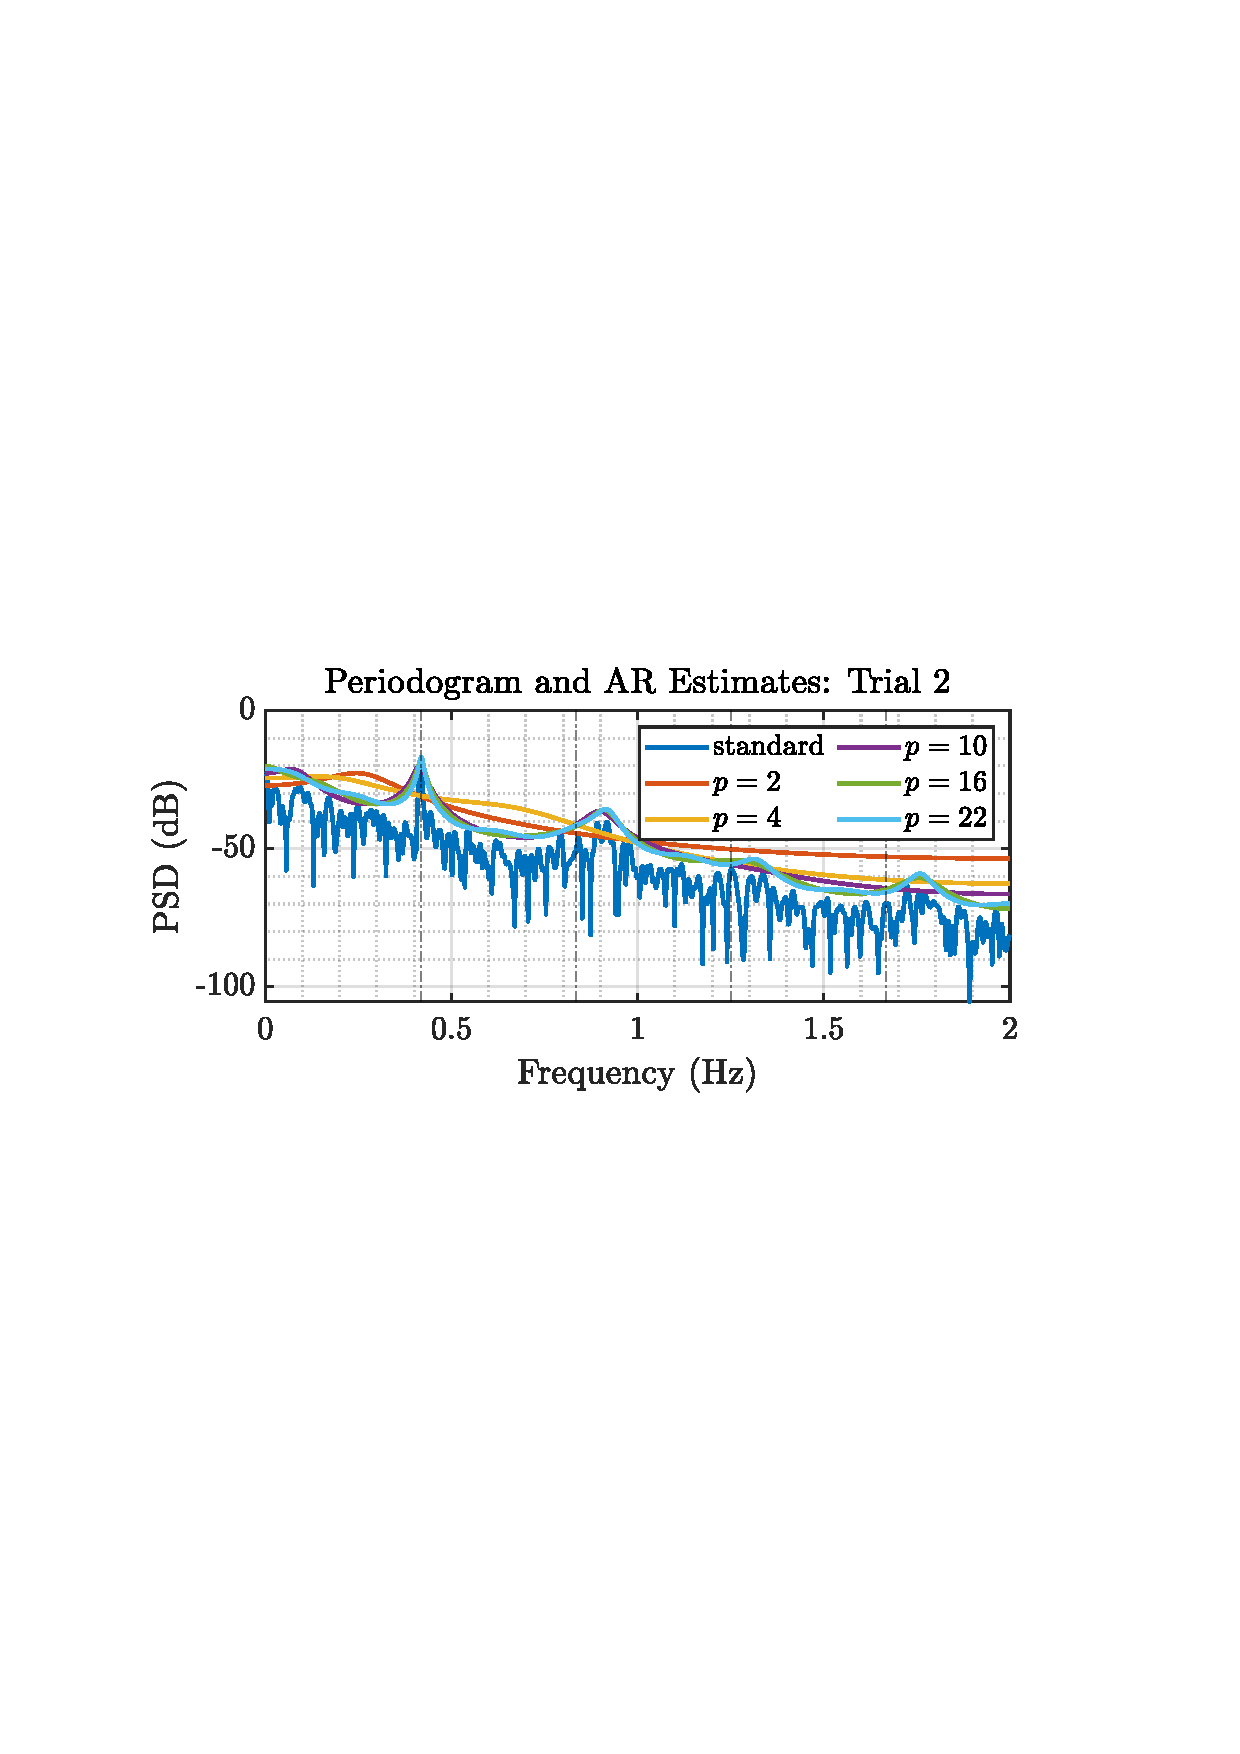
\includegraphics[trim={2.2cm 11.2cm 3.15cm  11.2cm}, clip, width=0.49\textwidth]{../MATLAB/figures/q1_5c_fig02.pdf} 
		\end{centering}
%		\vspace{-20pt}
%		\vspace{-10pt}
		\begin{centering}
			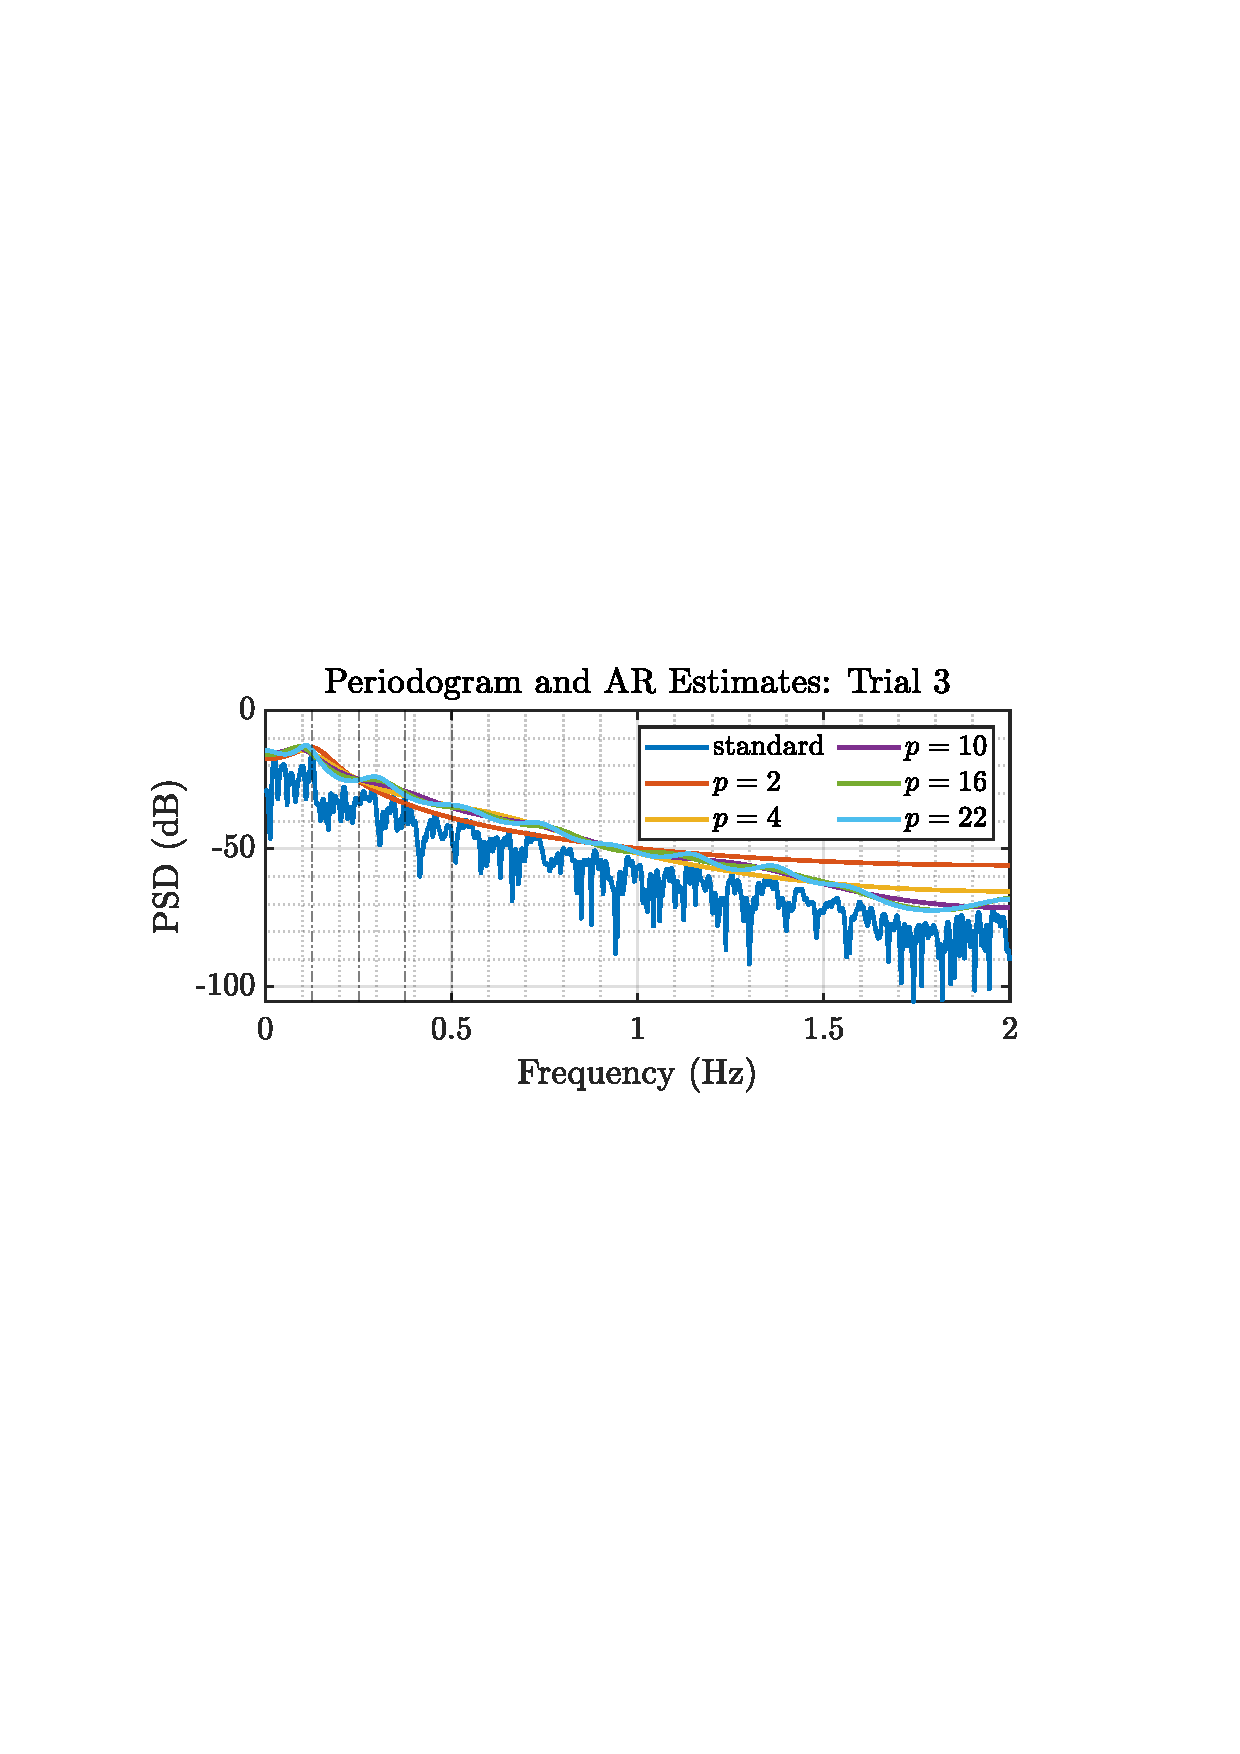
\includegraphics[trim={2.2cm 11.2cm 3.15cm  11.2cm}, clip, width=0.49\textwidth]{../MATLAB/figures/q1_5c_fig03.pdf} 
		\end{centering}
%		\vspace{-20pt}
		\captionsetup{justification=centering}
		\caption{AR Estimate Periodograms. \\ $p$ is the model order.}
%		\vspace{-10pt}
	\end{wrapfigure}
	
	\pagebreak
	
	\subsection{Robust Regression} \label{sec: 1-6-robust-regression}
 
 	\subsubsection{Single Value Decomposition (SVD)}
	\begin{figure}[H]
		\centering
		\begin{subfigure}{0.49\textwidth}
			\centering
			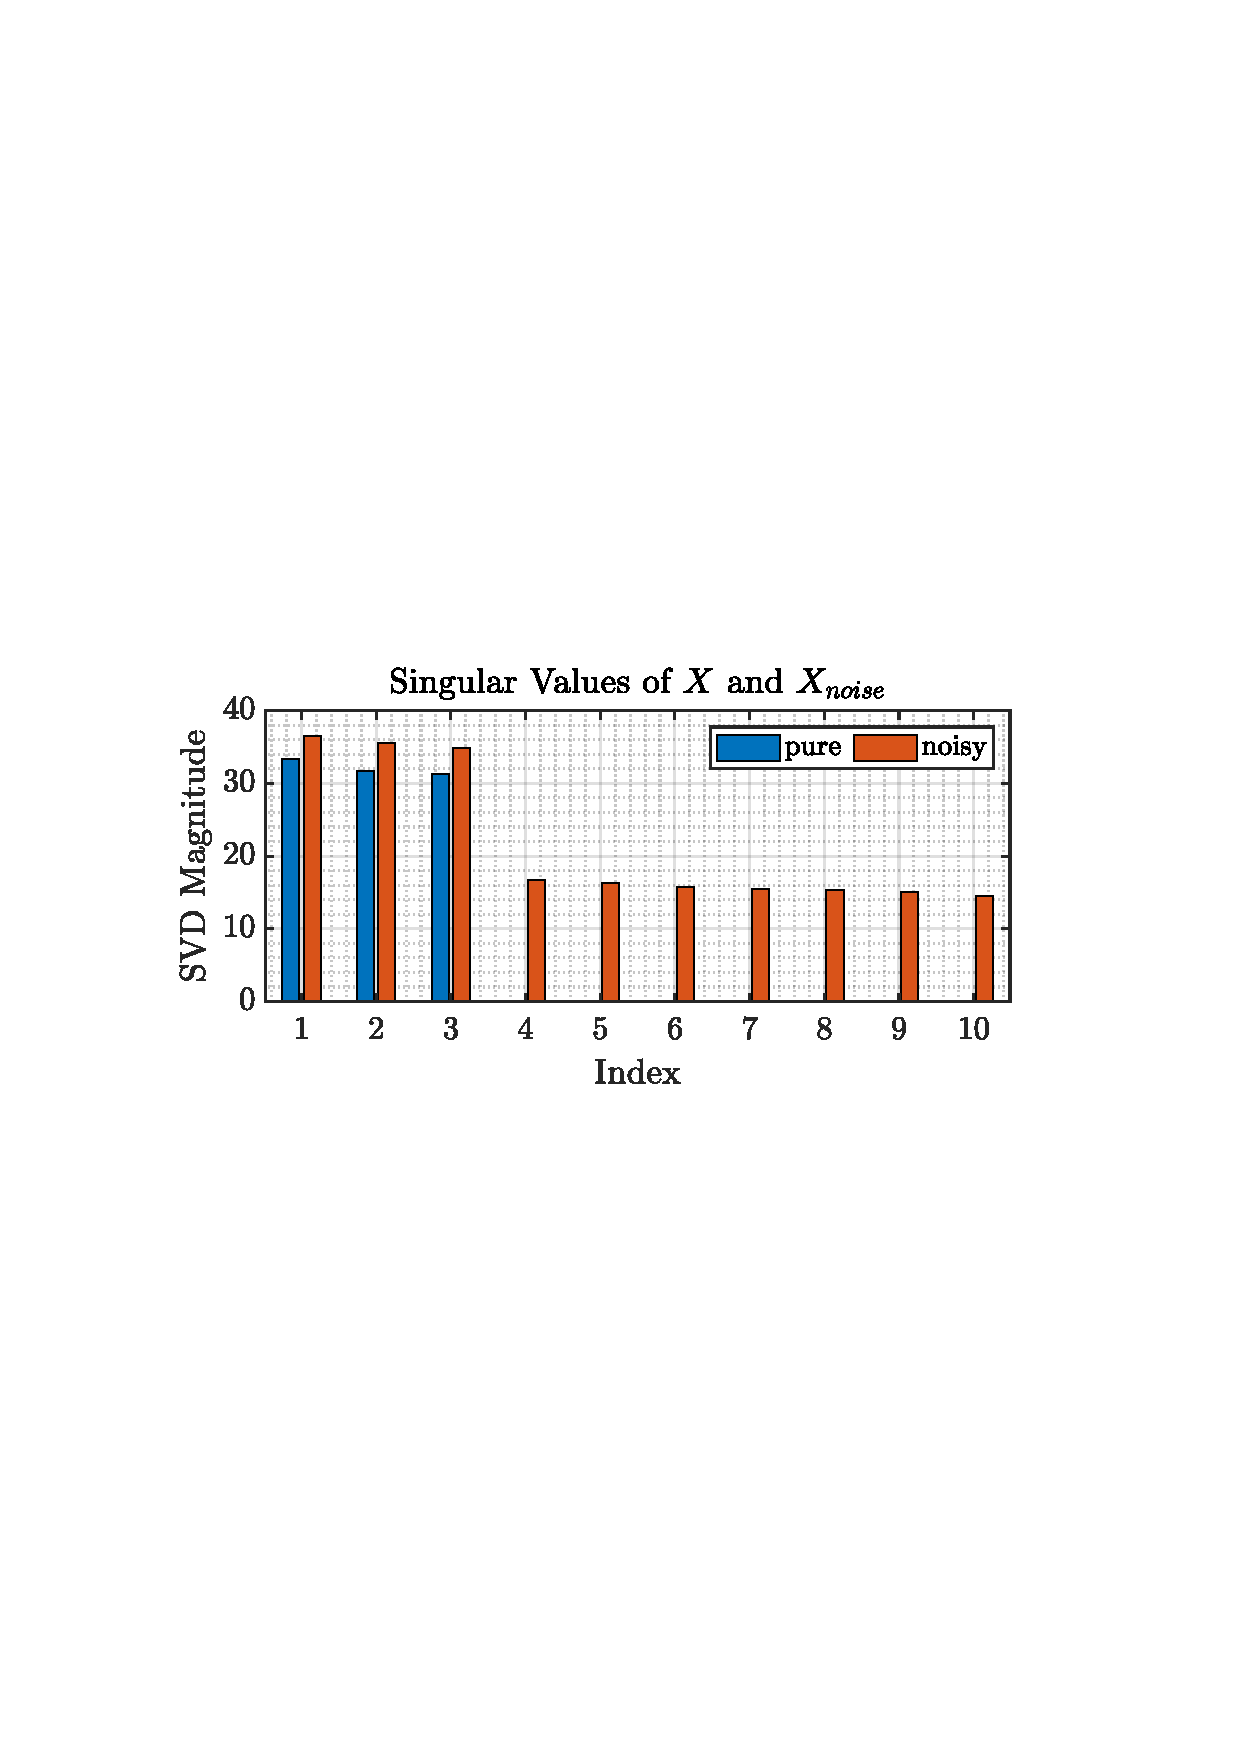
\includegraphics[trim={2.2cm 11.2cm 3.15cm  11.2cm}, clip, width=\textwidth]{../MATLAB/figures/q1_6a_fig01.pdf} 
			\captionsetup{justification=centering}
			\caption{SVD}
		\end{subfigure}
		%		~ % forces onto the same row
		\begin{subfigure}{0.49\textwidth}
			\centering
			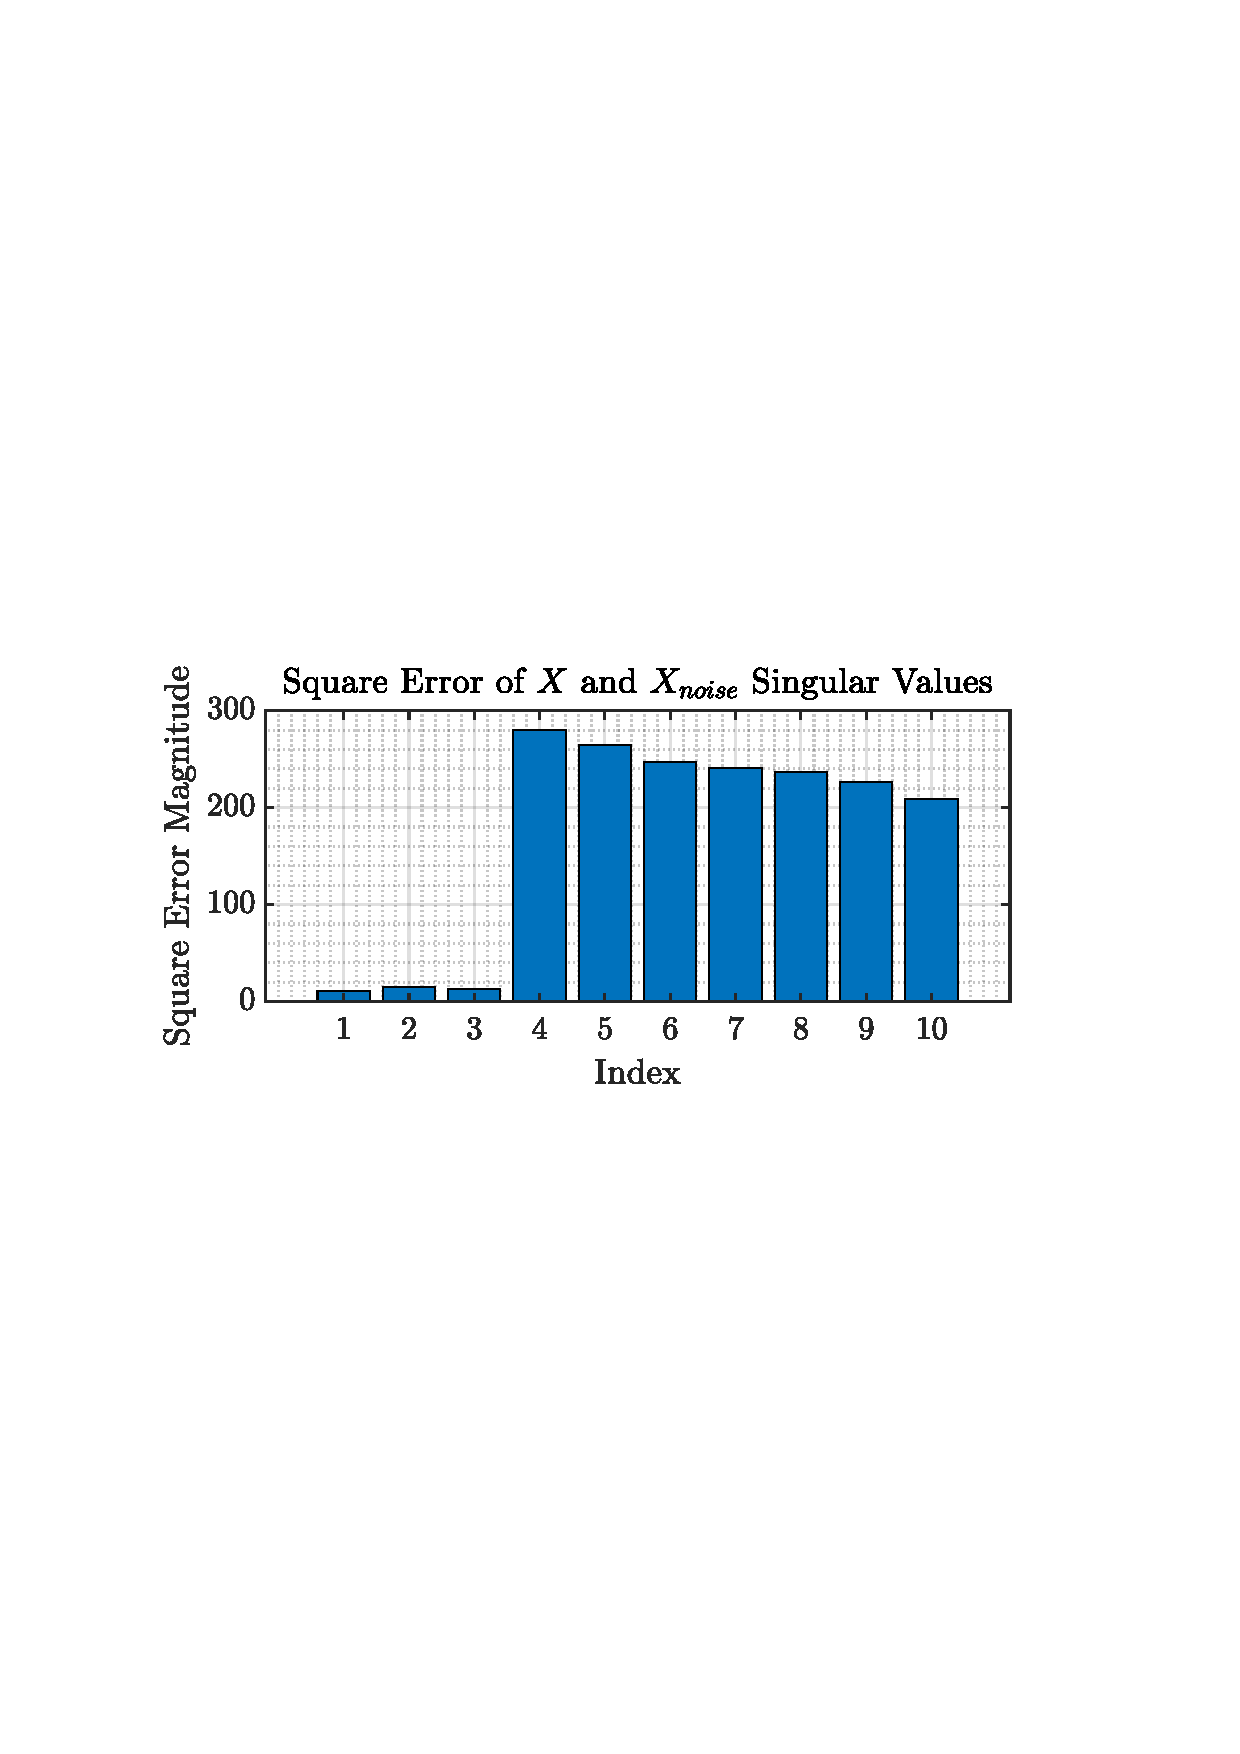
\includegraphics[trim={2.2cm 11.2cm 3.15cm  11.2cm}, clip, width=\textwidth]{../MATLAB/figures/q1_6a_fig02.pdf} 
			\captionsetup{justification=centering}
			\caption{Square Error}
		\end{subfigure}
		\label{fig: 1-6a}
	\end{figure}
 
 	\subsubsection{Low Rank Approximation Error}
 	 \begin{figure}[H]
 		\centering
 		\begin{subfigure}{0.49\textwidth}
 			\centering
 			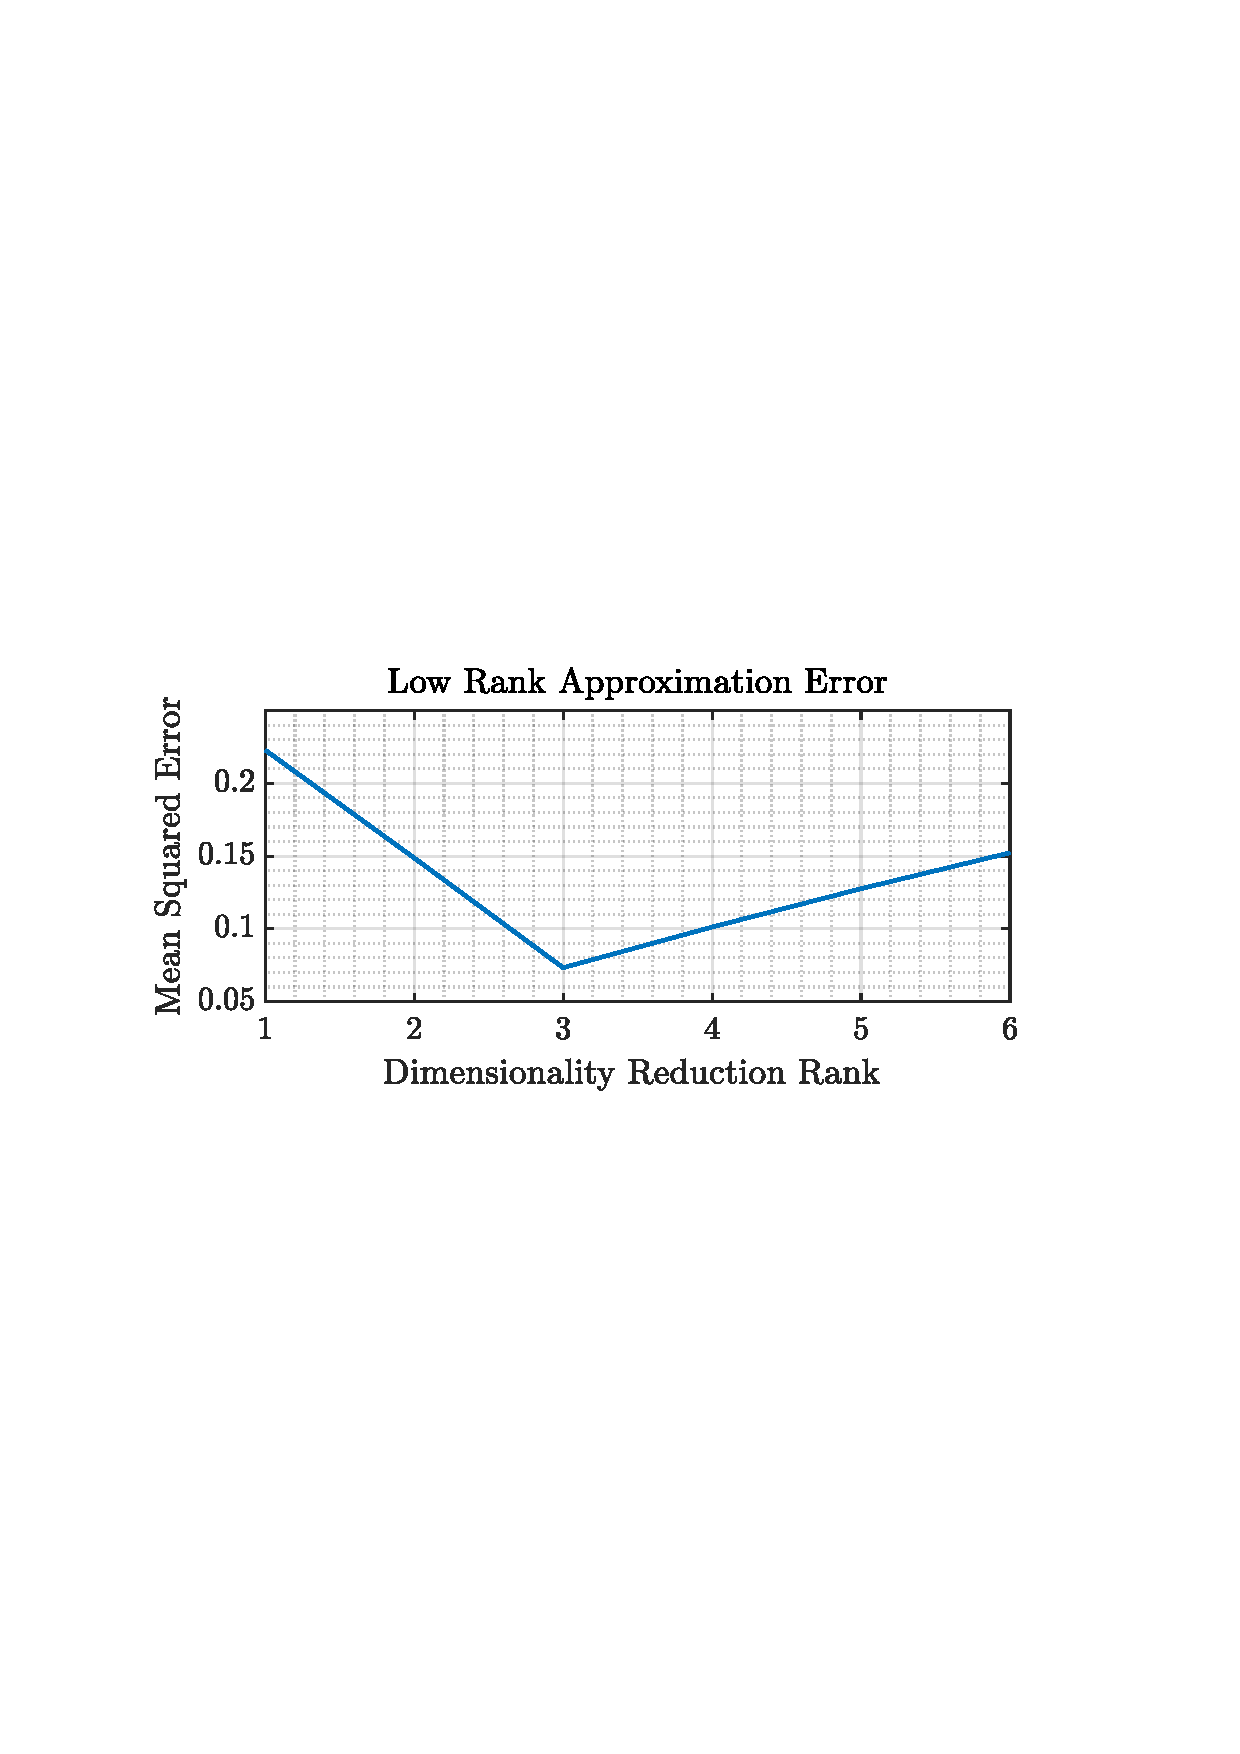
\includegraphics[trim={2.2cm 11.2cm 3.15cm  11.2cm}, clip, width=\textwidth]{../MATLAB/figures/q1_6b_fig01.pdf} 
 			\captionsetup{justification=centering}
 			\caption{Effect of Lower Ranks on the Approximation Error}
 		\end{subfigure}
 		%		~ % forces onto the same row
 		\label{fig: 1-6b}
 	\end{figure}

 	
 	\subsubsection{Ordinary Least Squares (OLS) \& Principle Component Regression (PCR)  Estimate Errors}
 	\begin{figure}[H]
 		\centering
 		\begin{subfigure}{0.49\textwidth}
 			\centering
 			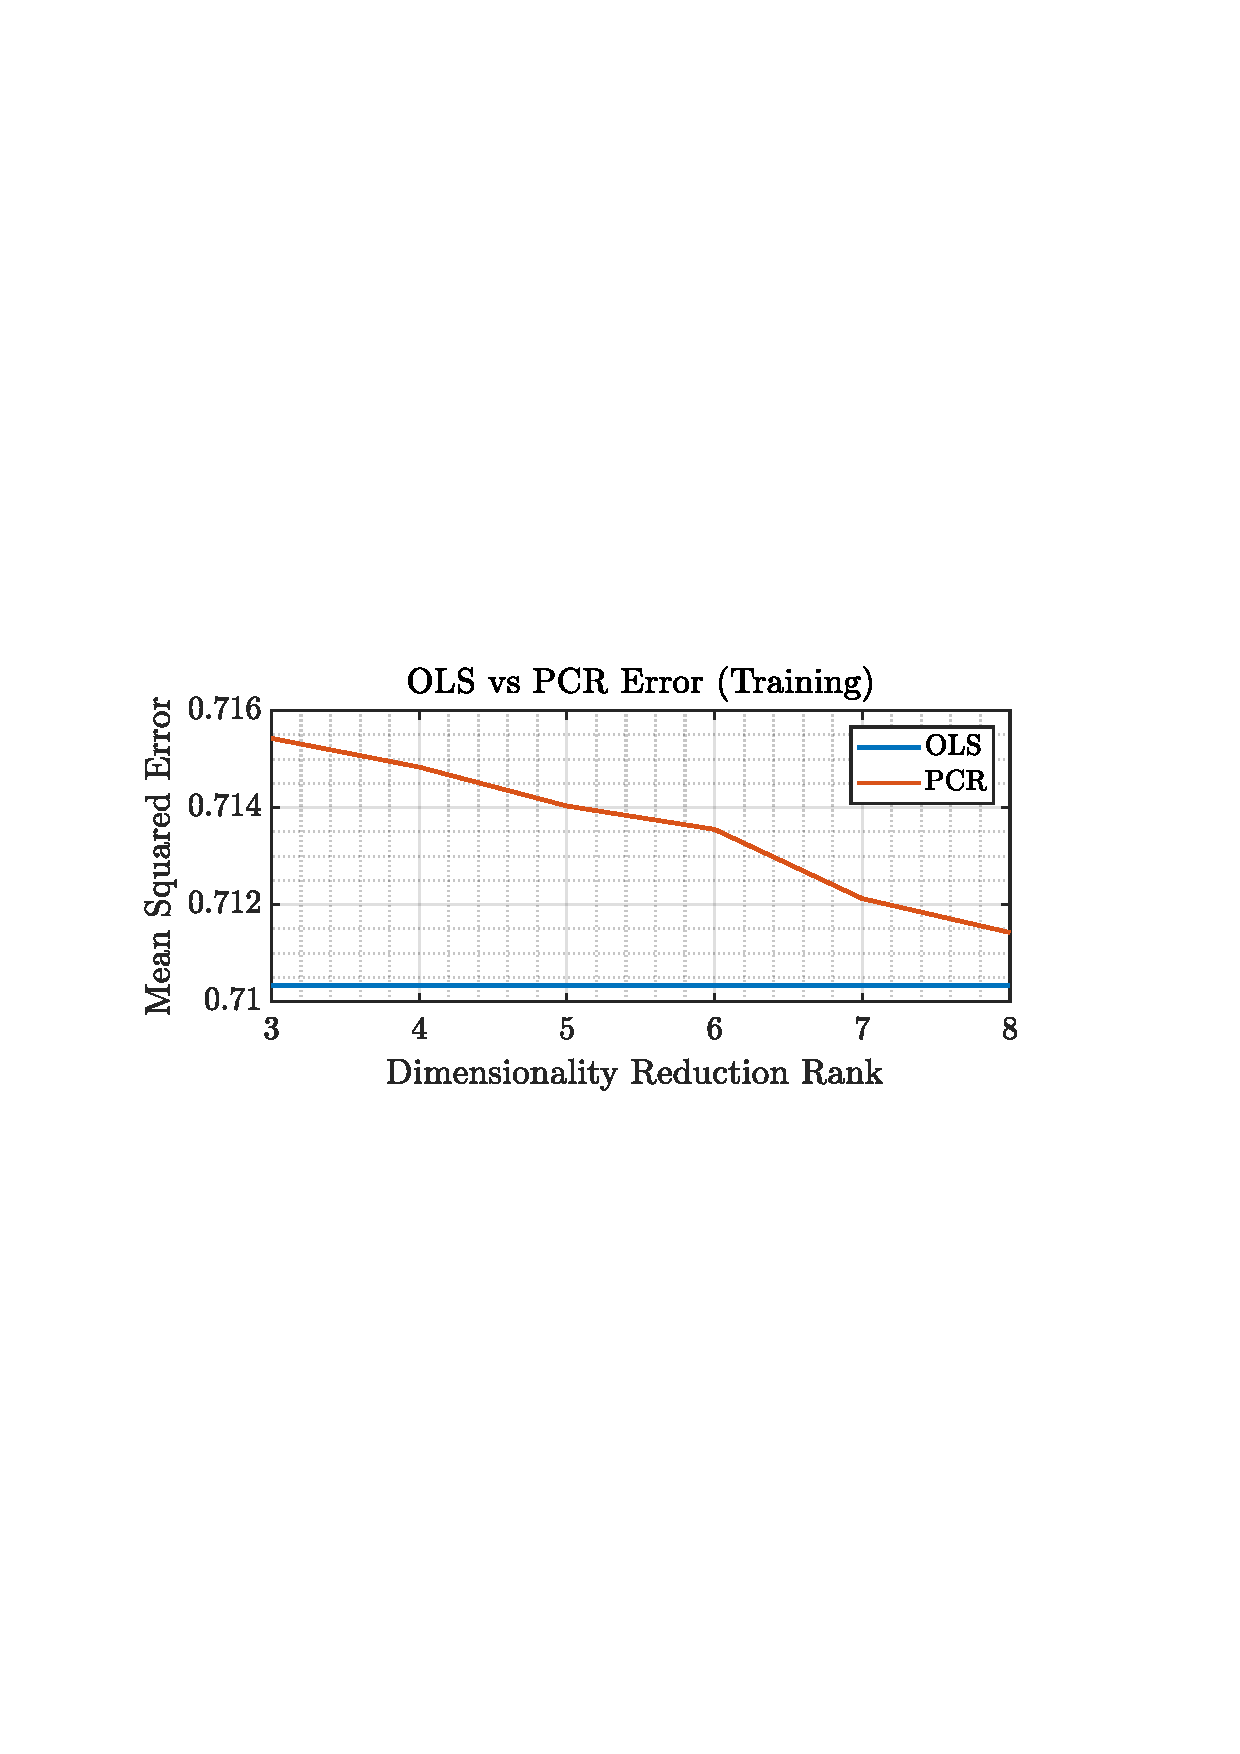
\includegraphics[trim={2.2cm 11.2cm 3.15cm  11.2cm}, clip, width=\textwidth]{../MATLAB/figures/q1_6c_fig01.pdf} 
 			\captionsetup{justification=centering}
 			\caption{Training Dataset Error}
 		\end{subfigure}
 		%		~ % forces onto the same row
 		\begin{subfigure}{0.49\textwidth}
 			\centering
 			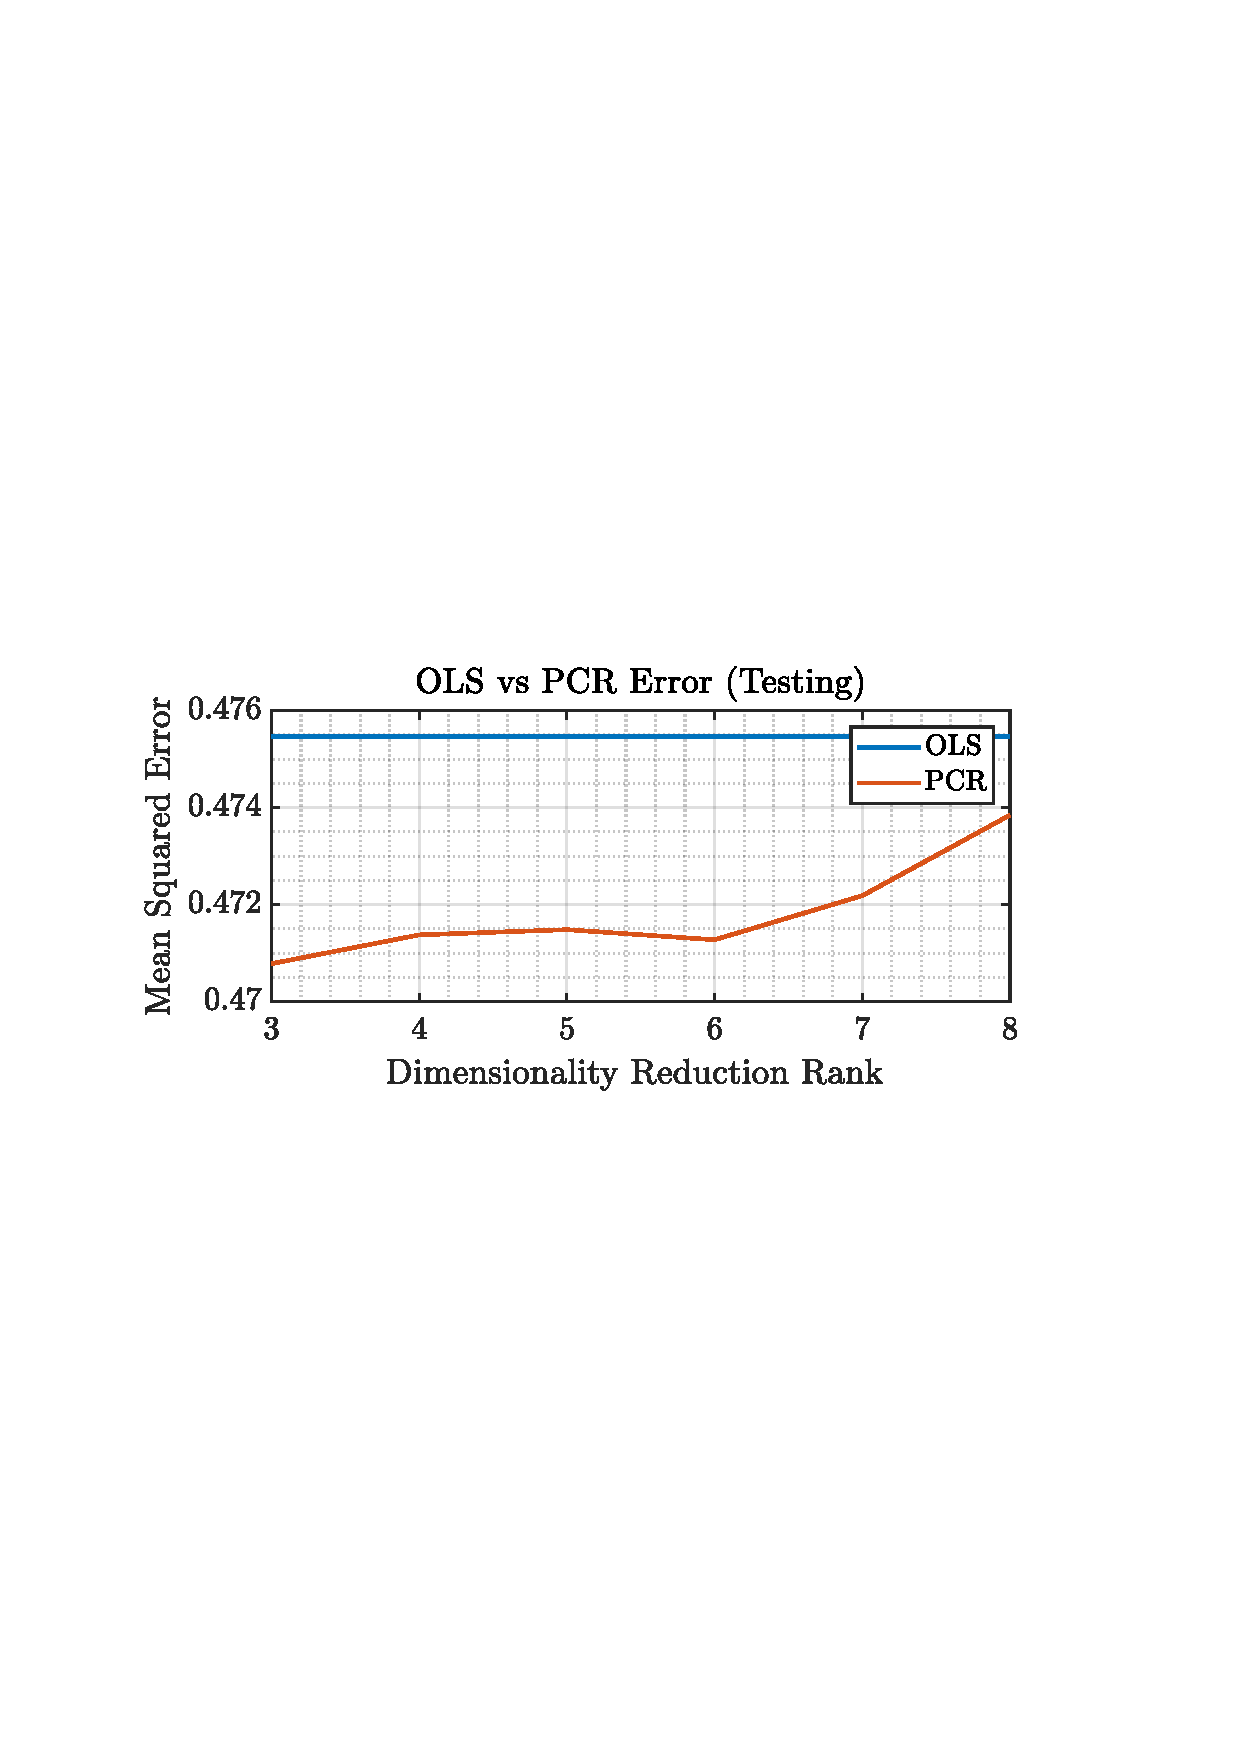
\includegraphics[trim={2.2cm 11.2cm 3.15cm  11.2cm}, clip, width=\textwidth]{../MATLAB/figures/q1_6c_fig02.pdf} 
 			\captionsetup{justification=centering}
 			\caption{Testing Dataset Error}
 		\end{subfigure}
 		\label{fig: 1-6c}
 	\end{figure}


 	\subsubsection{Ordinary Least Squares (OLS) \& Principle Component Regression (PCR)  Estimate Errors - Part 2}
	\begin{figure}[H]
 		\centering
 		\begin{subfigure}{0.49\textwidth}
 			\centering
 			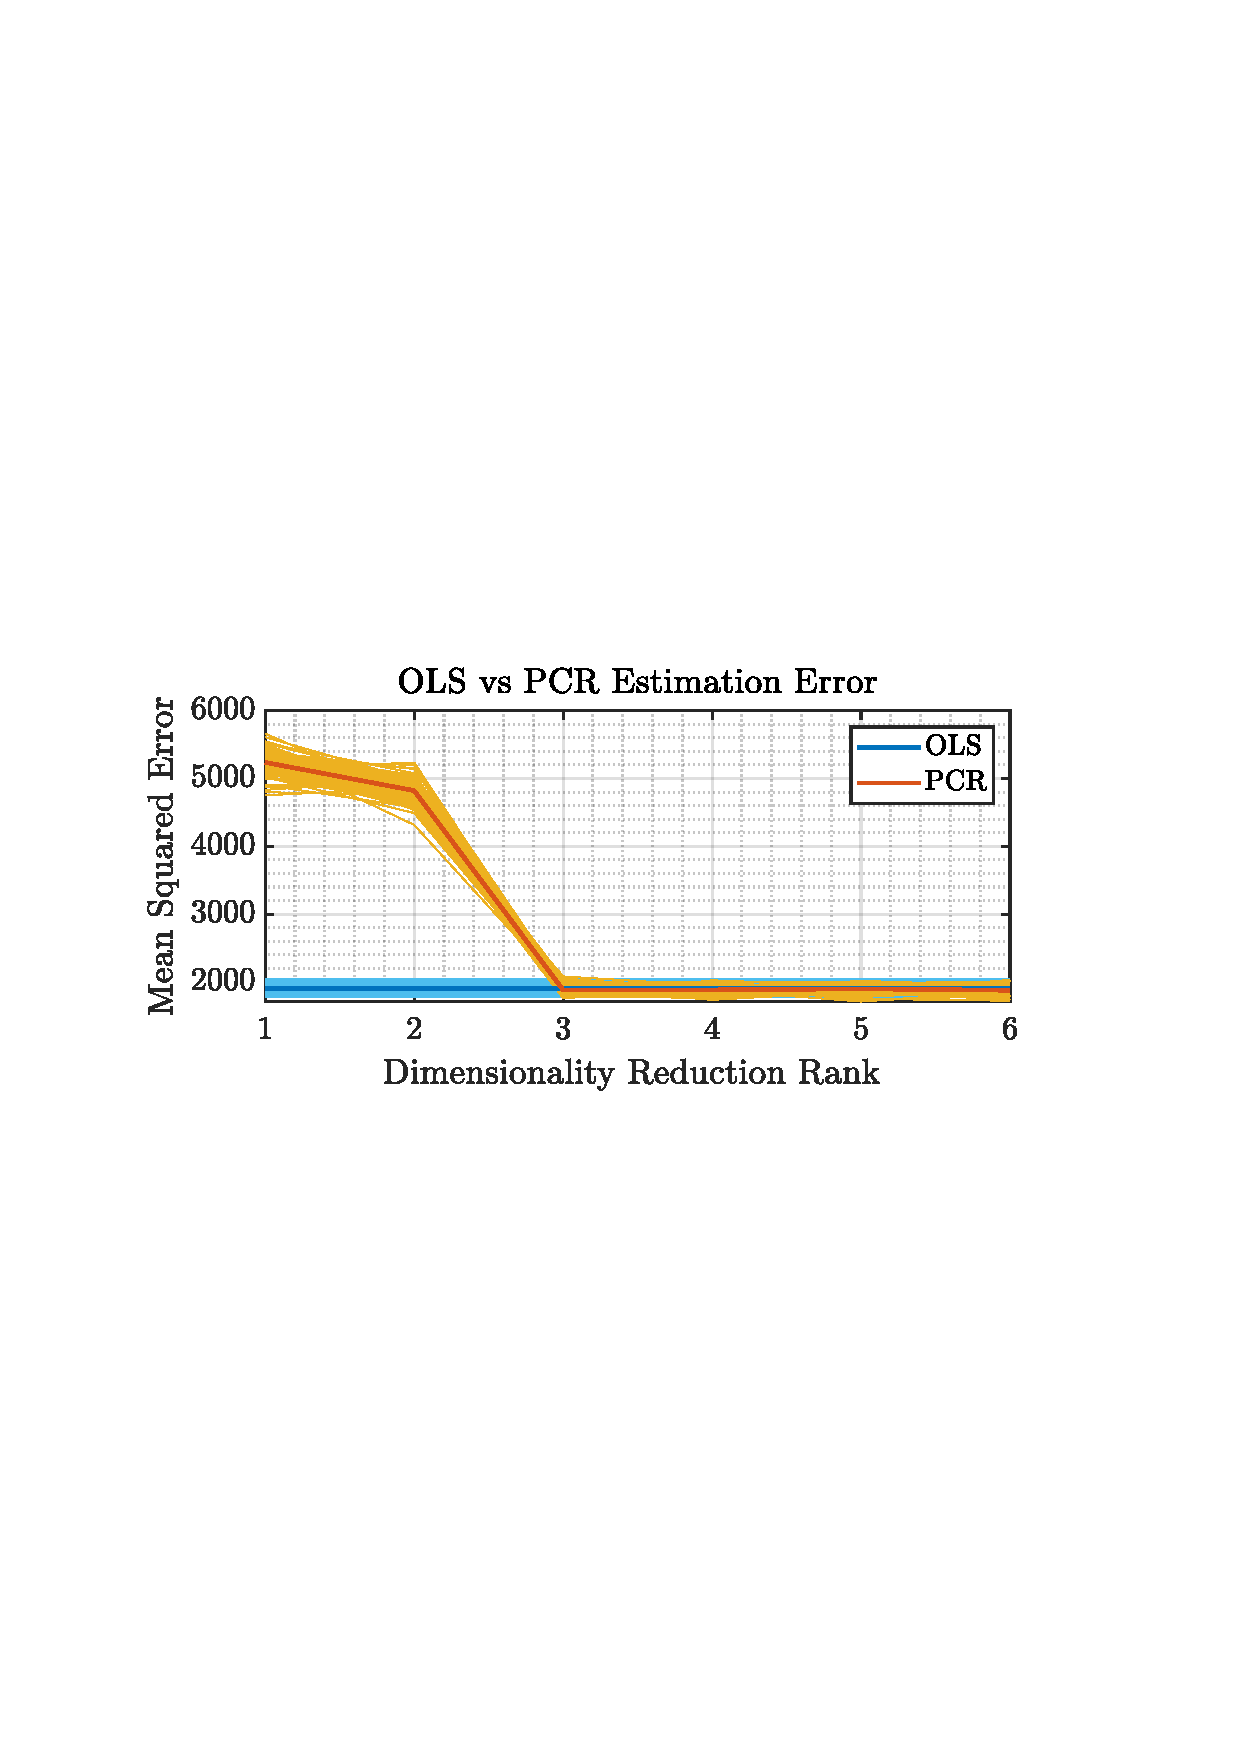
\includegraphics[trim={2.2cm 11.2cm 3.15cm  11.2cm}, clip, width=\textwidth]{../MATLAB/figures/q1_6d_fig01.pdf} 
 			\captionsetup{justification=centering}
 			\caption{Mean Sqaure Error over several Realisations }
 		\end{subfigure}
 		\label{fig: 1-6d}
 	\end{figure}
\end{document}

